\documentclass[12pt,a4paper]{report}
%====En-tête====
% Ajout des packages
\usepackage[english]{babel} % pour dire que le texte est en francais
\usepackage{a4} % pour la taille
\usepackage[T1]{fontenc} % pour les font postscript
\usepackage[cyr]{aeguill} % Police vectorielle TrueType, guillemets francais
\usepackage{epsfig} % pour gérer les images
\usepackage{amsmath,amsthm, mathtools} % très bon mode mathématique
\usepackage{amsfonts,amssymb,bm, bbold}% permet la definition des ensembles
\usepackage{algorithm2e} % pour les algorithmes
\usepackage{algpseudocode} % pour les algorithmes
\usepackage{float} % pour le placement des figure
\usepackage{url} % pour une gestion efficace des url
\usepackage[citecolor=blueind,urlcolor=blue,bookmarks=false,hypertexnames=true]{hyperref}  % pour les hyperliens dans le document
\usepackage{tocbibind} % Pour avoir des index pour table des matières, biblio
\usepackage{tikz} % For graph plots
\usepackage{caption} % Figures
\usepackage{subcaption} % And Subfigures
\usepackage{longtable}
\usepackage{rotating} % For allowing to rotate figures
\usepackage{svg} % To allow svg inclusions

%% Bibliography
\usepackage[style=apa,citestyle=authoryear-comp]{biblatex}
\addbibresource{references.bib}

%% For good md to tex conversion
\providecommand{\tightlist}{%
  \setlength{\itemsep}{0pt}\setlength{\parskip}{0pt}}
\usepackage{booktabs}

%% Tikz Related
\usetikzlibrary{calc,shapes,backgrounds,arrows,automata,shadows,positioning}
\usetikzlibrary{arrows,shapes,positioning,shadows,trees,calc,backgrounds,automata,positioning}



\tikzset{
    basic/.style  = {draw, text width=3cm, font=\sffamily, rectangle},
    root/.style   = {basic, rounded corners=2pt, thin, align=center,
            fill=green!30},
    level 2/.style = {basic, rounded corners=6pt, thin,align=center, fill=green!60,
            text width=8em},
    level 3/.style = {basic, thin, align=left, fill=pink!60, text width=3.5cm}
}


% pour tickz multilevel
\definecolor{redorg}{RGB}{215,48,39}
\definecolor{orangeorg}{RGB}{253,174,97}

\definecolor{blueind}{RGB}{69,117,233}
\definecolor{cyanind}{RGB}{116,173,209}
\definecolor{electricblue}{RGB}{125, 249, 255}

\definecolor{greenind}{RGB}{112,130,56}

\definecolor{burntorange}{RGB}{204, 85, 0}
\definecolor{goldenyellow}{RGB}{255, 192, 0}
\definecolor{yellow}{RGB}{255,255,0}

\definecolor{gray}{RGB}{128,128,128}

% Nouvelles commandes
\newcommand{\Tau}{\mathcal{T}}

% titre et auteur
\title{Rapport de stage dans l'UMR MIA Paris-Saclay}
\author{Louis Lacoste}
\IfFileExists{upquote.sty}{\usepackage{upquote}}{}
\begin{document}
\maketitle
\tableofcontents

\section{Remerciements}

Je tiens à remercier en premier lieu Pierre Barbillon pour son encadrement
remarquable, sa disponibilité, ses conseils avisés et sa gentillesse.
Saint-Clair Chabert-Liddell pour son accompagnement, ses remarques,
ses explications et le temps qu'il m'a consacré. Merci à Sophie Donnet, pour les
cours et les idées qu'elle m'a donné

% TODO Compléter les remerciements

\chapter{L'UMR MIA Paris-Saclay}

\section{Présentation}
L'UMR MIA Paris-Saclay est une entité de recherche qui regroupe des
statisticiens et des informaticiens spécialisés dans la modélisation et
l'apprentissage statistique et informatique appliqués à la biologie, l'écologie,
l'environnement, l'agronomie et l'agro-alimentaire. Elle est affiliée à
AgroParisTech, INRAE et l'Université Paris Saclay.

Les membres de cette unité possèdent des compétences variées en matière de
méthodes d'inférence statistique, telles que les modèles complexes, les modèles
à variables latentes, l'inférence bayésienne, l'apprentissage et la sélection de
modèle. Ils sont également experts en algorithmique, notamment en
généralisation, transfert de domaine et représentation des connaissances.

L'objectif de cette unité est de développer des méthodes statistiques et
informatiques originales, à la fois génériques et motivées par des
problématiques spécifiques dans le domaine des sciences du vivant. Les activités
de recherche s'appuient sur une solide culture dans les disciplines cibles,
telles que l'écologie, l'environnement, l'agro-alimentaire, la biologie
moléculaire et la biologie des systèmes.

L'unité est structurée en deux équipes de recherche : SOLsTIS (Statistical
mOdelling and Learning for environnemenT and lIfe Sciences) et EkINocs (Expert
Knowledge, INteractive modellINg and learnINg for understandINg and decisiOn
makINg in dINamic Complexe Systems).

Elle est rattachée au département MATHNUM d'INRAE et au département MMIP
d'AgroParisTech.

Les responsables au sein de l'unité sont : Julien Chiquet en tant que Directeur
d'unité, Sophie Donnet en tant que Directrice d'unité adjointe, Antoine
Cornuéjols en tant que Responsable de l'équipe EkINocs, et Sophie Donnet
et Pierre Barbillon en tant que Responsables de l'équipe SOLsTIS.
\newline
\emph{Source:~\cite{AccueilMIAParisSaclay}}\\
La figure \ref{fig:organigramme-umr} présente l'organigramme complet de l'unité.

\begin{sidewaysfigure}[h!]
    \begin{center}
        % 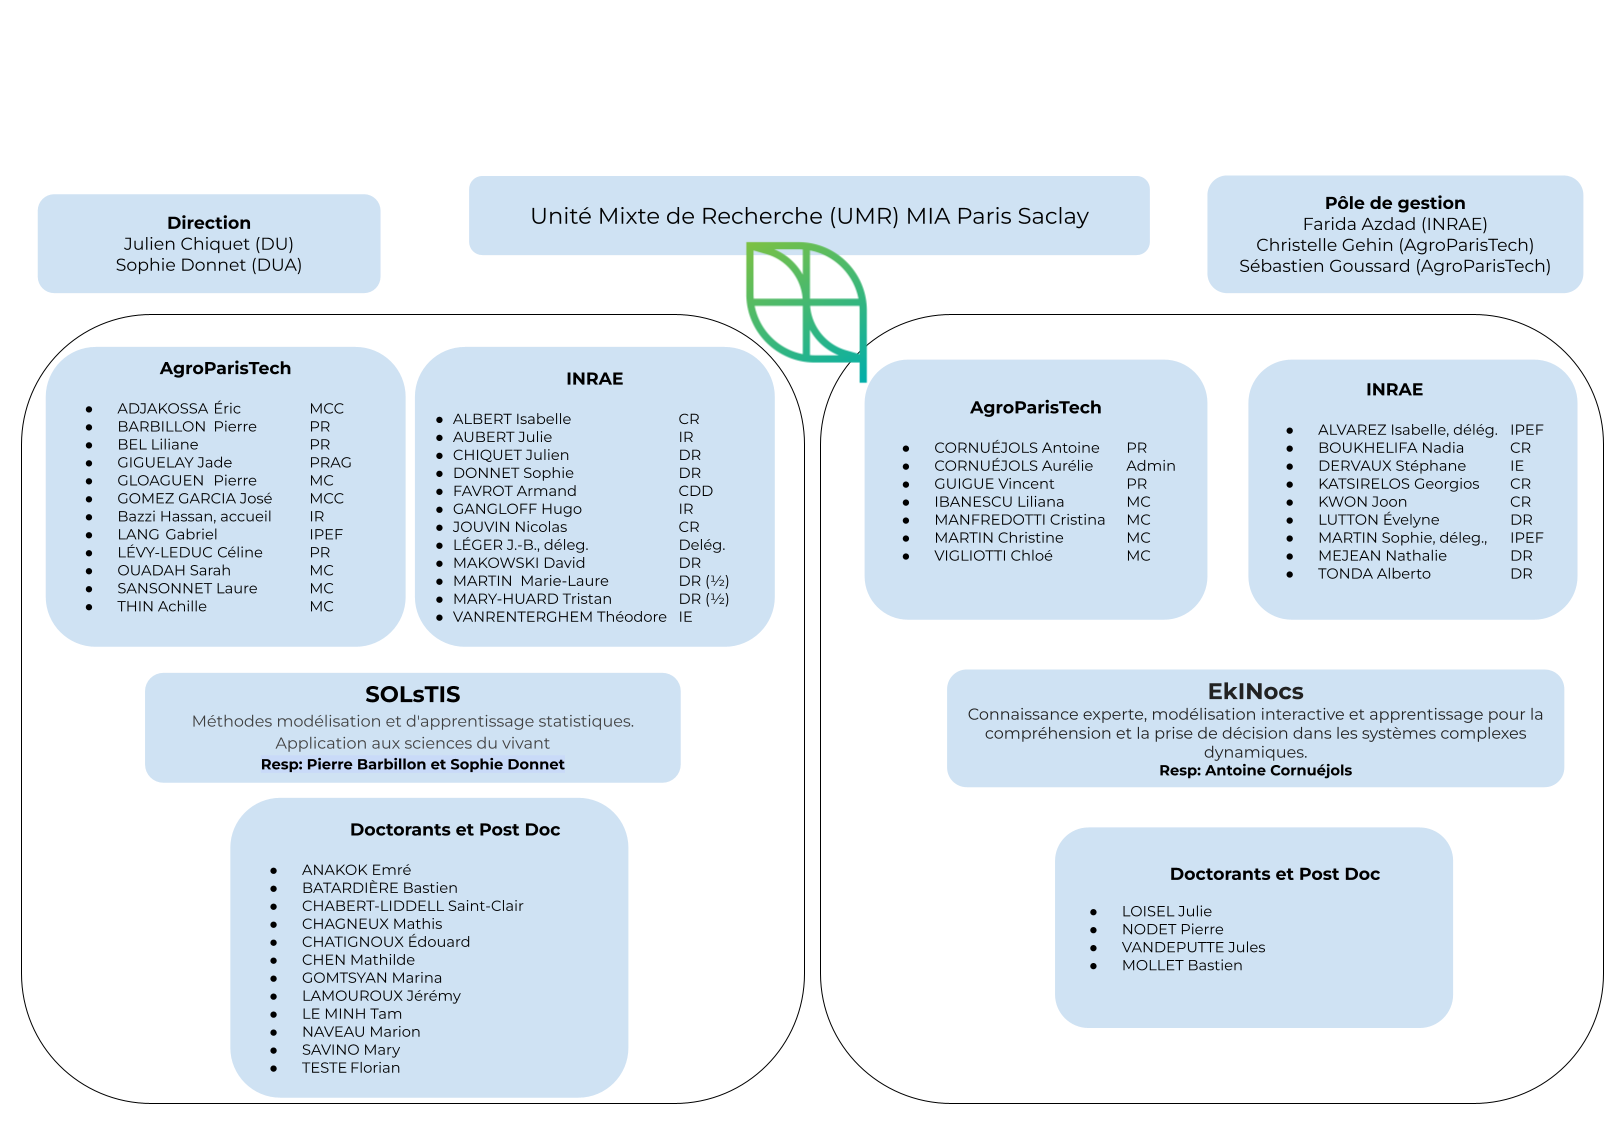
\includegraphics[scale=0.4]{img/Organigramme_MIA-Paris-Saclay}
        \includesvg[scale=0.6]{img/Organigramme_MIA-Paris-Saclay.svg}
        \caption{Organigramme de l'UMR}
        \label{fig:organigramme-umr}
    \end{center}
\end{sidewaysfigure}

\section{Encadrement et vie en stage}

Au cours de mon stage, j'étais encadré par Pierre Barbillon et fréquemment en
discussion avec lui et Saint-Clair Chabert-Liddell dont j'ai poursuivi les
travaux.

Le contexte de travail, au sein des ingénieurs d'études, des doctorants, des
chercheurs et des maîtres de conférences, a été pour moi très enrichissant. Ce
stage s'inscrit dans la construction de mon parcours professionnel en validant
le désir que je présentais de faire de la recherche.

Par ailleurs, divers projets entrepris au sein du laboratoire ont permis de
nouer des relations amicales en dehors des heures de travail. Par exemple, le
projet de construction d'une borne d'arcade pour le laboratoire, impulsé par
Julien Chiquet, a été une expérience extrêmement agréable et captivante à
laquelle prendre part.

J'ai particulièrement apprécié la disponibilité de toutes les personnes de
l'unité qui n'ont jamais hésité à se rendre disponible pour répondre à mes
questions.
Les nombreux séminaires et le désir de partage de connaissances à travers des
formations internes et de l'auto-formation m'a vraiment plu et m'a ouvert à de
nouvelles problématiques passionnantes.
De plus j'ai beaucoup progressé dans les domaines abordés pendant mon
stage, et cela m'a rendu confiant dans le choix de faire le
master \emph{MathSV} pour l'année scolaire 2023-2024. Ce stage a donc été
déterminant et confirme l'orientation de mon parcours professionnel.

\paragraph*{Note} La suite de ce rapport a été rédigée en anglais.

\chapter{Context of the study}

\section{Usage and importance of bipartite graphs}
\label{sec:usage-and-importance-of-bipartite-graphs}
Bipartite graphs, denoted as $G = (U,V,E)$ with $U$ and $V$ two disjoint and
independent sets of vertices and $E$ the set of edges connecting $U$ vertices to
$V$ vertices.

\begin{minipage}{0.5\linewidth}
    \centering
    Bipartite network\\
    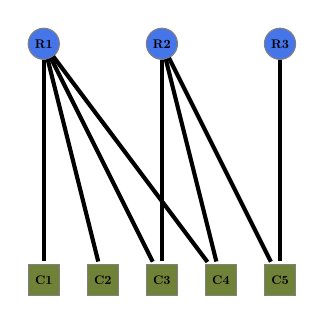
\begin{tikzpicture}[scale=.6]
        \tikzstyle{every edge}=[-,>=stealth',shorten >=1pt,auto,draw,line width=1.5pt]
        \tikzstyle{every state}=[draw, text=black,scale=0.95, transform shape]
        \tikzstyle{every state}=[draw=none,text=black,scale=0.75, transform shape]
        \tikzstyle{every node}=[fill=blueind]

        \node[state, draw=black!50] (A1) at (0,5) {\textbf{R1}};
        \node[state, draw=black!50] (A2) at (2.5,5) {\textbf{R2}};
        \node[state, draw=black!50] (A3) at (5,5) {\textbf{R3}};

        \tikzstyle{every node}=[fill=greenind, shape=rectangle]
        \tikzstyle{every state}=[draw=none,text=black,scale=0.75, transform shape, shape=rectangle]
        \node[state, draw=black!50] (B1) at (0,0) {\textbf{C1}};
        \node[state, draw=black!50] (B2) at (1.25,0) {\textbf{C2}};
        \node[state, draw=black!50] (B3) at (2.5,0) {\textbf{C3}};
        \node[state, draw=black!50] (B4) at (3.75,0) {\textbf{C4}};
        \node[state, draw=black!50] (B5) at (5,0) {\textbf{C5}};
        \path (A1) edge [] (B1);
        \path (A1) edge  (B2);
        \path (A1) edge  (B3);
        \path (A1) edge  (B4);
        \path (A2) edge  (B3);
        \path (A2) edge  (B4);
        \path (A3) edge  (B5);
        \path (A2) edge  (B5);
    \end{tikzpicture}
\end{minipage}
\begin{minipage}{0.5\linewidth}
    \begin{center}
        Incidence matrix
        $X=\left(
            \begin{array}{rrrrr}
                1 & 1 & 1 & 1 & 0 \\
                0 & 0 & 1 & 1 & 1 \\
                0 & 0 & 0 & 0 & 1 \\
            \end{array}\right)
        $\\
    \end{center}
\end{minipage}

$X$ is the \emph{incidence matrix} and is the mathematical object on which
computations are performed. It is filled with the following rule:
\begin{equation*}
    \begin{cases}
        X_{ij} = 0 & \text{if no interaction is observed between species }i\text{ and }j\\
        X_{ij} \neq 0 & \text{otherwise}
    \end{cases}
\end{equation*}
If the network represents binary observation (like presence-absence observation) then
$X_{ij}\in\mathcal{K}=\{0,1\},\forall(i,j)$; if the interactions are weighted
(like an abundance count), $X_{ij}\in\mathcal{K}=\mathbb{N},\forall(i,j)$.

This representation can be used to represent various forms of interactions were
two kinds of ``actors`` interact. Those interactions can be binary or valued and
a numeric representation is the incidence matrix, in the above example $X$.\\

Among the use case of bipartite graphs one can find the Netflix Problem, which
was a prize organized by Netflix to improve its Recommender system. The row
nodes are the movies and the columns are the user, at the intersection the value
is the review of the user $j$ for the movie $i$.\\

Another use is the representation of ecological interactions like
plant-pollinator \parencite{ramos-jilibertoTopologicalChangeAndean2010}, birds-seed
dispersion, prey-predator or
host-parasite \parencite{kaszewska-gilasGlobalStudiesHostParasite2021}.
In those cases, the rows are pollinator species and the columns are plant
species, and the intersection is a value, binary if it is a presence/absence or
a value if it is an abundance count.

Bipartite graphs are widely used in biology, in various fields, among which the
previously cited ecological networks, but also in medicine with biomedical
networks, biomolecular networks or epidemiological
networks. \parencite{pavlopoulosBipartiteGraphsSystems2018}


Some interesting results can arise when applying a tool widely used on a particular
kind of interactions is used on another kind of interactions. Companies like
Netflix use recommender system, to recommend another product to consumers based
on their previous interactions.
In ~\cite{desjardins-proulxEcologicalInteractionsNetflix2017} the authors use the
\emph{K-nearest neighbour} (KNN) algorithm as a Recommender to predict missing
preys for predators in a predator-prey network.

\section{Latent Block Model}
\label{sec:latent-block-model}
The Latent Block Model (LBM) introduced by ~\cite{govaertLatentBlockModel2010}
adapts the Stochastic Block Model (SBM)
(~\cite{hollandStochasticBlockmodelsFirst1983};~\cite{snijdersEstimationPredictionStochastic1997})
to bipartite graphs.

\begin{small}
    Please note that we prefer the term ``BiSBM`` and will use both LBM and BiSBM to
    designate the Stochastic Block model applied on bipartite networks.
\end{small}

This model supposes that:
\begin{itemize}
    \item Row nodes are members of row blocks and column nodes are members of
          column blocks.
    \item The connectivity of two individuals is determined by their block
          memberships.
    \item An interaction can only occur between a row and a column node.
\end{itemize}

\begin{figure}[H]
    \center
    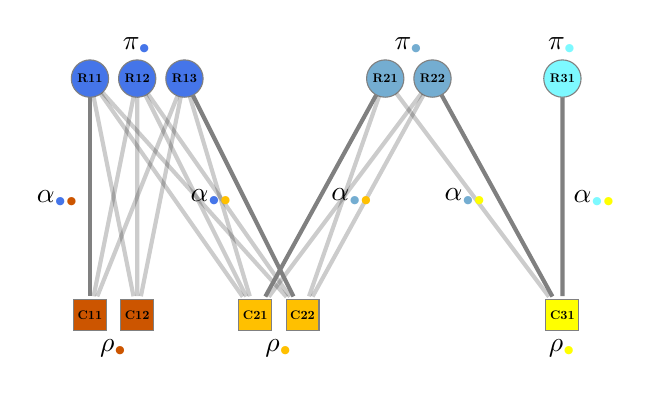
\begin{tikzpicture}[scale=.6]
        \tikzstyle{every state}=[draw, text=black,scale=0.95, transform shape]
        \tikzstyle{every state}=[draw=none,text=black,scale=0.75, transform shape]
        \tikzset{edge_proba/.style={draw=white, fill=none, text=black}}

        \tikzstyle{every node}=[fill=blueind]
        \node[edge_proba] (pi1) at (1,5.7) {\textbf{$\pi_{{\color{blueind}\bullet}}$}};
        \node[state, draw=black!50] (R11) at (0,5) {\textbf{R11}};
        \node[state, draw=black!50] (R12) at (1,5) {\textbf{R12}};
        \node[state, draw=black!50] (R13) at (2,5) {\textbf{R13}};

        \tikzstyle{every node}=[fill=cyanind]
        \node[edge_proba] (pi2) at (6.75,5.7) {\textbf{$\pi_{{\color{cyanind}\bullet}}$}};
        \node[state, draw=black!50] (R21) at (6.25,5) {\textbf{R21}};
        \node[state, draw=black!50] (R22) at (7.25,5) {\textbf{R22}};

        \tikzstyle{every node}=[fill=electricblue]
        \node[edge_proba] (pi3) at (10,5.7) {\textbf{$\pi_{{\color{electricblue}\bullet}}$}};
        \node[state, draw=black!50] (R31) at (10,5) {\textbf{R31}};

        \tikzstyle{every node}=[fill=burntorange, shape=rectangle]
        \node[edge_proba] (pi3) at (0.5,-0.7) {\textbf{$\rho_{{\color{burntorange}\bullet}}$}};
        \tikzstyle{every state}=[draw=none,text=black,scale=0.75, transform shape, shape=rectangle]
        \node[state, draw=black!50] (B1) at (0,0) {\textbf{C11}};
        \node[state, draw=black!50] (B2) at (1,0) {\textbf{C12}};
        \tikzstyle{every node}=[fill=goldenyellow, shape=rectangle]
        \node[edge_proba] (pi3) at (4,-0.7) {\textbf{$\rho_{{\color{goldenyellow}\bullet}}$}};
        \node[state, draw=black!50] (B3) at (3.5,0) {\textbf{C21}};
        \node[state, draw=black!50] (B4) at (4.5,0) {\textbf{C22}};
        \tikzstyle{every node}=[fill=yellow, shape=rectangle]
        \node[edge_proba] (pi3) at (10,-0.7) {\textbf{$\rho_{{\color{yellow}\bullet}}$}};
        \node[state, draw=black!50] (B5) at (10,0) {\textbf{C31}};

        \tikzstyle{every edge}=[-,>=stealth',shorten >=1pt,auto,draw,line width=1.5pt,draw opacity=0.2]

        \path (R11) edge (B2);
        \path (R11) edge  (B3);
        \path (R11) edge  (B4);

        \path (R12) edge [] (B1);
        \path (R12) edge  (B2);
        \path (R12) edge  (B3);
        \path (R12) edge  (B4);

        \path (R13) edge [] (B1);
        \path (R13) edge  (B2);
        \path (R13) edge  (B3);


        \path (R21) edge  (B4);
        \path (R21) edge  (B5);

        \path (R22) edge  (B3);
        \path (R22) edge  (B4);

        \path (R11) edge[-,>=stealth',shorten >=1pt,auto,draw=gray,line width=1.5pt, fill=gray, opacity=1] node[left, fill=none] {$\alpha_{{\color{blueind}\bullet}{\color{burntorange}\bullet}}$} (B1);
        \path (R13) edge[-,>=stealth',shorten >=1pt,auto,draw=gray,line width=1.5pt, fill=gray, opacity=1] node[midway, left, fill=none] {$\alpha_{{\color{blueind}\bullet}{\color{goldenyellow}\bullet}}$} (B4);
        \path (R21) edge[-,>=stealth',shorten >=1pt,auto,draw=gray,line width=1.5pt, fill=gray, opacity=1] node[midway, right, fill=none] {$\alpha_{{\color{cyanind}\bullet}{\color{goldenyellow}\bullet}}$} (B3);
        \path (R22) edge[-,>=stealth',shorten >=1pt,auto,draw=gray,line width=1.5pt, fill=gray, opacity=1] node[midway, left, fill=none] {$\alpha_{{\color{cyanind}\bullet}{\color{yellow}\bullet}}$} (B5);
        \path (R31) edge[-,>=stealth',shorten >=1pt,auto,draw=gray,line width=1.5pt, fill=gray, opacity=1] node[midway, right, fill=none] {$\alpha_{{\color{electricblue}\bullet}{\color{yellow}\bullet}}$} (B5);

    \end{tikzpicture}
    \caption{An LBM model visualization}
    \label{fig:LBMvisu}
\end{figure}

Parameters
% TODO fix parameters according to presentation
\begin{itemize}
    \item $Q_1 = \{{\color{blueind}\bullet},{\color{cyanind}\bullet},{\color{electricblue}\bullet}\}$ blocks in rows
    \item $Q_2 = \{{\color{burntorange}\bullet},{\color{goldenyellow}\bullet},{\color{yellow}\bullet}\}$ blocks in columns
    \item $\pi_{\bullet} = \mathbb{P}(i\in\bullet)$ in row and $\rho_{\bullet} = \mathbb{P}(j\in\bullet)$ in column
    \item $\alpha_{{\color{blueind}\bullet}{\color{burntorange}\bullet}} = \mathbb{P}(i \leftrightarrow j | i \in {\color{blueind}\bullet}, j \in {\color{burntorange}\bullet})$ connectivity probability between two nodes, given their clustering
\end{itemize}

On \ref{fig:LBMvisu}, $\pi$ are the probabilities for a row node to belong to
the row block of corresponding color, $\rho$ are the probabilities for a column
node to belong to the column block of corresponding color and $\alpha$ are the
connectivity parameters between the row and column blocks.

This model can be used to easily generate bipartite graphs with complex and very
varied structures. But when trying to determine the structure of a given network
we need to find those parameters.

For this a common approach is to use a VEM algorithm
(proposed for SBM in ~\cite{daudinMixtureModelRandom2008} and for LBM in ~\cite{govaertEMAlgorithmBlock2005})
those groups and the required parameters can be inferred by maximizing a lower
bound of the likelihood minus a penalty.

\section{colSBM model, a joint model for a collection of networks}
\label{sec:colsbm-model-a-joint-model-for-a-collection-of-networks}
The \emph{colSBM} model introduced by ~\cite{chabert-liddellLearningCommonStructures2023}
propose an extension of the SBM model to collections of SBMs. A collection is a
set of networks which nodes are not common or linked between different networks,
the interactions have the same valuations and are of the same type.

The model can retrieve the shared structure in a collection, indicate
if networks should be grouped in a collection and  in a large pool of networks,
collections with common structures.

The next step after designing this collection model for unipartite was to adapt
it to the bipartite case.

\chapter{Structure detection in a collection of bipartite networks : Adjustment of colSBM to the bipartite case}
\section{Definition of a collection}\label{sec:definition-of-a-collection}

We define a collection of bipartite networks as $\bm{X} = (X^1, \dots, X^M)$
the collection of incidence matrix. Moreover, all the networks in the collection
have the same type of interaction (e.g., all interactions are binary).

\section{Separate BiSBM (sepBiSBM)}\label{sec:separate-bisbm-sepbisbm}

A first approach to deal with a collection of networks is to adjust separate
BiSBM for each network of the collection.

For network $m$, let $n_1^m$ (resp. $n_2^m$) be the number of nodes in row
(resp. column) divided into $Q_1^m$ row clusters (resp. $Q_2^m$ column
clusters).\\
Let $Z^m~=~(Z^m_i, \dots, Z^m_{n_1^m})$ and $W^m~=~(W^m_j, \dots, W^m_{n_2^m})$
be independent latent variables such that $Z^m_i = q$ if row node $i$ of network
$m$ belongs to row cluster $q$ ($q\in\{1,\dots,Q_1^m\}$) and $W^m_j = r$ if column node $j$ of network $m$
belong to column block $r$ ($r\in\{1,\dots,Q_2^m\}$). And we have
\begin{align}\label{eqn:lbm-block-membership-prob}
    \mathbb{P}(Z_i^m=q)=\pi_q^m,&&\mathbb{P}(W_j^m=r)=\rho_r^m
\end{align}
where $\pi_q^m > 0$, $\rho_r^m > 0$, $\sum_{q=1}^{Q_1^m}\pi_q^m = 1$ and
$\sum_{r=1}^{Q_2^m}\rho_r^m = 1$. Given the latent variables
$Z^m, W^m$, the $X_{ij}^m$s are assumed to be independent and distributed
as

\begin{align}\label{eqn:lbm-conditional-to-latent}
    X_{ij}^m|Z_i^m = q,W_j^m = r \sim \mathcal{F}(.;\alpha_{qr}^m)
\end{align}
where $\mathcal{F}$ is referred to as the emission distribution. $\mathcal{F}$ is chosen to
be the Bernoulli distribution for binary interactions, and the Poisson
distribution for weighted interactions such as counts. Let $f$ be the density of
the emission distribution, then:

\begin{equation}\label{eqn:lbm-emission}
    \log f(X^m_{ij};\alpha_{qr}^m) =
    \begin{cases}
        X_{ij}^m \log(\alpha_{qr}^m) + (1-X_{ij}^m) \log(1-\alpha_{qr}^m) & \text{for Bernoulli emission} \\
        -\alpha_{qr}^m + X_{ij}^m \log(\alpha_{qr}^m) - \log(X_{ij}^m!) & \text{for Poisson emission}
    \end{cases}
\end{equation}

Equations \eqref{eqn:lbm-block-membership-prob}, \eqref{eqn:lbm-conditional-to-latent}
and \eqref{eqn:lbm-emission} defines the BiSBM model and we will now use a short
notation:

\begin{equation}
    \tag{\emph{sep-BiSBM}}
    X^m \sim \mathcal{F}\text{-BiSBM}_{n_1^m,n_2^m}(Q_1^m, Q_2^m, \bm{\pi^m}, \bm{\rho^m}, \bm{\alpha^m})
\end{equation}
where $\mathcal{F}$ encodes the emission distribution, $n_1^m,n_2^m$ are the row
and column nodes, $Q_1^m, Q_2^m$ are the number of row and column blocks in
network $m$, $\bm{\pi}^m~=~{(\pi^m_q)}_{q=1,\dots,Q_1^m}$ and
$\bm{\rho}^m~=~{(\rho^m_r)}_{r=1,\dots,Q_2^m}$ are the vectors  of their
proportions. The $Q_1^m \times Q_2^m$ matrix
$\bm{\alpha}^m = {(\alpha^m_{qr})}_{\substack{q = 1,\dots,Q_1^m \\ r = 1,\dots,Q_2^m}}$
are the connectivity parameters, the parameters of the emission distribution.
$\alpha^m_{qr}\in\mathcal{A}_{\mathcal{F}}$ where, for the Bernoulli
(resp. Poisson) emission distribution, $\mathcal{A}_{\mathcal{F}} = (0,1)$ (resp.
$\mathcal{A}_{\mathcal{F}} = \mathbb{R}^{*+}$). In this $sep$-$BiSBM$ each
network $m$ is assumed to follow a $BiSBM$ with its own parameters ($\bm{\pi}^m,
\bm{\rho}^m, \bm{\alpha}^m$).
% DONE Finish explaining

\section{Definition of the colBiSBM models}\label{sec:definition-of-the-colbisbm-models}
% Here are some common notations and conventions that we will use in the following
% sections.

\subsection{A collection of i.i.d bipartite SBM}\label{ssec:a-collection-of-i-i-d-bipartite-sbm}
As for \emph{colSBM} this first model is the most constrained. It assumes
that all the networks are the independent realizations of the same $Q_1$-$Q_2$-BiSBM
with identical parameters. The \emph{iid-colBiSBM} is defined as follows:

\begin{align}
    \tag{\emph{iid-colBiSBM}}
    X^m \sim \mathcal{F}-BiSBM_{n_1^m,n_2^m} (Q_1, Q_2, \bm{\pi}, \bm{\rho}, \bm{\alpha}), && \forall m = 1, \dots M
\end{align}
where $\forall (q,r) \in \{1,\dots,Q_1\}\times\{1,\dots,Q_2\}$, $\alpha_{qr} \in \mathcal{A}_{\mathcal{F}}$,
$\pi_q \in \left( 0,1 \right], \sum_{q=1}^{Q_1} \pi_q = 1 $ and $\rho_r \in \left( 0,1 \right], \sum_{r=1}^{Q_2} \rho_r = 1 $.
This model involves $(Q_1 - 1) + (Q_2 - 1) + Q_1\times Q_2$ parameters, the two
first terms corresponding to block proportions on the row and column dimensions
and the third term to connectivity parameters.

But the assumption that block proportions are the same among the networks is a
strong assumption. In plant-pollinator networks, the proportion of specialist
species can differ between networks and thus the model may benefit from not
having the same block proportions but sharing a common connectivity structure.
The following models relaxes this assumption on either row, column or both.

\subsection{A collection of bipartite SBM with varying block size on either rows or columns}\label{ssec:a-collection-of-bipartite-sbm-with-varying-block-size-on-either-rows-or-columns}
% DONE Finish explaining

$\pi$-colBiSBM model still assumes that the networks share a common connectivity
structure represented by $\bm{\alpha}$ but that each network has its own row
block proportions. For $m \in \{1,\dots,M\}$, the $X^m$ are independent and
\begin{align}
    \tag{\emph{$\pi$-colBiSBM}}
    X^m \sim \mathcal{F}-BiSBM_{n_1^m,n_2^m} (Q_1, Q_2, \bm{\pi^m}, \bm{\rho}, \bm{\alpha}), && \forall m = 1, \dots, M
\end{align}
where $\forall (q,r) \in \{1,\dots,Q_1\}\times\{1,\dots,Q_2\}$, $\alpha_{qr} \in \mathcal{A}_{\mathcal{F}}$,
$\pi^m_q \in \left[ 0,1 \right], \sum_{q=1}^{Q_1} \pi^m_q~=~1, \forall m \in \{1,\dots,M\}$ and $\rho_r \in \left( 0,1 \right], \sum_{r=1}^{Q_2} \rho_r = 1 $.
This model is more flexible than the iid-colBiSBM as it allows some row block
proportions to be null
in certain networks ($\pi^m_q\in\left[ 0,1 \right]$): if $\pi_q^m = 0$ then the
block $q$ is not represented in the network $m$. The connectivity structure is
thus a subset of a large connectivity structure common to all networks. We face
the same problems as~\cite{chabert-liddellLearningCommonStructures2023} and
adapt the support $S$ they define for the $\pi$-colSBM to the bipartite case by
having $S^1$ of size $M\times Q_1$ the support for the rows and $S^2$ of size
$M\times Q_2$ the support for the columns. Thus
$S^1_{mq} = \mathbb{1}_{\pi^m_q > 0}$ and
$S^2_{mr} = \mathbb{1}_{\rho^m_r > 0}$. In this case, $S^2 = \bm{1}$, because
there is no freedom on the column dimension.

For a given number of blocks $Q_1$, $Q_2$ and matrix $S^1$ ($S^2$ being in this case the matrix full of ones), the number of
parameters is:
\begin{equation*}
    \text{NP}(\pi\text{-}colBiSBM) = \sum_{m=1}^{M}\Bigg( \sum_{q=1}^{Q_1} S^1_{mq} - 1 \Bigg) + (Q_2 - 1) + \sum_{\substack{q=1,\dots,Q_1 \\ r=1,\dots,Q_2}} \mathbb{1}_{{(S^{1\prime}S^2)}_{qr}>0}
\end{equation*}
The first term corresponds to the non-null block proportions in each network.
The third quantity accounts for the fact that some blocks may never be
represented simultaneously in any network, so the corresponding connection
parameters $\alpha_{qr}$ are not useful for defining the model.

$\rho$-colBiSBM model still assumes that the networks share a common connectivity
structure represented by $\bm{\alpha}$ but that each network has its own column
block proportions. For $m \in \{1,\dots,M\}$, the $X^m$ are independent and
\begin{align}
    \tag{\emph{$\rho$-colBiSBM}}
    X^m \sim \mathcal{F}-BiSBM_{n_1^m,n_2^m} (Q_1, Q_2, \bm{\pi}, \bm{\rho^m}, \bm{\alpha}), && \forall m = 1, \dots, M
\end{align}
where $\forall (q,r) \in \{1,\dots,Q_1\}\times\{1,\dots,Q_2\}$, $\alpha_{qr} \in \mathcal{A}_{\mathcal{F}}$,
$\pi_q \in \left( 0,1 \right], \sum_{q=1}^{Q_1} \pi_q = 1 $ and
$\rho^m_r \in \left[ 0,1 \right], \sum_{r=1}^{Q_2} \rho^m_r = 1 $.
This model is more flexible than the iid-colBiSBM as it allows some column block
proportions to be
null in certain networks ($\rho^m_r\in\left[ 0,1 \right]$): if $\rho_r^m = 0$
then the column block $r$ is not represented in the network $m$.
"Mirroring" the formulas for the $\pi$-$colBiSBM$ we relax the constraints on
the column dimension.

For a given number of blocks $Q_1$, $Q_2$ and matrix $S^2$ ($S^1$ being in this case the matrix full of ones), the number of
parameters is:
\begin{equation*}
    \text{NP}(\rho\text{-}colBiSBM) = (Q_1 - 1) + \sum_{m=1}^{M}\Bigg( \sum_{r=1}^{Q_2} S^2_{mr} - 1 \Bigg) + \sum_{\substack{q=1,\dots,Q_1 \\ r=1,\dots,Q_2}} \mathbb{1}_{{(S^{1\prime}S^2)}_{qr}>0}
\end{equation*}

$\pi\rho$-colBiSBM model still assumes that the networks share a common connectivity
structure represented by $\bm{\alpha}$ but that each network has its own row and
column block proportions, it is the less constrained model.
For $m \in \{1,\dots,M\}$, the $X^m$ are independent and
\begin{align}
    \tag{\emph{$\pi\rho$-colBiSBM}}
    X^m \sim \mathcal{F}-BiSBM_{n_1^m,n_2^m} (Q_1, Q_2, \bm{\pi^m}, \bm{\rho^m}, \bm{\alpha}), && \forall m = 1, \dots, M
\end{align}
where $\forall (q,r) \in \{1,\dots,Q_1\}\times\{1,\dots,Q_2\}$, $\alpha_{qr} \in \mathcal{A}_{\mathcal{F}}$,
$\pi^m_q \in \left[ 0,1 \right], \sum_{q=1}^{Q_1} \pi^m_q~=~1, \forall m \in \{1,\dots,M\}$ and
$\rho^m_r \in \left[ 0,1 \right], \sum_{r=1}^{Q_2} \rho^m_r = 1 $.

For a given number of blocks $Q_1$, $Q_2$ and matrices $S^1$, $S^2$, the number of
parameters is:
\begin{equation*}
    \text{NP}(\pi\rho\text{-}colBiSBM) = \sum_{m=1}^{M}\Bigg( \sum_{q=1}^{Q_1} S^1_{mq} - 1 \Bigg) + \sum_{m=1}^{M}\Bigg( \sum_{r=1}^{Q_2} S^2_{mr} - 1 \Bigg) + \sum_{\substack{q=1,\dots,Q_1 \\ r=1,\dots,Q_2}} \mathbb{1}_{{(S^{1\prime}S^2)}_{qr}>0}
\end{equation*}


\section{Variational estimation of the parameters}\label{sec:variational-estimation-of-the-parameters}

In practice, the estimation of the likelihood is not tractable. Following the
classical approach defined in~\cite{daudinMixtureModelRandom2008}
we use a variatonal version of the Expectation Maximization (VEM) algorithm.

We maximize a variational lower bound of the log-likelihood of the observed data
by approximating $p(\bm{Z,W}|\bm{X};\bm{\theta})$ with a distribution on $\bm{Z}$
and $\bm{W}$ named $\mathcal{R}$ defined as
$\mathcal{R} = \otimes_{m=1}^M \mathcal{R}_m$.\

The lower bound is defined as:
\begin{equation*}
    \mathcal{J}(\mathcal{R};\bm{\theta}) \coloneqq \sum_{m=1}^{M} \bigg( \mathbb{E}_{\mathcal{R}_m}[\ell(X^m,Z^m,W^m;\bm{\theta})] + \mathcal{H}(\mathcal{R}_m) \bigg)  \leq \ell(\bm{X};\bm{\theta})
\end{equation*}

$\bm{Z}$ and $\bm{W}$ are
redefined using the \emph{one-hot encoded} conversion (i.e., $Z_i^m = q
\rightarrow Z_{iq}^m = 1$ and $W_j^m = r \rightarrow W_{jr}^m = 1$).\\ % W_{jr\prime}^m pour r != r égal 0

When $\mathcal{R}_m$ is issued from the set of the factorizable distributions,
we denote
$\tau_{iq}^{1,m} = \mathbb{P}_{\mathcal{R}_m}(Z_{iq}^m = 1|X_{ij}^m)$
and $\tau_{jr}^{2,m} = \mathbb{P}_{\mathcal{R}_m}(W_{jr}^m = 1|X_{ij}^m)$, thus
we have:
$\mathbb{P}_{\mathcal{R}_m} (Z_{iq}^m = 1, W_{jr}^m = 1|X_{ij}^m) =
\mathbb{P}_{\mathcal{R}_m}(Z_{iq}^m = 1|X_{ij}^m) {\color{red}\times} \mathbb{P}_{\mathcal{R}_m}(W_{jr}^m = 1|X_{ij}^m) = \tau_{iq}^{1,m} {\color{red}\times} \tau_{jr}^{2,m}$.


The formula for the entropy per network is thus:
\begin{equation*}
    \mathcal{H}(\mathcal{R}_m) = - \sum_{i=1}^{n_1} \tau^{1,m}_{i,q} \log \tau^{1,m}_{i,q} - \sum_{j=1}^{n_2} \tau^{2,m}_{j,r} \log \tau^{2,m}_{j,r}
\end{equation*}

And the expectation of the completed log-likelihood under the $\mathcal{R}_m$ variational distribution for network $m$ is:
\begin{align*}
    \mathbb{E}_{\mathcal{R}_m}[\ell(X^m,Z^m,W^m;\bm{\theta})] = \sum_{i = 1}^{n_1^m}\sum_{j=1}^{n_2^m}\sum_{q \in \mathcal{Q}_{1,m}} \sum_{r \in \mathcal{Q}_{2,m}} \tau^{1,m}_{i,q} \tau^{2,m}_{j,r} \log f(X^{m}_{ij}; \alpha_{qr}) \\
        + \sum_{i=1}^{n_1^m} \sum_{q \in \mathcal{Q}_{1,m}} \tau^{1,m}_{i,q} \log \pi_{\color{black}q}^{\color{gray}m} + \sum_{j=1}^{n_2^m} \sum_{r \in \mathcal{Q}_{2,m}} \tau^{2,m}_{j,r} \log \rho_{\color{black}r}^{\color{gray}m}
\end{align*}

And thus the lower bound becomes:

\begin{align*}
    \mathcal{J}(\bm{\tau};\bm{\theta}) \coloneqq \sum_{m=1}^{M} \bigg(\sum_{i = 1}^{n_1^m}\sum_{j=1}^{n_2^m}\sum_{q \in \mathcal{Q}_{1,m}} \sum_{r \in \mathcal{Q}_{2,m}} \tau^{1,m}_{i,q} \tau^{2,m}_{j,r} \log f(X^{m}_{ij}; \alpha_{qr}) \\
        + \sum_{i=1}^{n_1^m} \sum_{q \in \mathcal{Q}_{1,m}} \tau^{1,m}_{i,q} \log \pi_{\color{black}q}^{\color{gray}m} + \sum_{j=1}^{n_2^m} \sum_{r \in \mathcal{Q}_{2,m}} \tau^{2,m}_{j,r} \log \rho_{\color{black}r}^{\color{gray}m} \\
        - \sum_{i=1}^{n_1} \tau^{1,m}_{i,q} \log \tau^{1,m}_{i,q} - \sum_{j=1}^{n_2} \tau^{2,m}_{j,r} \log \tau^{2,m}_{j,r} \bigg) \color{black}
\end{align*}

where we identify the variational distribution $\mathcal{R}$ with its parameter
$\bm{\tau}$. \\

% \begin{equation*}
%     \mathcal{J}(\mathcal{R};\bm{\theta}) \coloneqq \mathbb{E}_{\mathcal{R}}[\ell(\bm{X},\bm{Z},\bm{W};\bm{\theta})] + \mathcal{H}(\bm{Z,W}) \leq \ell(\bm{X};\bm{\theta})
% \end{equation*}


% TODO Develop the formula

The VEM algorithm alternates between two steps, the variational E step and the M step.
The E steps consists in optimizing $\mathcal{J}(\bm{\tau};\bm{\theta})$ for a
current value of $\bm{\theta}$ with respect to $\bm{\tau}$. And the M step
consists of maximizing $\mathcal{J}(\bm{\tau};\bm{\theta})$ with respect to
$\bm{\theta}$ and for a given variational distribution $\bm{\tau}$.

\subsection{Variational E step}
\label{ssec:variational-e-step}

At this step we maximize with respect to the variational distribution $\bm{\tau}$:
$$\widehat{\bm{\tau}}^{(t+1)} = \arg \max_{\bm{\tau}} \mathcal{J}(\mathcal{\bm{\tau}},\bm{\widehat{\theta}}^{(t)}).$$

And we obtain the following formulae for the $\bm{\tau^m}$:

\begin{align*}
    \widehat{\tau}_{iq}^{1,m} \propto \widehat{\pi}_{q}^{m(t)} \prod_{j=1}^{n_2^m}\prod_{r\in\mathcal{Q}_2^m} f(X_{ij}^m;\widehat{\alpha}_{qr}^{(t)})^{\widehat{\tau}_{jr}^{2,m(t+1)}}  & \forall i = 1, \dots , n_1^m, q \in \mathcal{Q}_1^m \\
    \widehat{\tau}_{jr}^{2,m} \propto \widehat{\rho}_{r}^{m(t)} \prod_{i=1}^{n_1^m}\prod_{q\in\mathcal{Q}_1^m} f(X_{ij}^m;\widehat{\alpha}_{qr}^{(t)})^{\widehat{\tau}_{iq}^{1,m(t+1)}} & \forall j = 1, \dots , n_2^m, r \in \mathcal{Q}_2^m
\end{align*}
which are used to update iteratively the values by a fixed point algorithm with
only one step.

% TODO move to technical.tex
% From the above formulae we obtain for the Bernoulli distribution:
% \begin{itemize}
%     \item[-] \textit{iid} :
%         \[ \bm{\tau}^{m,1} = ~^{t}\pi + \exp((\text{Mask}^{m} \odot A^{m})
%             \bm{\tau}^{m,2} ~^{t}(\text{logit}(\alpha)) + \text{Mask}^{m}
%             \bm{\tau}^{m,2} ~^{t}\log(\bm{1} - \alpha)) \]
%         \[ \bm{\tau}^{m,2} = ~^{t}\rho + \exp(~^{t}(\text{Mask}^{m} \odot A^{m})
%             \bm{\tau}^{m,1} \text{logit}(\alpha) + ~^{t}\text{Mask}^{m}
%             \bm{\tau}^{m,1} \log(\bm{1} - \alpha)) \]
%     \item[-] $\rho\pi$ :
%         \[ \bm{\tau}^{m,1} = ~^{t}\pi^{m} + \exp((\text{Mask}^{m} \odot A^{m})
%             \bm{\tau}^{m,2} ~^{t}(\text{logit}(\alpha)) + \text{Mask}^{m}
%             \bm{\tau}^{m,2} ~^{t}\log(\bm{1} - \alpha)) \]
%         \[ \bm{\tau}^{m,2} = ~^{t}\rho^{m} + \exp(~^{t}(\text{Mask}^{m} \odot A^{m})
%             \bm{\tau}^{m,1} \text{logit}(\alpha) + ~^{t}\text{Mask}^{m}
%             \bm{\tau}^{m,1} \log(\bm{1} - \alpha)) \]
% \end{itemize}

% with $\text{Mask}^{m}$ the matrix containing $0$ if the value is a NA and a 1
% otherwise.

\subsection{M step of the algorithm}
\label{ssec:m-step-of-the-algorithm}
At iteration $(t)$ the M-step maximizes the variational bound with respect to
the model parameters $\bm{\theta}$:
\[
    \widehat{\bm{\theta}}^{(t+1)} = \arg \max_{\bm{\theta}} \mathcal{J}(\mathcal{\bm{\widehat{\tau}}}^{(t+1)},\bm{\theta})
\]

The following quantities are involved in the obtained formulae:

\begin{align*}
    e^{m}_{qr} = \sum_{i=1}^{n_1^m} \sum_{j=1}^{n_2^m} \tau_{iq}^{1,m} \tau_{jr}^{2,m} X_{ij}^m
    &,& n^{m}_{qr} = \sum_{i=1}^{n_1^m} \sum_{j=1}^{n_2^m} \tau_{iq}^{1,m} \tau_{jr}^{2,m}
    &,& n^{1,m}_{q} = \sum_{i=1}^{n_1^m} \tau_{iq}^{1,m}
    &,& n^{2,m}_{r} = \sum_{j=1}^{n_2^m} \tau_{jr}^{2,m}
\end{align*}

The block proportions, in free mixture models,
$(\pi_q^m)_{q\in\mathcal{Q}_1^m}, (\rho_r^m)_{r\in\mathcal{Q}_2^m}$ are estimated as
\begin{align*}
    \widehat{\pi}_q^{m}= \frac{n^{1,m}_{q}}{n_1^m} & & \text{for } \pi\text{-}colBiSBM \text{ and } \pi\rho\text{-}colBiSBM \\
    \widehat{\rho}_r^{m}= \frac{n^{2,m}_{r}}{n_2^m} & & \text{for } \rho\text{-}colBiSBM \text{ and } \pi\rho\text{-}colBiSBM
\end{align*}
while on the other hand,
\begin{align*}
    \widehat{\pi}_q = \frac{\sum_{m=1}^{M} n^{1,m}_{q}}{\sum_{m=1}^{M} n_1^m} & & \text{for } iid\text{-}colBiSBM \text{ and } \rho\text{-}colBiSBM \\
    \widehat{\rho}_r = \frac{\sum_{m=1}^{M} n^{2,m}_{r}}{\sum_{m=1}^{M} n_2^m} & & \text{for } iid\text{-}colBiSBM \text{ and } \pi\text{-}colBiSBM
\end{align*}
the parameters takes into account all the networks at the same time. The
connectivity parameters $\alpha_{qr}$ for all models are estimated as the ratio
of the number of interactions between row block $q$ and column block $r$ among
all networks over the number of number of possible interactions:
\begin{align*}
    \widehat{\alpha}_{qr} = \frac{\sum_{m=1}^{M} e^{m}_{qr}}{\sum_{m=1}^{M} n^{m}_{qr}}
\end{align*}

\section{Model selection}\label{sec:model-selection}
% DONE
% Adapt bicl, methode explo car defi
% 1 bicl 2 model exploration
% Citer la conclusion de l'article de St Clair discussion sur bipartite
As discussed in~\cite{chabert-liddellLearningCommonStructures2023}, the
algorithmic aspect becomes complex when dealing with the bipartite case. Due to
the size of the latent space being $\mathbb{N}^2$, conducting a complete
exploration of the latent space is practically infeasible. Therefore, in
addition to adapting the existing formulas, our contribution to addressing this
challenge involved making significant choices, which are outlined below.

The below procedures are implemented in the \emph{colSBM} package, available on \url{https://github.com/Chabert-Liddell/colSBM}.

\subsection{The BIC-L criterion for model selection}
\label{ssec:the-bic-l-criterion-for-model-selection}
The Integrated Classified Likelihood (ICL) is a well-established tool in the SBM
and LBM domains for selecting the appropriate number of blocks. It was
introduced by~\cite{biernackiAssessingMixtureModel2000};
~\cite{daudinMixtureModelRandom2008}. The ICL is derived from an asymptotic
approximation of the marginal complete likelihood. In this approach, the model
parameters are integrated out using a prior distribution, resulting in a
penalized likelihood criterion. By employing the ICL, one can effectively
determine the optimal number of blocks for the given problem in a systematic
manner.
We obtain the following expression
\[
    \text{ICL} = \max_{\theta} \mathbb{E}_{\widehat{\mathcal{R}}} [\ell(\bm{X,Z,W;\theta})] - \frac{1}{2}\text{pen}
\]
with pen the penalties.\\
Using the formula $\mathbb{E}_{\widehat{\mathcal{R}}} [\ell(\bm{X,Z,W;\theta})] \approx \ell (\bm{X;\theta}) - \mathcal{H(\widehat{R})}$,
it becomes clearer, as highlighted in the existing literature, that the
Integrated Classified Likelihood (ICL) gives preference to well-separated blocks
by imposing a penalty on the entropy of node grouping. However, the objective of
our study extends beyond grouping nodes into coherent blocks. We also aim to
assess the similarity of connectivity patterns across different networks.
Consequently, we aim to permit models that offer more flexible node grouping
without penalizing entropy. This leads us to formulate a BIC-like criterion in
the following manner:

\[
    \text{BIC-L} = \max_{\bm{\theta}} \mathbb{E}_{\widehat{\mathcal{R}}} [\ell(\bm{X,Z,W;\theta})] + \mathcal{H(\widehat{R})} - \frac{1}{2}\text{pen} = \max_{\bm{\theta}} \mathcal{J(\widehat{R}, \bm{\theta})} - \frac{1}{2}\text{pen}
\]

We provide below the expression for the penalties for the 4 models that we
propose.

\paragraph*{\textit{iid-colBiSBM}}
For the \textit{iid-colBiSBM} the penalties were modified in the following way:

\begin{itemize}
    \item For the $\pi$s and $\rho$s:
          \[\text{pen}_{\pi}(Q_1) = (Q_1 - 1)\log(\sum_{m=1}^{M}n_{1}^{m})\]
          \[\text{pen}_{\rho}(Q_2) = (Q_2 - 1)\log(\sum_{m=1}^{M}n_{2}^{m})\]
    \item For the $\alpha$s :
          \[\text{pen}_{\alpha}(Q_1, Q_2) = Q_1 \times Q_2 \log(N_M)\]
          with
          \[ N_M = \sum_{m = 1}^{M} n_{1}^{m} \times n_{2}^{m} \]
\end{itemize}
And thus the $\text{BIC-L}$ formula is now:
\[ \text{BIC-L}(\bm{X},Q_1, Q_2) = \max_{\theta} \mathcal{J} (\mathcal{\hat{R}}, \bm{\theta})
    - \frac{1}{2} [\text{pen}_{\pi}(Q_1) + \text{pen}_{\rho}(Q_2) + \text{pen}_{\alpha}(Q_1, Q_2)]\]

\paragraph*{\textit{$\rho\pi$-colBiSBM}}
For the \textit{$\rho\pi$-colBiSBM} the penalties are the following:

\begin{itemize}
    \item The support penalties are:
          \[ \text{pen}_{S_1}(Q_1) = -2 \log p_{Q_1} (S_1) \]
          \[ \text{pen}_{S_2}(Q_2) = -2 \log p_{Q_2} (S_2) \]
          with
          \[ \log p_{Q_1}(S_1) = - M \log(Q_1) - \sum_{m=1}^{M} \log {Q_1 \choose Q_1^{(m)}} \]
          \[ \log p_{Q_2}(S_2) = - M \log(Q_2) - \sum_{m=1}^{M} \log {Q_2 \choose Q_2^{(m)}} \]
    \item Penalties for the $\rho$s and $\pi$s:
          \[ \text{pen}_{\pi}(Q_1, S_1) = \sum_{m=1}^{M} (Q_{1}^{(m)} - 1) \log n_{1}^{m} \]
          \[ \text{pen}_{\rho}(Q_2, S_2) = \sum_{m=1}^{M} (Q_{2}^{(m)} - 1) \log n_{2}^{m} \]
    \item Penalties for the $\alpha$s:
          \[ \text{pen}_{\alpha}(Q_1, Q_2, S_1, S_2) = (\sum_{q=1}^{Q_1} \sum_{r=1}^{Q_2} \mathbb{1}_{(S_1)'S_2 > 0}) \log (N_M) \]
\end{itemize}
And the corresponding BIC-L formula:
\[
    \begin{aligned}
        \text{BIC-L}(\bm{X},Q_1, Q_2) =
        \max_{S_1,S_2} [
                      & \max_{\theta_{S_1,S_2} \in \Theta_{S_1,S_2}} \mathcal{J}(\mathcal{\hat{R}},\theta_{S_1,S_2}) \\
        - \frac{1}{2} & (\text{pen}_{\pi}(Q_1, S_1)  + \text{pen}_{\rho}(Q_2, S_2)                                   \\
                      & + \text{pen}_{\alpha}(Q_1, Q_2, S_1, S_2)                                                    \\
                      & + \text{pen}_{S_1}(Q_1) + \text{pen}_{S_2}(Q_2))]                                            \\
    \end{aligned}
\]

\subsection{Initialization and pairing of the models}
\label{ssec:initialization-and-pairing-of-the-models}
First to combine the information from the $M$ networks we fit a collection model
for each network at the two points $Q = (1, 2)$ and $Q = (2, 1)$. Using the
previously described VEM algorithm we obtain for each network its parameters
($\bm{\rho,\pi,\alpha}$).

We then compute the marginal laws for each dimension, for each network. Then
we order the network blocks by the probabilities obtained in decreasing order.
\begin{itemize}
    \item For the memberships on the columns:
          $col~order_m = order\left(\pi_m \times \alpha_m\right)$
    \item For the memberships on the rows:
          $row~order_m = order\left(\rho_m \times ~^{t}(\alpha_m)\right)$
\end{itemize}

Using this order we relabel the memberships for the $M$ fitted collection of a
single network.
Then we use the $M$ memberships to fit a collection containing the $M$ networks.
\subsection{Greedy exploration to find an estimation of the mode}
\label{ssec:greedy-exploration-to-find-an-estimation-of-the-mode}
Using the previously fitted models for $Q = (1,2)$ and $Q = (2,1)$ we choose to
perform a greedy exploration to find a first mode.

Meaning that for a given $Q = (Q_1, Q_2)$ we will compute all the possible
memberships for the points $Q \in \{(Q_1 + 1, Q_2),(Q_1, Q_2 + 1),(Q_1 - 1, Q_2),
    (Q_1, Q_2 - 1)\}$, fit
the corresponding models and choose the one that maximizes the BIC-L as the
next point from which to repeat the procedure. We repeat the procedure until the
BIC-L stops increasing $2$ times in a row.

\begin{algorithm}[H]
    \caption{Greedy Exploration for Mode Estimation}
    \SetAlgoLined
    \SetKwInOut{Input}{Input}
    \SetKwInOut{Output}{Output}

    \Input{Fitted models for $Q = (1,2)$ and $Q = (2,1)$}
    \Output{Estimation of the mode using greedy exploration}

    \BlankLine
    Initialize $Q = (1,2)$ as the starting point
    Initialize $\text{BIC-L}_{\text{max}}$ as the maximum achieved BIC-L value
    Initialize $consecutive\_count$ as 0

    \BlankLine
    \While{$consecutive\_count < 2$}{
    Compute possible memberships for $Q \in \{(Q_1 + 1, Q_2), (Q_1, Q_2 + 1), (Q_1 - 1, Q_2), (Q_1, Q_2 - 1)\}$\;
    Fit models with the computed memberships
    Choose the model with the maximum BIC-L as the next point

    \BlankLine
    \If{$\text{BIC-L} > \text{BIC-L}_{\text{max}}$}{
    $\text{BIC-L}_{\text{max}} \leftarrow \text{BIC-L}$
    $consecutive\_count \leftarrow 0$
    }
    \Else{
        $consecutive\_count \leftarrow consecutive\_count + 1$
    }

    \BlankLine
    $Q \leftarrow$ Next selected point
    }

    \BlankLine
    \textbf{Output:} Estimation of the mode using greedy exploration
\end{algorithm}

When this first estimation of the BIC-L mode has been find we apply the moving
window on it.
\subsection{Moving window to update the block memberships and the BIC-L}
\label{ssec:moving-window-to-update-the-block-memberships-and-the-bic-l}
The \emph{moving window} is used to update the block memberships on rows and
columns and fit new models with those changes.
To define the window, we use a center point and a \emph{depth}, giving us the
bottom left corner ($Q_{1,center} - depth, Q_{2,center} - depth$) and the top right corner of the
window ($Q_{1,center} + depth, Q_{2,center} + depth$). All the points in this square will be
updated and contribute to the update of the others.
This procedure is repeated until convergence of the BIC-L.

The figure \ref{fig:moving-window-procedure} illustrates the procedure. It consists of two alternating steps:
\begin{itemize}
    \item the \emph{forward pass}: repeatedly computing the possible splits to
          fit the current model.
    \item the \emph{backward pass}: computing the possible merges to fit the current model.
\end{itemize}


\begin{algorithm}[H]
    \caption{Moving Window Procedure}
    \SetAlgoLined
    \SetKwInOut{Input}{Input}
    \SetKwInOut{Output}{Output}

    \Input{Center point $(Q_{1,\text{center}}, Q_{2,\text{center}})$, depth}
    \Output{Best model with maximum BIC-L in the window}

    \BlankLine
    Define bottom left corner $(Q_{1,\text{center}} - \text{depth}, Q_{2,\text{center}} - \text{depth})$\\
    Define top right corner $(Q_{1,\text{center}} + \text{depth}, Q_{2,\text{center}} + \text{depth})$

    \BlankLine
    \While{not converged}{
        \textbf{Forward pass:}

        \For{$Q_1 \in \left[ Q_{1,\text{center}} - \text{depth} ; Q_{1,\text{center}} + \text{depth} \right]$}{
            \For{$Q_2 \in \left[ Q_{2,\text{center}} - \text{depth}; Q_{2,\text{center}} + \text{depth} \right] $}{
                Compute possible splits from predecessors $(Q_1 - 1, Q_2)$ and $(Q_1, Q_2 - 1)$
                Fit models with the block membership changes
                Compare and keep the best model based on BIC-L
            }
        }

        \BlankLine
        \textbf{Backward pass:}

        \For{$Q_1 \in \left[ Q_{1,\text{center}} + \text{depth} ; Q_{1,\text{center}} - \text{depth} \right]$}{
            \For{$Q_2 \in \left[ Q_{2,\text{center}} + \text{depth}; Q_{2,\text{center}} - \text{depth} \right] $}{
                Compute possible merges from predecessors $(Q_1 + 1, Q_2)$ and $(Q_1, Q_2 + 1)$
                Fit models with the block membership changes
                Compare and keep the best model based on BIC-L
            }
        }

        \BlankLine
        Update the best model based on the maximum BIC-L
    }

    \BlankLine
    \textbf{Output:} Best model with maximum BIC-L in the window
\end{algorithm}

\begin{figure}[H]
    \definecolor{mypurple}{RGB}{128,0,128}
    \begin{subfigure}[b]{0.48\textwidth}
        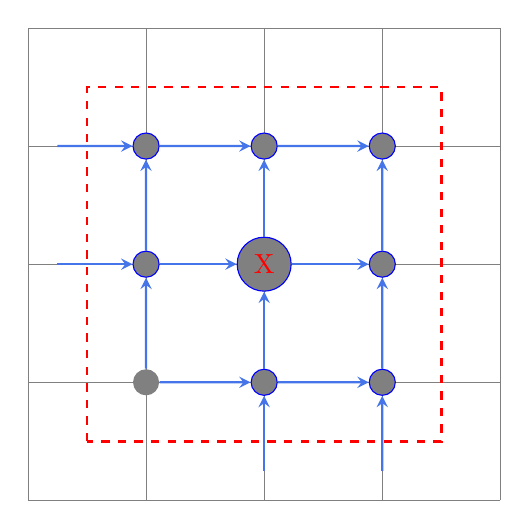
\begin{tikzpicture}[scale=1.5]
            \tikzstyle{model}=[circle,draw=none,fill=gray]
            \tikzstyle{split}=[>=stealth,->,thick, draw=blueind]
            \tikzstyle{merge}=[>=stealth,->,thick, draw=red]
            \draw[step=1cm, help lines] (-2,-2) grid (2,2);
            \node[model] (mode) at (0,0) {{\color{red}X}};

            \draw[color=red, line width=1pt, dashed] (-1.5,-1.5) rectangle ++(3,3);

            \node[model] (bottom_left) at (-1,-1) {};
            \node[model, draw=blue] (row_1) at (0,-1) {};
            \node[model, draw=blue] (col_1) at (-1,0) {};
            \node[model, draw=blue] (row_2) at (1,-1) {};
            \node[model, draw=blue] (col_2) at (-1,1) {};
            \node[model, draw=blue] (mode) at (0,0) {{\color{red}X}};
            \node[model, draw=blue] (row_3) at (1,0) {};
            \node[model, draw=blue] (col_3) at (0,1) {};
            \node[model, draw=blue] (top_right) at (1,1) {};

            \draw[split] (bottom_left) -- (col_1);
            \draw[split] (-1.75,0) -- (col_1);
            \draw[split] (bottom_left) -- (row_1);
            \draw[split] (0,-1.75) -- (row_1);


            \draw[split] (col_1) -- (col_2);
            \draw[split] (-1.75,1) -- (col_2);
            \draw[split] (row_1) -- (row_2);
            \draw[split] (1,-1.75) -- (row_2);
            \draw[split] (row_1) -- (mode);
            \draw[split] (col_1) -- (mode);


            \draw[split] (col_2) -- (col_3);
            \draw[split] (row_2) -- (row_3);
            \draw[split] (mode) -- (row_3);
            \draw[split] (mode) -- (col_3);

            \draw[split] (col_3) -- (top_right);
            \draw[split] (row_3) -- (top_right);
        \end{tikzpicture}
        \caption[forward]{Visualisation of a forward pass of moving window}\label{fig:visualisation-forward-pass}
    \end{subfigure}
    \hfill
    \begin{subfigure}[b]{0.48\textwidth}
        \begin{tikzpicture}[scale=1.5]
            \tikzstyle{model}=[circle,draw=none,fill=gray]
            \tikzstyle{split}=[>=stealth,->,thick, draw=blueind]
            \tikzstyle{merge}=[>=stealth,->,thick, draw=red]
            \draw[step=1cm, help lines] (-2,-2) grid (2,2);
            \draw[color=red, line width=1pt, dashed] (-1.5,-1.5) rectangle ++(3,3);

            \node[model, draw=mypurple] (top_right) at (1,1) {};
            \node[model, draw=mypurple] (row_3) at (1,0) {};
            \node[model, draw=mypurple] (col_3) at (0,1) {};
            \node[model, draw=mypurple] (row_2) at (1,-1) {};
            \node[model, draw=mypurple] (col_2) at (-1,1) {};
            \node[model, draw=mypurple] (mode) at (0,0) {{\color{red}X}};
            \node[model, draw=red] (bottom_left) at (-1,-1) {};
            \node[model, draw=mypurple] (row_1) at (0,-1) {};
            \node[model, draw=mypurple] (col_1) at (-1,0) {};

            \draw[merge] (1,1.75) -- (top_right);
            \draw[merge] (1.75,1) -- (top_right);
            \draw[merge] (0,1.75) -- (col_3);
            \draw[merge] (1.75,0) -- (row_3);
            \draw[merge] (1.75,-1) -- (row_2);
            \draw[merge] (-1,1.75) -- (col_2);

            \draw[merge] (top_right) -- (col_3);
            \draw[merge] (top_right) -- (row_3);
            \draw[merge] (col_3) -- (col_2);
            \draw[merge] (row_3) -- (row_2) ;
            \draw[merge] (row_3) -- (mode);
            \draw[merge] (col_3) -- (mode);
            \draw[merge] (col_2) --(col_1);
            \draw[merge] (row_2) -- (row_1);
            \draw[merge] (mode) -- (row_1);
            \draw[merge] (mode) -- (col_1);
            \draw[merge] (col_1) -- (bottom_left);
            \draw[merge] (row_1) -- (bottom_left);
        \end{tikzpicture}
        \caption[forward]{Visualisation of a backward pass of moving window}\label{fig:visualisation-backward-pass}
    \end{subfigure}
    \caption{Moving window procedure, the center node marked with an {\color{red}X} is the mode of BIC-L}\label{fig:moving-window-procedure}
\end{figure}

\paragraph*{Forward pass} The forward pass consists for a model at $(Q_1, Q_2)$
to compute the possible splits from the block memberships of its ``predecessors``.
The predecessors are the point at the left $(Q_1 - 1, Q_2)$ and below
$(Q_1, Q_2 - 1)$ the current model (if they exist). To update the current model,
we take its predecessors block memberships and try to split one of the blocks in
two. Then the current model is fitted using this clustering as a starting
clustering. Once all the possible splits are fitted, they are compared, keeping
the best, in the sense of the BIC-L. If a model was already present it is also
compared and the best is chosen as the model for this round at $(Q_1, Q_2)$.\\
The procedure then repeats for the point at $(Q_1 + 1, Q_2)$ until it reaches
$(Q_{1,center} + depth, Q_2)$ from which it repeats from
$(Q_{1,center} - depth, Q_2 + 1)$. This repeats until computing the best model
for $(Q_{1,center} + depth, Q_{2,center} + depth)$.
\textit{Note on the initialization:} The forward pass starts from the point
$(Q_{1,center} + depth, Q_{2,center} + depth)$, so this points needs to have at
least a model fitted. In the best case, the greedy exploration will have visited
this point. But if the point has not been visited, a model will be fitted from
a spectral initialization (i.e the block memberships is computed by using a
spectral clustering). From this point, the next model will have at least one
predecessor and the procedure can iterate.

\paragraph*{Backward pass} The backward pass consists for a model at $(Q_1, Q_2)$
to compute the possible merges from the block memberships of its ``predecessors``.
The predecessors are the point at the right $(Q_1 + 1, Q_2)$ and on top
$(Q_1, Q_2 + 1)$ of the current model (if the predecessors exist). To update the
current model, we take its predecessors block memberships and try to merge two
blocks in one. Then the current model is fitted using this clustering as
a starting clustering. Once all the possible merges are fitted, they are
compared, keeping the best, in the sense of the BIC-L.
If a model was already present it is also
compared and the best is chosen as the model for this round at $(Q_1, Q_2)$.\\
The procedure then repeats for the point at $(Q_1 - 1, Q_2)$ until it reaches
$(Q_{1,center} - depth, Q_2)$ from which it repeats from
$(Q_{1,center} - depth, Q_2 - 1)$. This repeats until computing the best model
for ($Q_{1,center} - depth, Q_{2,center} - depth$).
\textit{Note on the initialization:} The backward pass starts from
$(Q_{1,center} + depth, Q_{2,center} + depth)$, we know it was initialized at
least by the forward pass, no special case here.\\

At the end of the moving window pass, the model of max BIC-L is the new best
fit and the procedure can repeat until convergence.

\section{Networks clustering}
\label{sec:networks-clustering}
As in~\cite{chabert-liddellLearningCommonStructures2023} we use a recursive
algorithm to determine the best clustering of the given networks. The procedure
being the same, we will present it briefly and focus on adjustments.

When networks in a collection do not share the same mesoscale connectivity
structure we want to be able to partition them correctly. For this we perform
a clustering of networks.

The process of clustering a collection of networks involves discovering a
partition $\mathcal{G} = (\mathcal{M}_g)_{g=1,\dots,G}$ of $\{1,\dots, M\}$.
Given $\mathcal{G}$ we set the following model on $\bm{X}$:

\[
    \forall g \in \{1,\dots, G\}, \forall m \in \mathcal{M}_g, X^m \sim \mathcal{F}\text{-}BiSBM(Q_1^g, Q_2^g, \bm{\pi^m, \rho^m,} \bm{\alpha}^g)
\]

And we defined the score of a given partition $\mathcal{G}$:
\[
    Sc(\mathcal{G}) = \sum_{g=1}^{G} \max_{Q^g=1,\dots,Q_{\max}} \text{BIC-L}((X^m)_{m\in\mathcal{M}_g},Q_1^g, Q_2^g)
\]
Thus the score consists of the sum of the BIC-L of the sub-collections for the
partition $\mathcal{G}$.

\subsection{Dissimilarity between two networks}
\label{ssec:dissimilarity-between-two-networks}
The parameters for the dissimilarity are defined as follow:
\begin{align*}
    \widetilde{n}_{qr}^m = \sum_{i=1}^{n_1^m} \sum_{j=1}^{n_2^m} \widehat{\tau}_{iq}^{1,m} \widehat{\tau}_{jr}^{2,m},
    && \widetilde{\alpha}_{qr}^m = \frac{\sum_{i=1}^{n_1^m} \sum_{j=1}^{n_2^m} \widehat{\tau}_{iq}^{1,m} \widehat{\tau}_{jr}^{2,m} X_{ij}^m}{\widetilde{n}_{qr}^m},\\
    \widetilde{\pi}_q^m = \frac{\sum_{i=1}^{n_1^m} \widehat{\tau}_{iq}^{1,m}}{n_1^m},
    && \widetilde{\rho}_r^m = \frac{\sum_{j=1}^{n_2^m} \widehat{\tau_{jr}}^{2,m}}{n_2^m}
\end{align*}
And the dissimilarity between any pair of networks $(m,m')\in\mathcal{M}^2$ is then:
\[
    D_{\mathcal{M}}(m,m') = \sum_{q = 1}^{Q_1} \sum_{r = 1}^{Q_2} \max(\widetilde{\pi}_{q}^{m}, \widetilde{\pi}_{q}^{m'}) \left( \widetilde{\alpha}_{qr}^{m} - \widetilde{\alpha}_{qr}^{m'}\right)^{2} \max(\widetilde{\rho}_{r}^{m}, \widetilde{\rho}_{r}^{m'})
\]

\begin{figure}[H]
    \centering
    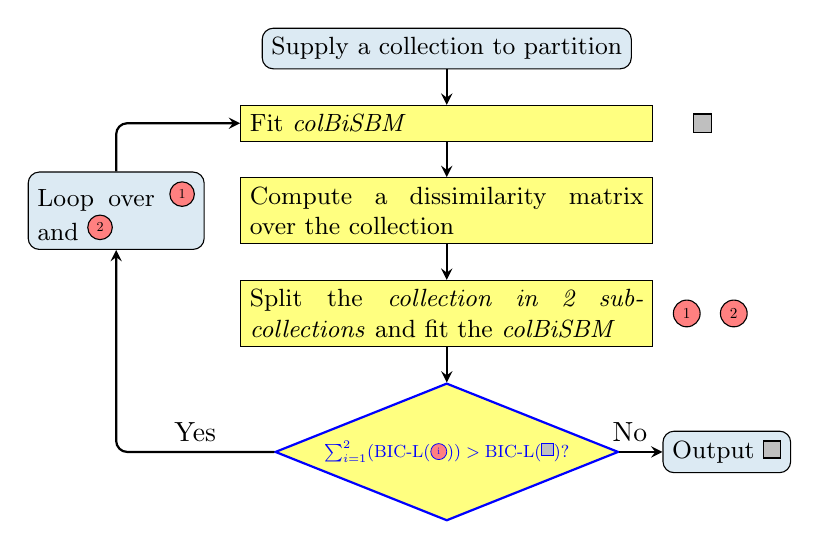
\begin{tikzpicture}
        \tikzstyle{instruct}=[font=\small, text justified, rectangle,draw,fill=yellow!50]
        \tikzstyle{first_col}=[rectangle, text justified, draw,fill=gray!50]
        \tikzstyle{second_col}=[scale=0.55, circle, draw,fill=red!50]
        \tikzstyle{test}=[font=\small, text justified, diamond, aspect=2.5,thick,
        draw=blue,fill=yellow!50,text=blue]
        \tikzstyle{es}=[font=\small, text justified, rectangle,draw,rounded corners=4pt,fill=cyanind!25]

        \node[es] (liste) at (0,4) {Supply a collection to partition};
        \node[instruct, text width=5cm, below = 0.45cm of liste] (1-collection) {Fit \emph{colBiSBM}};
        \node[first_col, right = 0.5cm of 1-collection] (1-col-obj) {};
        \node[instruct, text width=5cm, below = 0.45cm of 1-collection] (dissimi) {Compute a dissimilarity matrix over the collection};
        \node[instruct, text width=5cm, below = 0.45cm of dissimi] (2-sous-collection) {Split the \emph{collection in 2 sub-collections} and fit the \emph{colBiSBM}};
        \node[second_col, right = 0.25cm of 2-sous-collection] (1-sec-col-obj) {1};
        \node[second_col, right = 0.25cm of 1-sec-col-obj] (1-sec-col-obj) {2};
        \node[test,below = 0.45cm of 2-sous-collection, scale=0.7] (BICL-test) {$\sum_{i=1}^{2} (\text{BIC-L}(\tikz[baseline=-0.25cm]{\node[second_col] {i};} )) > \text{BIC-L}(\tikz[baseline=-0.25cm]{\node[first_col] {};})$?};
        \node[es, right = 0.55cm of BICL-test] (sortie) {Output \tikz{\node[rectangle, draw, fill=gray!50, rounded corners=0pt] {};}};
        \node[es, left = 0.45cm of dissimi, text width = 2cm] (recursion) {Loop over \tikz{\node[second_col] {1};} and \tikz{\node[second_col] {2};} };

        \tikzstyle{suite}=[->,>=stealth,thick,rounded corners=4pt]
        \draw[suite] (liste) -- (1-collection);
        \draw[suite] (1-collection) -- (dissimi);
        \draw[suite] (dissimi) -- (2-sous-collection);
        \draw[suite] (2-sous-collection) -- (BICL-test);
        \draw[suite] (BICL-test) -| node[near start, above, fill=none] {Yes} (recursion);
        \draw[suite] (recursion.north) |- (1-collection.west);
        \draw[suite] (BICL-test) -- node[near start, above, fill=none] {No} (sortie);
    \end{tikzpicture}
    \caption{Network clustering procedure}
    \label{fig:netclustering-procedure}
\end{figure}

The above figure (\ref{fig:netclustering-procedure}) shows a condensed
explanation of the network clustering algorithm.

The idea is to adjust the \emph{colBiSBM} model over the full collection of $M$
networks and then compute the dissimilarity matrix between all networks of the
collection. We obtain the collection $\mathcal{G} = \{\mathcal{M}\}$ the trivial
partition in a unique group.

Then using the \emph{Kmeans} we split the collection in two sub-collections with
the dissimilarity matrix. The two sub-collections are fitted and we compute
the score of this new partition $\mathcal{G}^{*} = \{G_1, G_2\}$.

If $Sc(\mathcal{G}^{*}) > Sc(\mathcal{G})$ then we repeat the same procedure on
$G_1$ and $G_2$. Else we return $\mathcal{G}$.

We illustrate our capacity to perform a partition of a collection for all
colBiSBM models in \ref{sec:network-clustering-of-simulated-networks}.

\chapter{Simulation studies}\label{chap:simulation-studies}
\section{Network clustering of simulated networks}\label{sec:network-clustering-of-simulated-networks}

\chapter{Applications}
\hypertarget{application-to-data}{%
\section{\texorpdfstring{Application to
\cite{doreRelativeEffectsAnthropogenic2021}
data}{Application to  data}}\label{application-to-data}}

\label{sec:application-to-dorerelativeeffectsanthropogenic2021-data}

% \hypertarget{application-to-data}{%
\section{\texorpdfstring{Application to
\cite{doreRelativeEffectsAnthropogenic2021}
data}{Application to  data}}\label{application-to-data}}

\label{sec:application-to-dorerelativeeffectsanthropogenic2021-data}

\hypertarget{clustering-with-model-iid}{%
\subsection{Clustering with model iid}\label{clustering-with-model-iid}}

With the \emph{iid-colBiSBM} we obtain 5 collections with the following
structures:

\subsubsection{Pour la collection 1 }

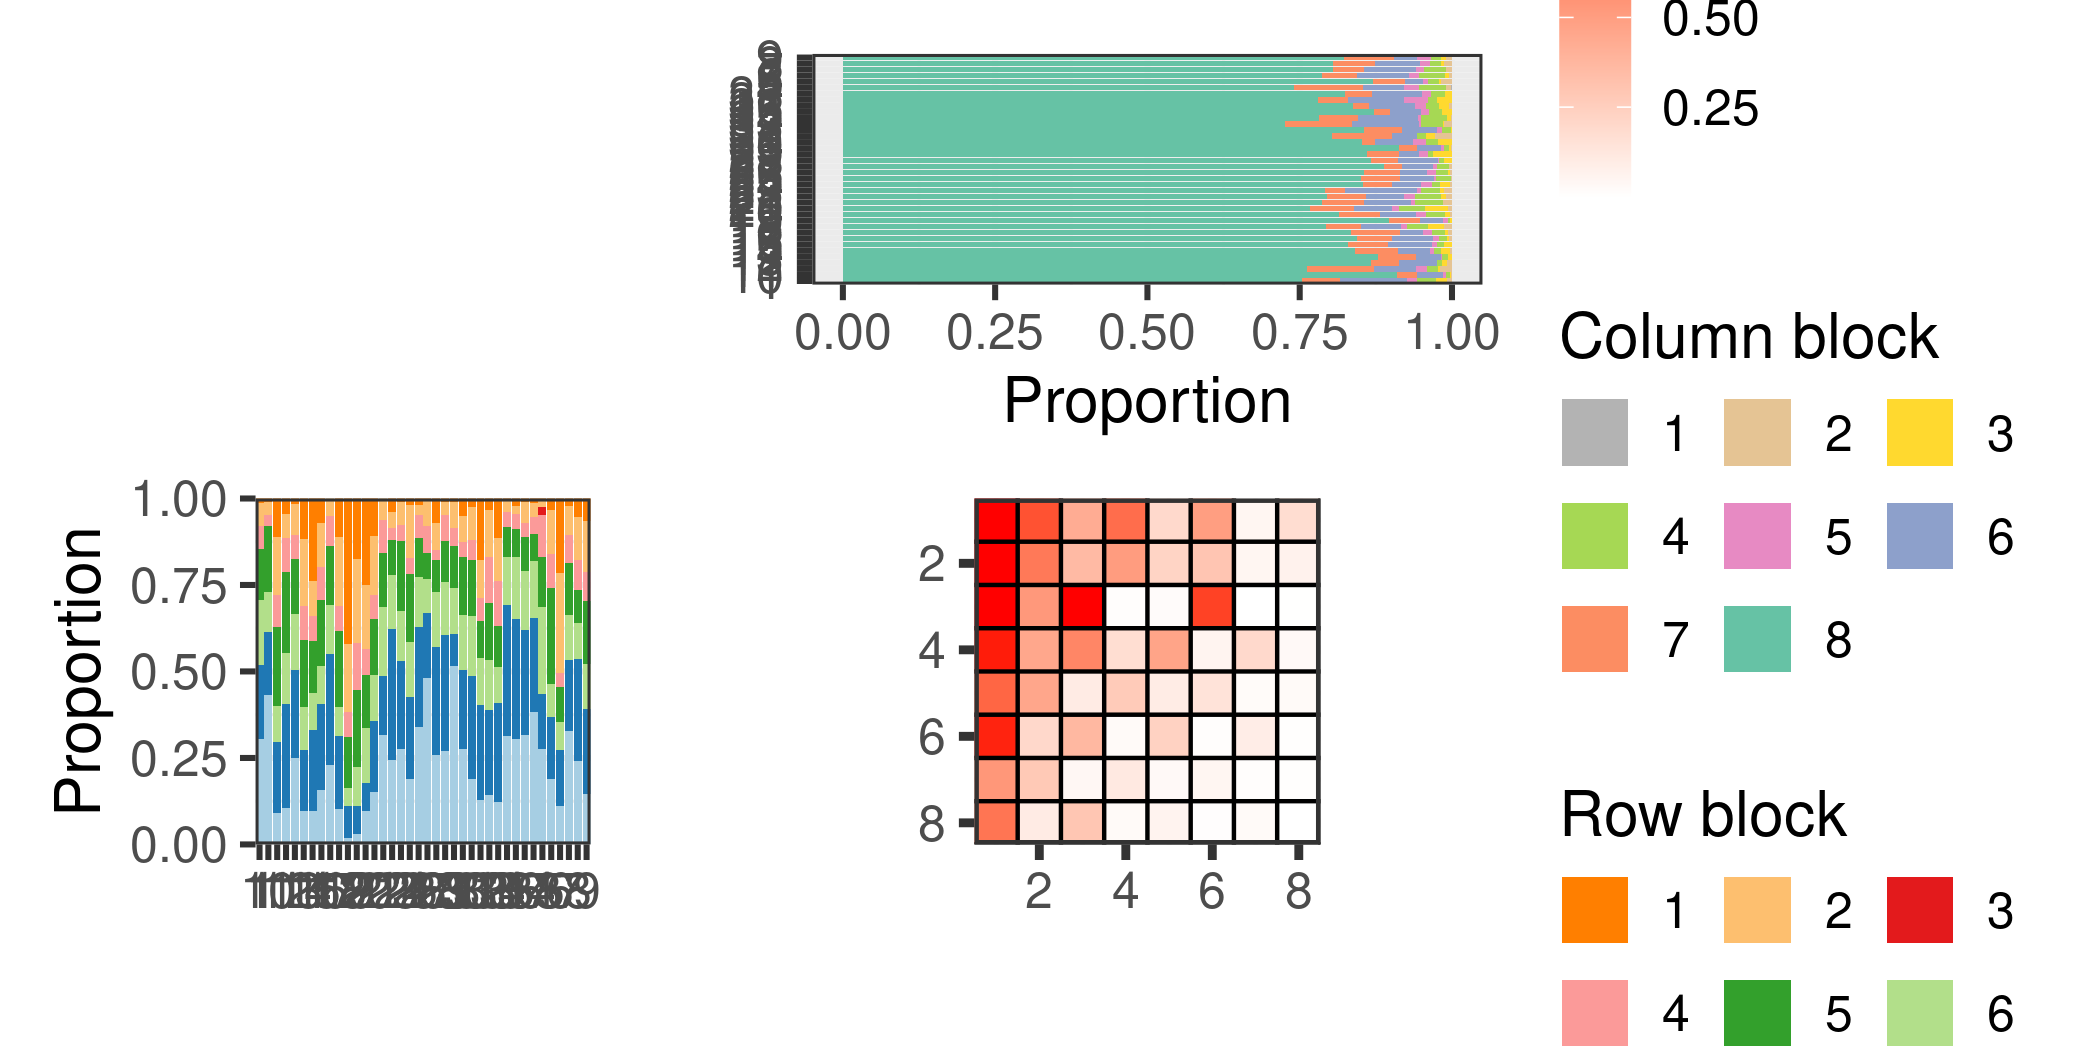
\includegraphics{./img/4c7e9819bb707372d35035947dfe7848b594b688.png}\newline \tiny

\begin{tabular}{l}
\toprule
Networks\\
\midrule
arroyo1982\_1+arroyo1982\_2+arroyo3\\
eberling1999\\
kato1990\\
petanidou1991\\
Junker2013\\
\addlinespace
bartomeus2008\\
Benadi2013\_1(950m)+Benadi2013\_2(1170m)+Benadi2013\_6(2020m)\\
Benadi2013\_4(1700m)+Benadi2013\_5(1800m)\\
Struck1994\\
Kato2000\\
\addlinespace
Albrecht2010\_49yr+Albrecht2010\_63yr+Albrecht2010\_84yr+Albrecht2010\_109yr+Albrecht2010\_130yr\\
Baldock2011\_TB+Baldock2011\_JN\\
Dattilo2016\\
Devoto2005\_PP+Devoto2005\_AP\\
Devoto2005\_VT\\
\addlinespace
Devoto2005\_LL+Devoto2005\_CT\\
Freitas2006\\
Gibson2006\_TA2\\
Jedrzejewska2013\_Ochata+Jedrzejewska2013\_Kabaty\\
MonteroCastano2017\_Albufera+MonteroCastano2017\_Llimpa+MonteroCastano2017\_Tirant\\
\addlinespace
Kehinde2014\_Joostenberg\_Conv+Kehinde2014\_Joostenberg\_Org+Kehinde2014\_Joostenberg\_Nat+Kehinde2014\_Laibach\_Conv+Kehinde2014\_Laibach\_Org+Kehinde2014\_Laibach\_Nat+Kehinde2014\_Spier\_Conv+Kehinde2014\_Spier\_Nat\\
Pinheiro2008\\
Watts2016\_Chicon+Watts2016\_Mantanay+Watts2016\_Choquebamba+Watts2016\_Huaran+Watts2016\_Piscacucho+Watts2016\_Poques+Watts2016\_Pumamarca+Watts2016\_Tiaparo+Watts2016\_Yanacocha\\
Kato1993\\
KatoMiura1996\\
\addlinespace
Kakutani1990\\
Inoue1990\\
Fragoso\_RA2+Fragoso\_RA3+Fragoso\_RD1+Fragoso\_RD3\\
Souza\_cerrado\\
Souza\_chaco\\
\addlinespace
Souza\_pantanal\\
Souza\_vereda\\
Adedoja2019\\
Oleques2019\\
Baldock2019\_Bristol\\
\addlinespace
Baldock2019\_Edinburgh\\
Baldock2019\_Leeds\\
Baldock2019\_Reading\\
\bottomrule
\end{tabular}

\normalsize\newline\[\begin{pmatrix} 1 &0.83 &0.43 &0.73 &0.2 &0.5 &0.05 &0.18 \\1 &0.67 &0.36 &0.51 &0.22 &0.3 &0.05 &0.07 \\1 &0.53 &1 &0.01 &0.02 &0.89 &0 &0 \\0.97 &0.45 &0.62 &0.18 &0.47 &0.06 &0.2 &0.03 \\0.76 &0.46 &0.1 &0.27 &0.1 &0.14 &0.02 &0.03 \\0.96 &0.2 &0.37 &0.03 &0.24 &0.01 &0.09 &0.01 \\0.54 &0.28 &0.04 &0.12 &0.03 &0.05 &0.01 &0.01 \\0.69 &0.1 &0.3 &0.02 &0.06 &0.01 &0.03 &0 \\ \end{pmatrix}\]

\subsubsection{Pour la collection 2 }

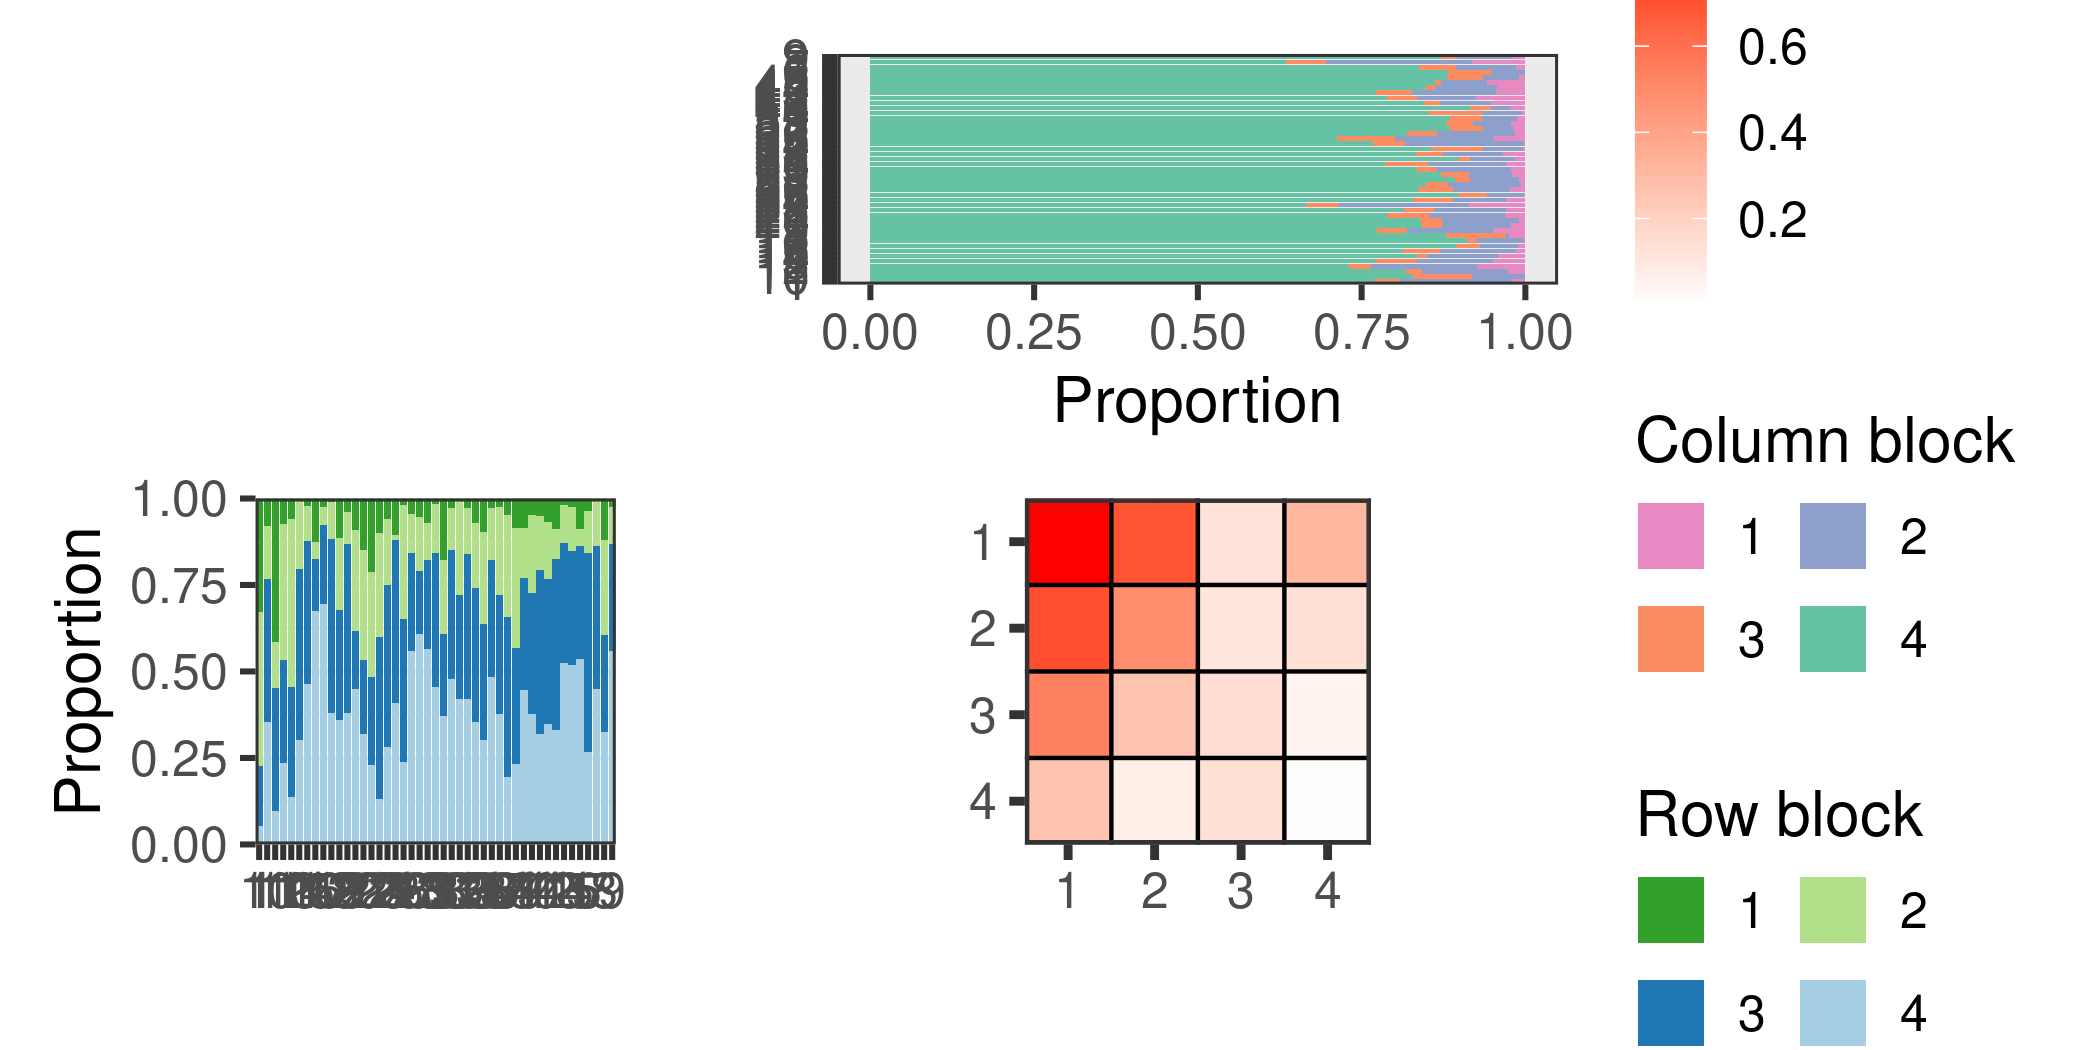
\includegraphics{./img/2e1295ef8143b9413e953a4c0c2da20d962158f6.png}\newline \tiny

\begin{tabular}{l}
\toprule
Networks\\
\midrule
dupont2003\\
herrera1988\\
inouye1988\\
medan2002ld\\
medan2002rb\\
\addlinespace
ramirez1992\\
ramirez1989\\
Burkle2013\\
Olito-Fox2014\\
Benadi2013\_3(1340m)\\
\addlinespace
Aizen2008\_Challhuaco\_U+Aizen2008\_Challhuaco\_D\\
Aizen2008\_Cerro Otto\_U+Aizen2008\_Cerro Otto\_D\\
Aizen2008\_Llao-llao\_U+Aizen2008\_Llao-llao\_D\\
Chamberlain\_cr1+Chamberlain\_cr2+Chamberlain\_fs1+Chamberlain\_fs2+Chamberlain\_go1+Chamberlain\_go2+Chamberlain\_mm1+Chamberlain\_mm2+Chamberlain\_mz1+Chamberlain\_mz2+Chamberlain\_sm1+Chamberlain\_sm2\\
Chamberlain\_HLU+Chamberlain\_HLG+Chamberlain\_OKU+Chamberlain\_OKG+Chamberlain\_WLU+Chamberlain\_WLG+Chamberlain\_SOU+Chamberlain\_SOG\\
\addlinespace
Devoto2005\_LQ\\
Devoto2005\_LT+Devoto2005\_LH\\
LemusJimenez2003\\
Lundgren2005\\
Marrero2013\\
\addlinespace
Trojelsgaard2015\_La Gomera\\
Trojelsgaard2015\_Gran Canaria\\
Zackenberg\\
Yoshihara2008\\
Fragoso\_RA1+Fragoso\_RD2\\
\addlinespace
PopicThesis\\
Pornon2017\\
Orford\_B1+Orford\_B2+Orford\_B3+Orford\_B4+Orford\_B5+Orford\_B10\\
Orford\_B6+Orford\_B7+Orford\_B8+Orford\_B9\\
Blumel2016\\
\addlinespace
Kantsa2018\\
Bennett2018\\
Adedoja2018b\_baseZone+Adedoja2018b\_MidZone+Adedoja2018b\_HighZone+Adedoja2018b\_PeakZone\\
CordenizPicanco2018\_NatVeg\\
CordenizPicanco2018\_ExoFor\\
\addlinespace
Benadi2018\\
Hackett2019\_NZ\_salt\_marsh+Hackett2019\_NZ\_sand\_dune+Hackett2019\_NZ\_scrub\_coprosma\\
Jolls2019\\
Traveset2013\_Fernandina\\
Traveset2013\_Pinta\\
\addlinespace
Traveset2013\_Santiago\\
Traveset2013\_SantaCruz\\
Traveset2013\_SanCristobal\\
Simanonok2014\\
Son2019\_a1+Son2019\_a2+Son2019\_a3+Son2019\_a4+Son2019\_a5+Son2019\_a6+Son2019\_a7+Son2019\_a8+Son2019\_F1+Son2019\_F2+Son2019\_F3+Son2019\_F4+Son2019\_F5+Son2019\_F6+Son2019\_F7+Son2019\_F8\\
\bottomrule
\end{tabular}

\normalsize\newline\[\begin{pmatrix} 0.84 &0.69 &0.13 &0.32 \\0.71 &0.49 &0.11 &0.14 \\0.54 &0.26 &0.14 &0.05 \\0.26 &0.07 &0.14 &0.01 \\ \end{pmatrix}\]

\subsubsection{Pour la collection 3 }

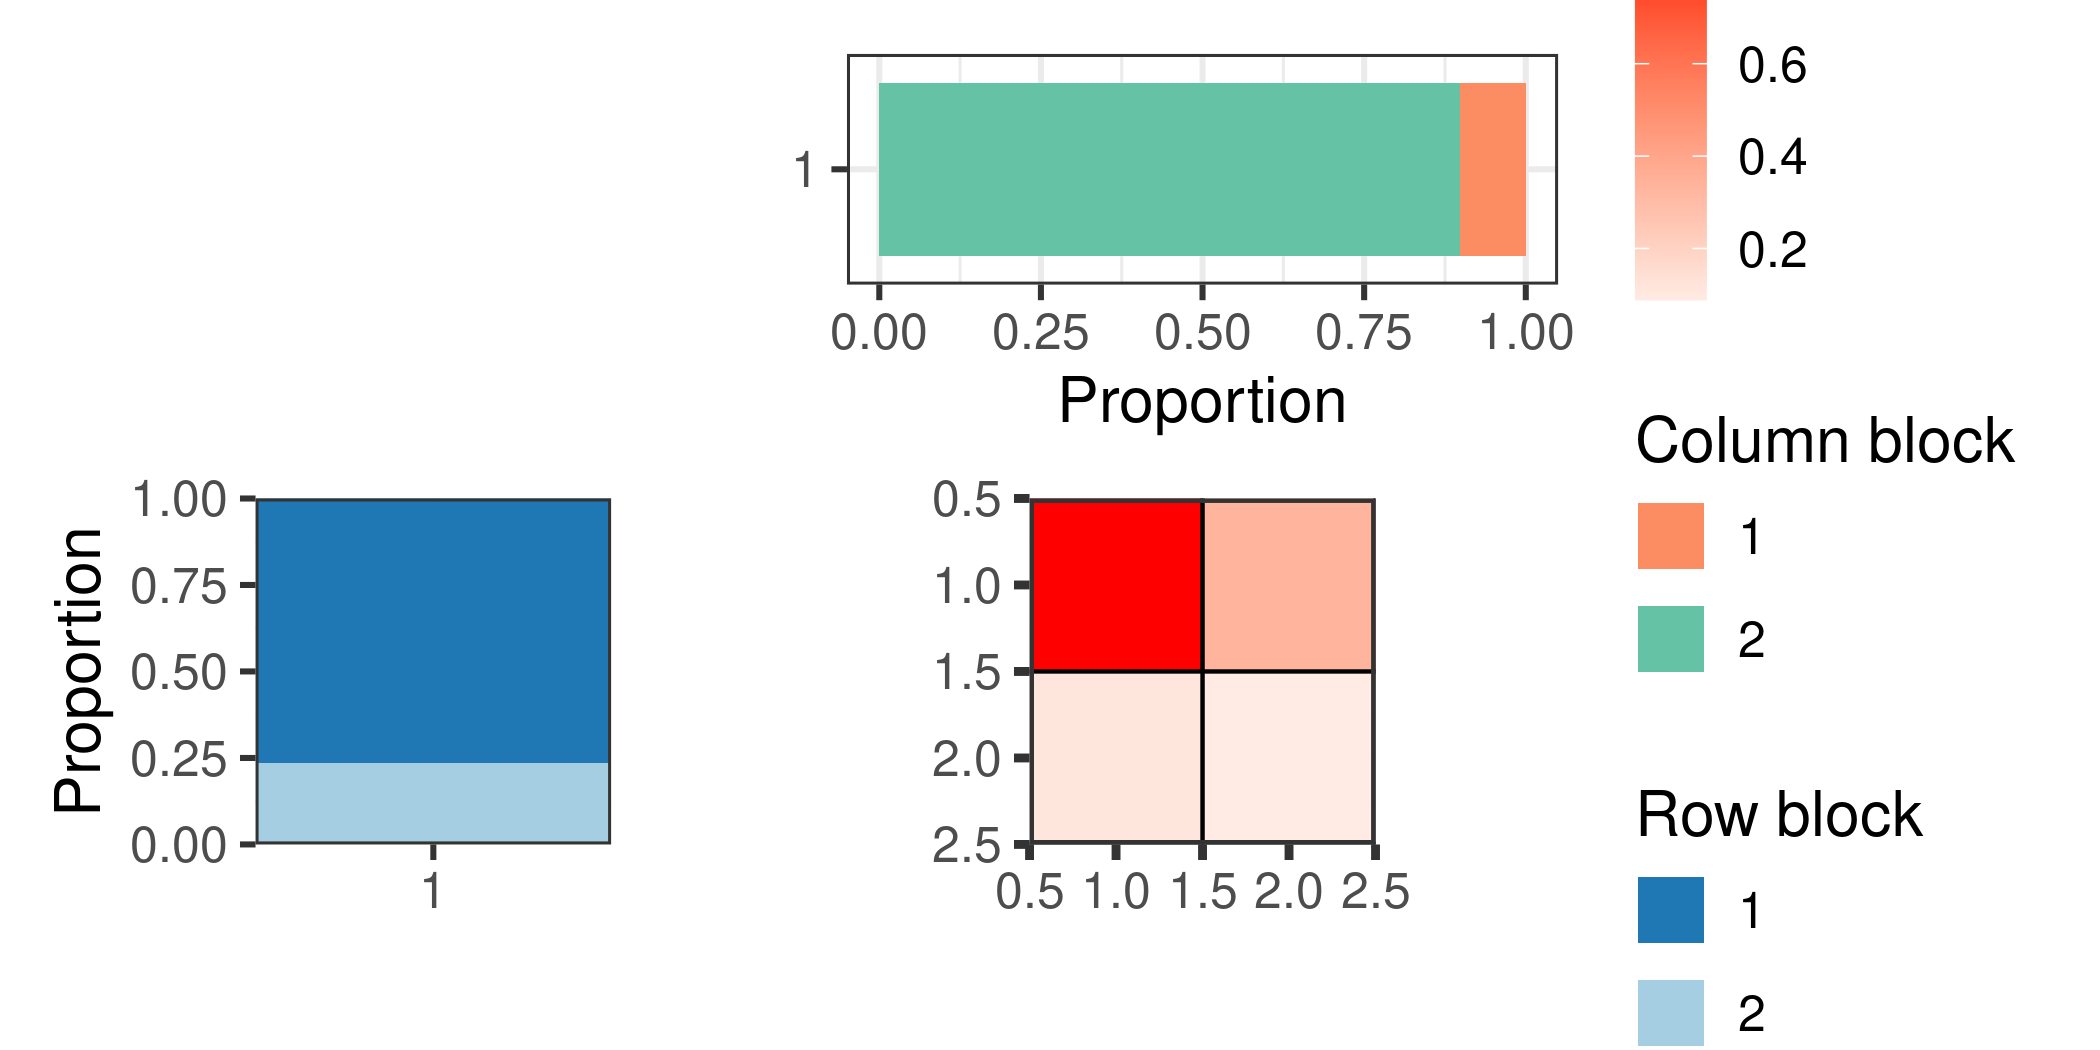
\includegraphics{./img/e69b18419936d1e08301cce4cb1c78acba2044c4.png}\newline \tiny

\begin{tabular}{l}
\toprule
Networks\\
\midrule
small1976\\
\bottomrule
\end{tabular}

\normalsize\newline\[\begin{pmatrix} 0.87 &0.33 \\0.11 &0.09 \\ \end{pmatrix}\]

\subsubsection{Pour la collection 4 }

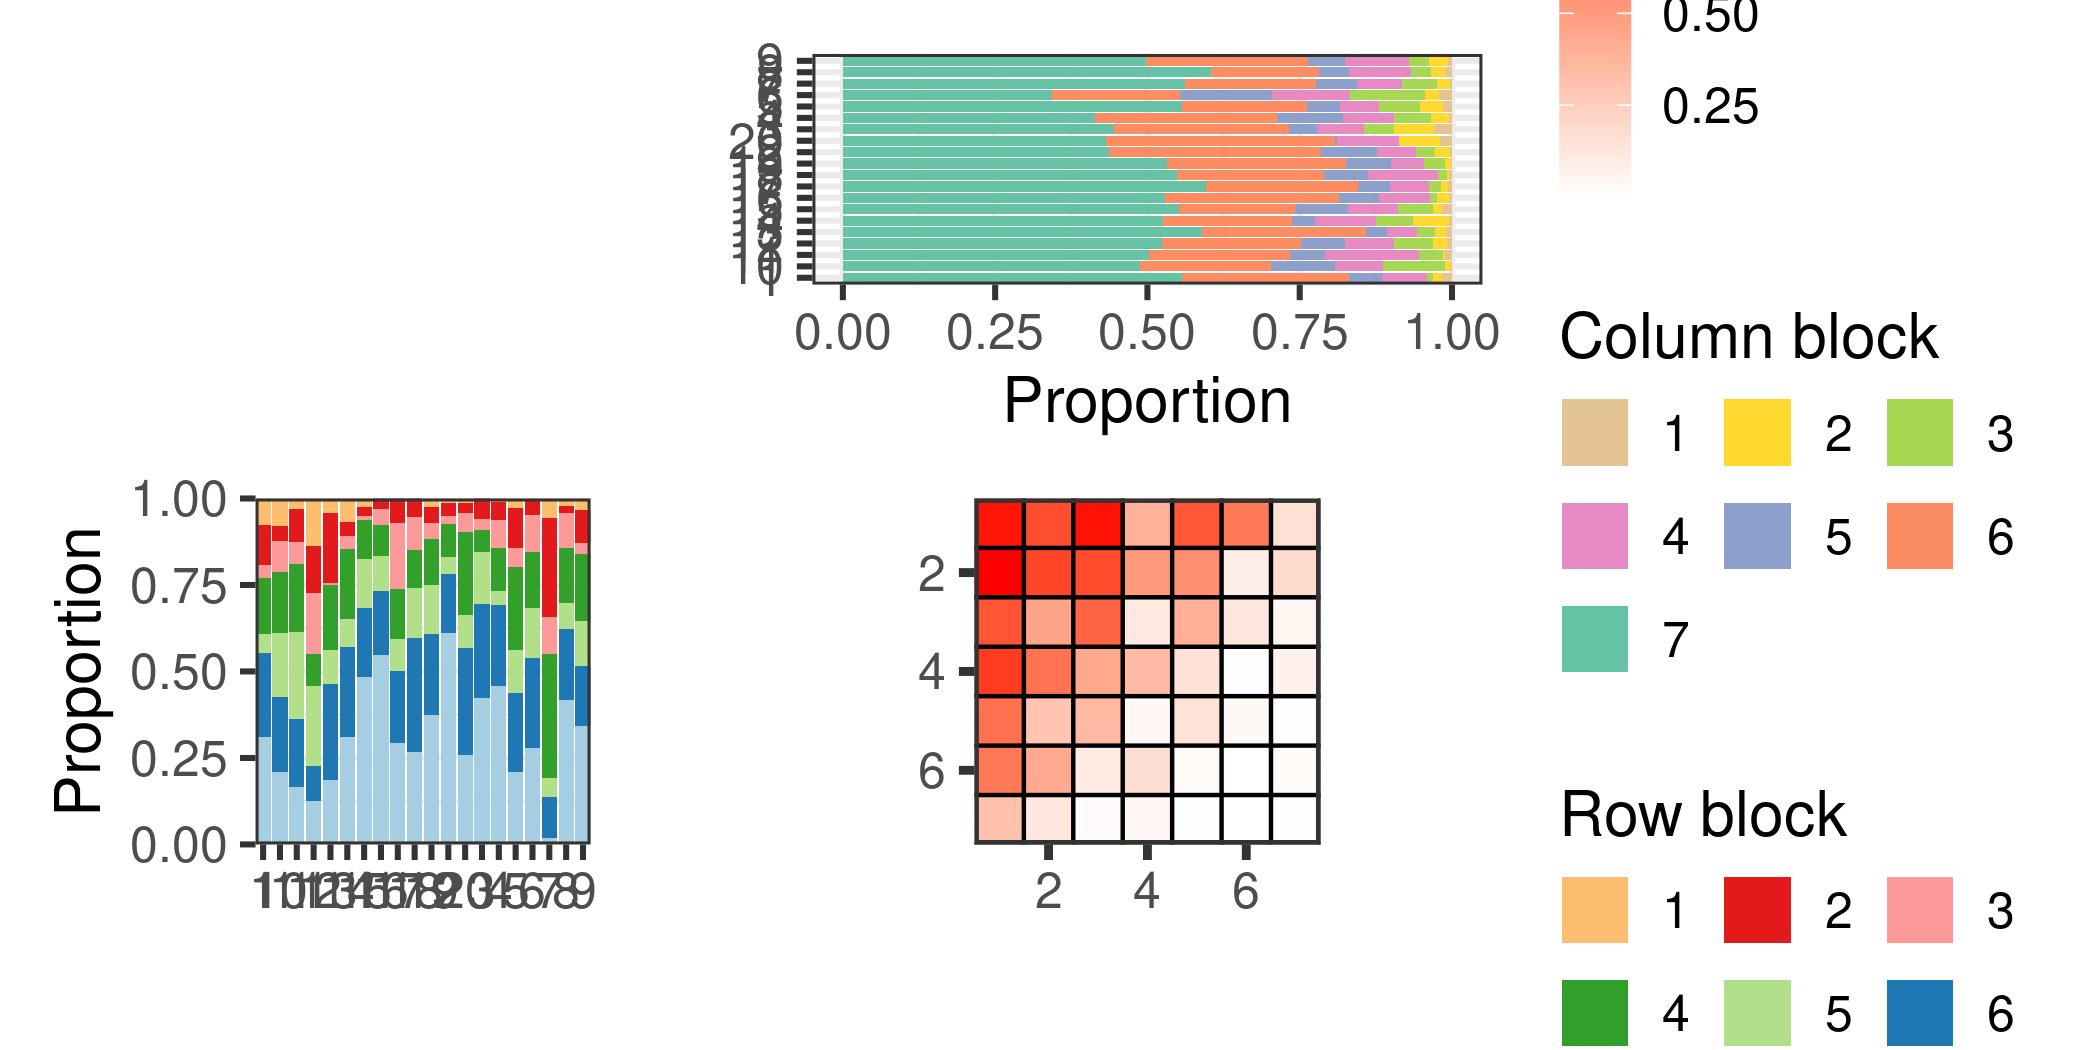
\includegraphics{./img/c1e07feffa95efd0355d15ccfec6dff687c1ef88.png}\newline \tiny

\begin{tabular}{l}
\toprule
Networks\\
\midrule
smith-ramirez2005\\
Weiner2011\\
Kaiser\_control+Kaiser\_restored\\
Gilarranz2014\_amarante+Gilarranz2014\_barrosa+Gilarranz2014\_cincocerros+Gilarranz2014\_difuntito+Gilarranz2014\_difuntos+Gilarranz2014\_elmorro+Gilarranz2014\_labrava+Gilarranz2014\_lachata+Gilarranz2014\_lapaja+Gilarranz2014\_piedraalta+Gilarranz2014\_vigilancia+Gilarranz2014\_volcan\\
Kaiser-Bunbury2017\_Bernica+Kaiser-Bunbury2017\_Casse-dent+Kaiser-Bunbury2017\_Copolia+Kaiser-Bunbury2017\_La-Reserve+Kaiser-Bunbury2017\_Rosebelle+Kaiser-Bunbury2017\_Salazie+Kaiser-Bunbury2017\_Tea-Plantation+Kaiser-Bunbury2017\_Trois-Freres\\
\addlinespace
Fang2012\\
Aizen2008\_Puerto Blest\_U+Aizen2008\_Puerto Blest\_D\\
Chamberlain\_Site1+Chamberlain\_Site2+Chamberlain\_Site3+Chamberlain\_Site4+Chamberlain\_Site5+Chamberlain\_Site6\\
Dupont2009\_IsenBjerg+Dupont2009\_Other\\
Gibson2006\_GA1\\
\addlinespace
Gibson2006\_TA1\\
LaraRomero2016\_pe?alara\_EP+LaraRomero2016\_pe?alara\_PA+LaraRomero2016\_nevero\_EP+LaraRomero2016\_nevero\_PA\\
Trojelsgaard2015\_Tenerife Teno Bajo+Trojelsgaard2015\_Tenerife Fasnia\\
Vanbergen2013\_balfarm+Vanbergen2013\_bridgend+Vanbergen2013\_dalhaikie+Vanbergen2013\_netherton+Vanbergen2013\_backhill+Vanbergen2013\_corntulloch+Vanbergen2013\_allancreich\\
Pfeiffer\_CNE+Pfeiffer\_CNM+Pfeiffer\_CNT+Pfeiffer\_CPB+Pfeiffer\_CPM+Pfeiffer\_CPR+Pfeiffer\_CPS+Pfeiffer\_M2+Pfeiffer\_RP1+Pfeiffer\_RP2+Pfeiffer\_LM+Pfeiffer\_LO+Pfeiffer\_BD+Pfeiffer\_BH+Pfeiffer\_BS\\
\addlinespace
Carstensen\_Gigante+Carstensen\_Paulino+Carstensen\_Tinkerbell+Carstensen\_Midway+Carstensen\_Cedro+Carstensen\_Elefante+Carstensen\_Soizig\\
Welti\_ID+Welti\_K1B+Welti\_K4A+Welti\_4B+Welti\_20B+Welti\_20C+Welti\_N1A+Welti\_N1B+Welti\_N4A+Welti\_N4B+Welti\_N20A+Welti\_N20B\\
Grass2013\_1+Grass2013\_2+Grass2013\_3+Grass2013\_4+Grass2013\_5+Grass2013\_6+Grass2013\_7+Grass2013\_8+Grass2013\_9+Grass2013\_10+Grass2013\_11+Grass2013\_12+Grass2013\_13+Grass2013\_14+Grass2013\_15+Grass2013\_16+Grass2013\_17\\
Hackett2019\_UK\_sand\_dune+Hackett2019\_UK\_grassland+Hackett2019\_UK\_heathland+Hackett2019\_UK\_woodland+Hackett2019\_UK\_salt\_marsh+Hackett2019\_UK\_scrub\\
Neli2014\\
\bottomrule
\end{tabular}

\normalsize\newline\[\begin{pmatrix} 0.96 &0.83 &0.96 &0.39 &0.8 &0.16 &0.66 \\0.98 &0.86 &0.83 &0.51 &0.56 &0.19 &0.09 \\0.8 &0.46 &0.74 &0.12 &0.4 &0.05 &0.13 \\0.89 &0.69 &0.44 &0.35 &0.15 &0.07 &0.01 \\0.7 &0.29 &0.35 &0.03 &0.15 &0.01 &0.03 \\0.66 &0.43 &0.1 &0.17 &0.03 &0.02 &0 \\0.32 &0.12 &0.02 &0.04 &0 &0 &0 \\ \end{pmatrix}\]

\subsubsection{Pour la collection 5 }

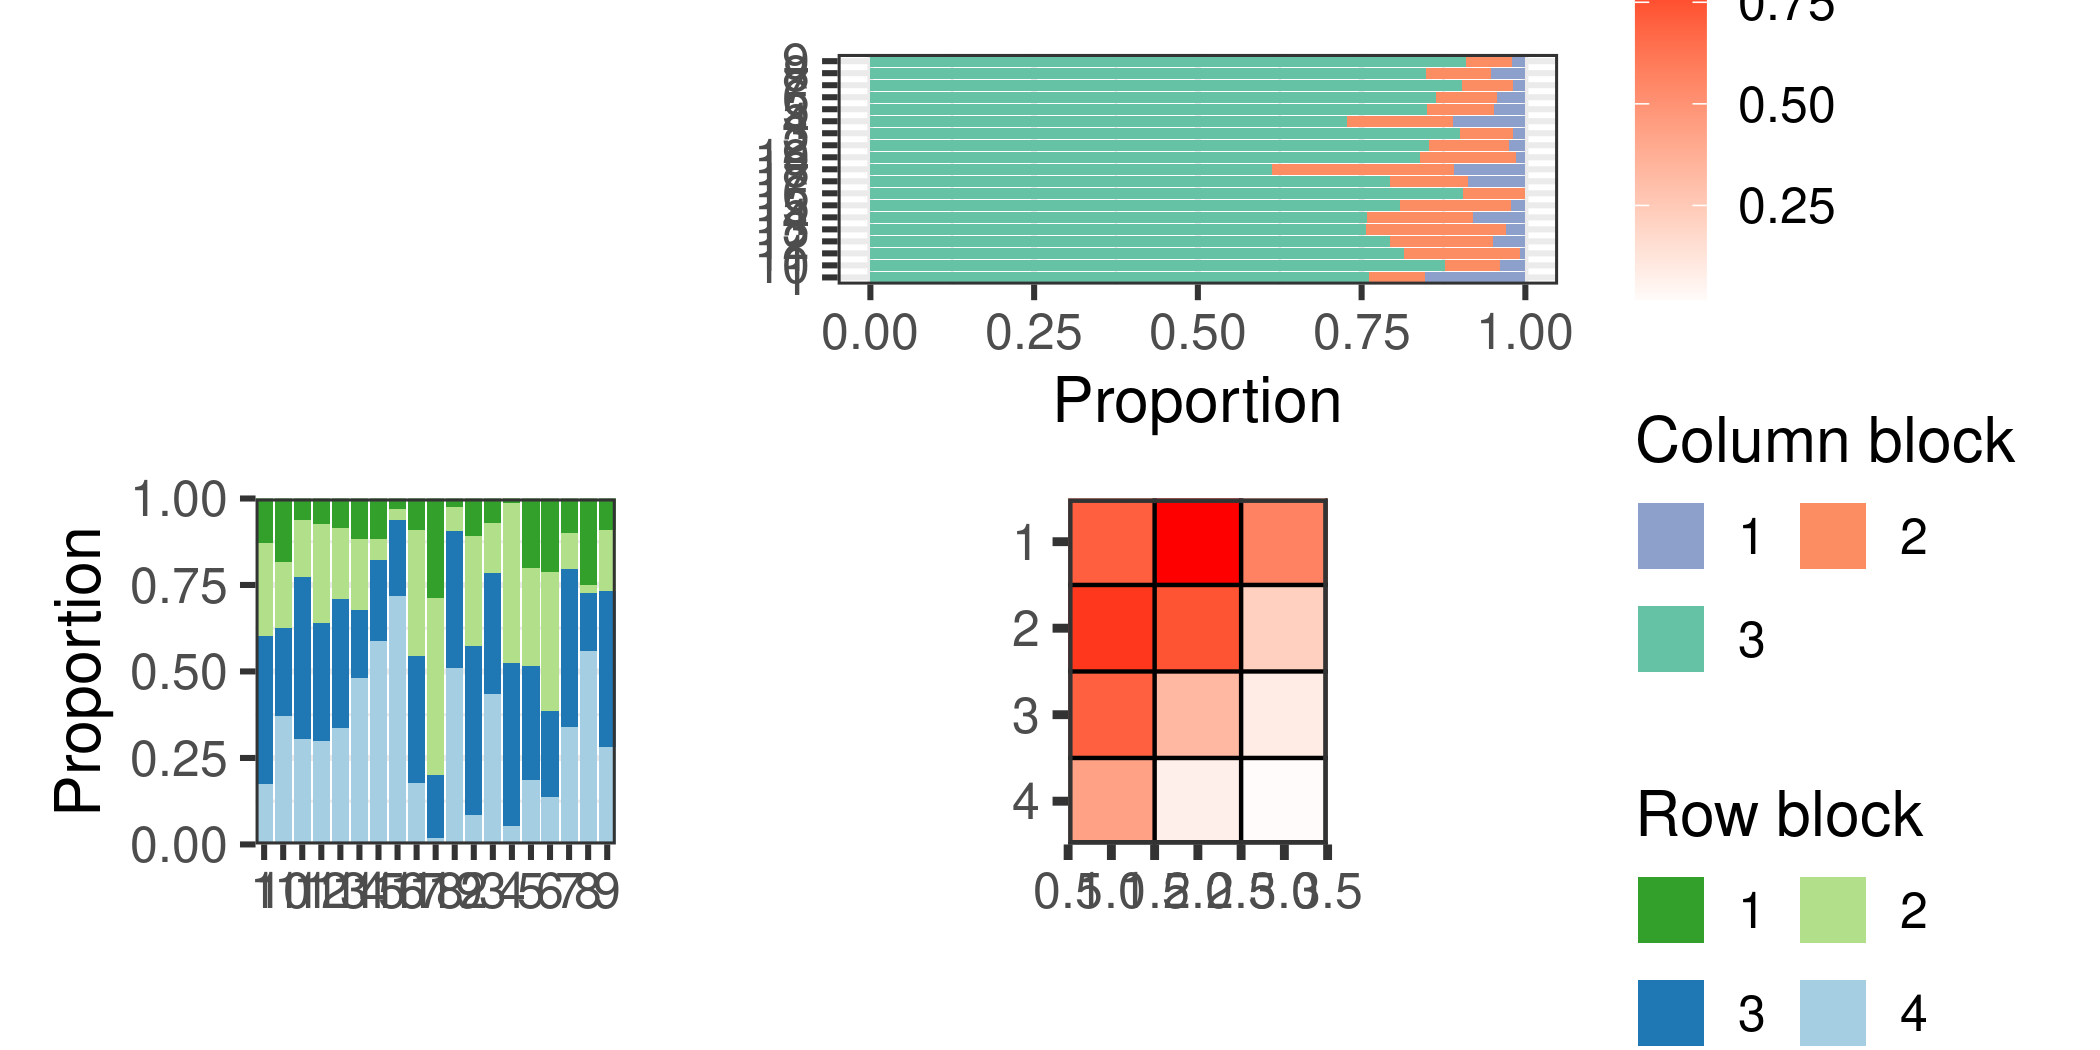
\includegraphics{./img/be6eb1cef4cfa33f60e7f12e0d81b62fb4805328.png}\newline \tiny

\begin{tabular}{l}
\toprule
Networks\\
\midrule
olensen2002aig\\
olensen2002flo\\
vazquez2002\\
Shay2016\\
Gibson2006\_GA2\\
\addlinespace
Gibson2006\_SG\\
Trojelsgaard2015\_El Hierro\\
Trojelsgaard2015\_Fuerteventura\\
Trojelsgaard2015\_Western Sahara\\
Robinson2018\\
\addlinespace
CordenizPicanco2018\_NatFor\\
CordenizPicanco2018\_SemiPast\\
CordenizPicanco2018\_IntPast\\
Biella2019\\
Nel2017\\
\addlinespace
Villalobos2019\\
LaraRomero2019\_blanca+LaraRomero2019\_rajada+LaraRomero2019\_refugio+LaraRomero2019\_torre\\
Ferrero2013\\
Sritongchuay2019\_near+Sritongchuay2019\_far\\
\bottomrule
\end{tabular}

\normalsize\newline\[\begin{pmatrix} 0.71 &0.9 &0.57 &0.83 \\0.74 &0.22 &0.7 &0.33 \\0.09 &0.44 &0.07 &0.02 \\ \end{pmatrix}\]

Et voici donc les valeurs numériques pour les \(\alpha\) (paramètres de
connectivité).

Pour la collection 1 :
\[\begin{pmatrix} 1 &0.83 &0.43 &0.73 &0.2 &0.5 &0.05 &0.18 \\1 &0.67 &0.36 &0.51 &0.22 &0.3 &0.05 &0.07 \\1 &0.53 &1 &0.01 &0.02 &0.89 &0 &0 \\0.97 &0.45 &0.62 &0.18 &0.47 &0.06 &0.2 &0.03 \\0.76 &0.46 &0.1 &0.27 &0.1 &0.14 &0.02 &0.03 \\0.96 &0.2 &0.37 &0.03 &0.24 &0.01 &0.09 &0.01 \\0.54 &0.28 &0.04 &0.12 &0.03 &0.05 &0.01 &0.01 \\0.69 &0.1 &0.3 &0.02 &0.06 &0.01 &0.03 &0 \\ \end{pmatrix}\]
Pour la collection 2 :
\[\begin{pmatrix} 0.84 &0.69 &0.13 &0.32 \\0.71 &0.49 &0.11 &0.14 \\0.54 &0.26 &0.14 &0.05 \\0.26 &0.07 &0.14 &0.01 \\ \end{pmatrix}\]
Pour la collection 3 :
\[\begin{pmatrix} 0.87 &0.33 \\0.11 &0.09 \\ \end{pmatrix}\] Pour la
collection 4 :
\[\begin{pmatrix} 0.96 &0.83 &0.96 &0.39 &0.8 &0.16 &0.66 \\0.98 &0.86 &0.83 &0.51 &0.56 &0.19 &0.09 \\0.8 &0.46 &0.74 &0.12 &0.4 &0.05 &0.13 \\0.89 &0.69 &0.44 &0.35 &0.15 &0.07 &0.01 \\0.7 &0.29 &0.35 &0.03 &0.15 &0.01 &0.03 \\0.66 &0.43 &0.1 &0.17 &0.03 &0.02 &0 \\0.32 &0.12 &0.02 &0.04 &0 &0 &0 \\ \end{pmatrix}\]
Pour la collection 5 :
\[\begin{pmatrix} 0.71 &0.9 &0.57 &0.83 \\0.74 &0.22 &0.7 &0.33 \\0.09 &0.44 &0.07 &0.02 \\ \end{pmatrix}\]
\#\#\# Comparaison avec des infos supplémentaires

\begin{figure}
\centering
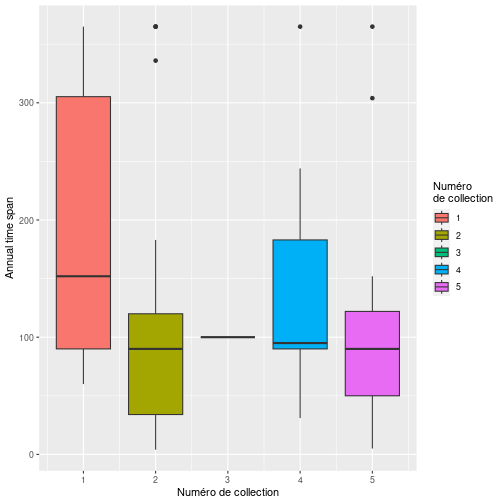
\includegraphics{./img/85d1f067903ecf46ea5379990605207eea6dfa23.png}
\caption{plot of chunk Annual\_timespan\_plot}
\end{figure}

\hypertarget{ruxe9partition-dans-les-clusters-selon-la-taxonomie}{%
\subsubsection{Répartition dans les clusters selon la
taxonomie}\label{ruxe9partition-dans-les-clusters-selon-la-taxonomie}}

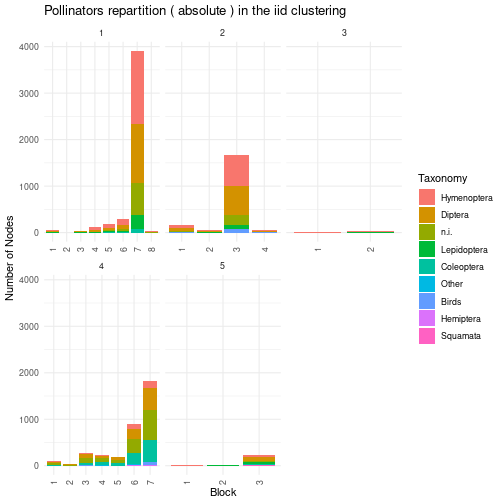
\includegraphics{./img/0bd4d6aa00bf51bbf8e966b7664bea52ace7bede.png}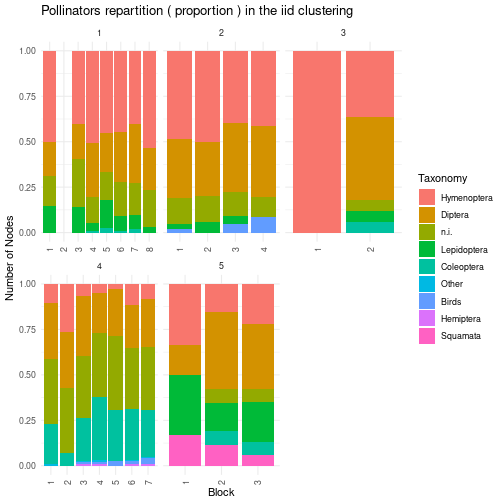
\includegraphics{./img/ba57007c0b13d1fdaa06e6b689f6aaa356359870.png}

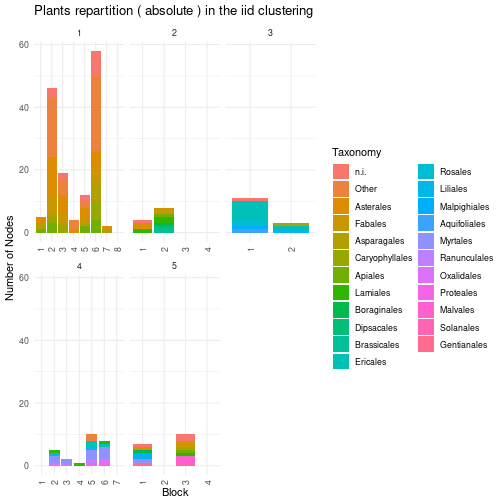
\includegraphics{./img/482a3d80d6f3afab8ca8818d634d42ce2fc8e6d0.png}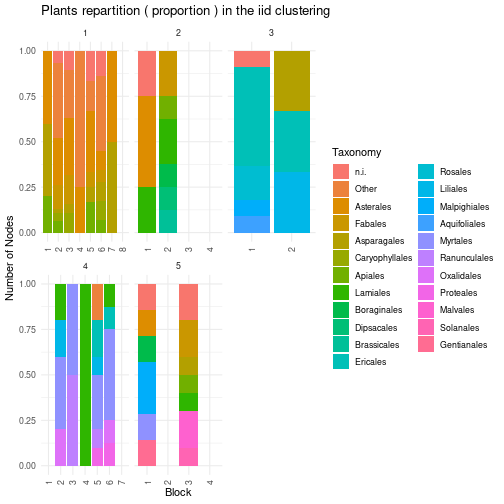
\includegraphics{./img/05f987b57c85b14df8f5e89bf0e380ecc9721edc.png}

\hypertarget{tables}{%
\paragraph{Tables}\label{tables}}

\begin{verbatim}
## # A tibble: 9 × 25
##   Taxon       Collection_1_Bloc_1 Collection_1_Bloc_2 Collection_1_Bloc_3
##   <fct>                     <dbl>               <dbl>               <dbl>
## 1 Hymenoptera                  24                   0                  17
## 2 Diptera                       9                   0                   8
## 3 n.i.                          8                   0                  11
## 4 Lepidoptera                   7                   0                   6
## 5 Coleoptera                    0                   0                   0
## 6 Other                         0                   0                   0
## 7 Birds                        NA                  NA                  NA
## 8 Hemiptera                    NA                  NA                  NA
## 9 Squamata                     NA                  NA                  NA
## # ℹ 21 more variables: Collection_1_Bloc_4 <dbl>, Collection_1_Bloc_5 <dbl>,
## #   Collection_1_Bloc_6 <dbl>, Collection_1_Bloc_7 <dbl>,
## #   Collection_1_Bloc_8 <dbl>, Collection_2_Bloc_1 <dbl>,
## #   Collection_2_Bloc_2 <dbl>, Collection_2_Bloc_3 <dbl>,
## #   Collection_2_Bloc_4 <dbl>, Collection_3_Bloc_1 <dbl>,
## #   Collection_3_Bloc_2 <dbl>, Collection_4_Bloc_1 <dbl>,
## #   Collection_4_Bloc_2 <dbl>, Collection_4_Bloc_3 <dbl>, …
\end{verbatim}

\hypertarget{clustering-with-model-pi}{%
\subsection{Clustering with model pi}\label{clustering-with-model-pi}}

Avec le modèle \emph{pi} nous obtenons les 2 collections et les
structures suivantes:

\subsubsection{Pour la collection 1 }

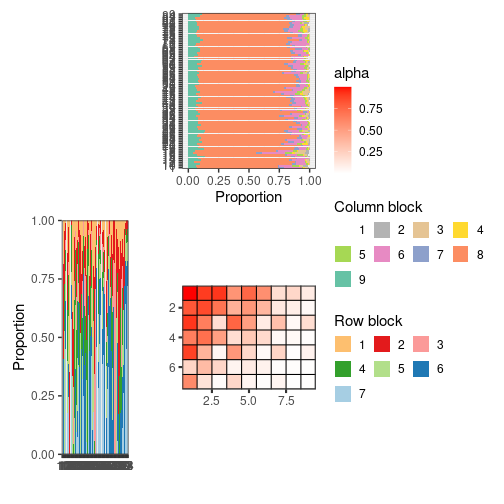
\includegraphics{./img/c8d33c523cb7b1b863840ffe9f838cc1a4dafff2.png}\newline \tiny

\begin{tabular}{l}
\toprule
Networks\\
\midrule
arroyo1982\_1+arroyo1982\_2+arroyo3\\
eberling1999\\
inouye1988\\
kato1990\\
ramirez1992\\
\addlinespace
petanidou1991\\
ramirez1989\\
smith-ramirez2005\\
Junker2013\\
Kaiser\_control+Kaiser\_restored\\
\addlinespace
bartomeus2008\\
Olito-Fox2014\\
Benadi2013\_1(950m)+Benadi2013\_2(1170m)+Benadi2013\_6(2020m)\\
Benadi2013\_3(1340m)\\
Benadi2013\_4(1700m)+Benadi2013\_5(1800m)\\
\addlinespace
Kaiser-Bunbury2017\_Bernica+Kaiser-Bunbury2017\_Casse-dent+Kaiser-Bunbury2017\_Copolia+Kaiser-Bunbury2017\_La-Reserve+Kaiser-Bunbury2017\_Rosebelle+Kaiser-Bunbury2017\_Salazie+Kaiser-Bunbury2017\_Tea-Plantation+Kaiser-Bunbury2017\_Trois-Freres\\
Fang2012\\
Shay2016\\
Struck1994\\
Kato2000\\
\addlinespace
Aizen2008\_Cerro Otto\_U+Aizen2008\_Cerro Otto\_D\\
Aizen2008\_Llao-llao\_U+Aizen2008\_Llao-llao\_D\\
Aizen2008\_Puerto Blest\_U+Aizen2008\_Puerto Blest\_D\\
Albrecht2010\_49yr+Albrecht2010\_63yr+Albrecht2010\_84yr+Albrecht2010\_109yr+Albrecht2010\_130yr\\
Baldock2011\_TB+Baldock2011\_JN\\
\addlinespace
Chamberlain\_cr1+Chamberlain\_cr2+Chamberlain\_fs1+Chamberlain\_fs2+Chamberlain\_go1+Chamberlain\_go2+Chamberlain\_mm1+Chamberlain\_mm2+Chamberlain\_mz1+Chamberlain\_mz2+Chamberlain\_sm1+Chamberlain\_sm2\\
Chamberlain\_HLU+Chamberlain\_HLG+Chamberlain\_OKU+Chamberlain\_OKG+Chamberlain\_WLU+Chamberlain\_WLG+Chamberlain\_SOU+Chamberlain\_SOG\\
Chamberlain\_Site1+Chamberlain\_Site2+Chamberlain\_Site3+Chamberlain\_Site4+Chamberlain\_Site5+Chamberlain\_Site6\\
Dattilo2016\\
Devoto2005\_PP+Devoto2005\_AP\\
\addlinespace
Devoto2005\_VT\\
Devoto2005\_LL+Devoto2005\_CT\\
Dupont2009\_IsenBjerg+Dupont2009\_Other\\
Freitas2006\\
Gibson2006\_TA1\\
\addlinespace
Gibson2006\_TA2\\
Jedrzejewska2013\_Ochata+Jedrzejewska2013\_Kabaty\\
LaraRomero2016\_pe?alara\_EP+LaraRomero2016\_pe?alara\_PA+LaraRomero2016\_nevero\_EP+LaraRomero2016\_nevero\_PA\\
LemusJimenez2003\\
Marrero2013\\
\addlinespace
MonteroCastano2017\_Albufera+MonteroCastano2017\_Llimpa+MonteroCastano2017\_Tirant\\
Kehinde2014\_Joostenberg\_Conv+Kehinde2014\_Joostenberg\_Org+Kehinde2014\_Joostenberg\_Nat+Kehinde2014\_Laibach\_Conv+Kehinde2014\_Laibach\_Org+Kehinde2014\_Laibach\_Nat+Kehinde2014\_Spier\_Conv+Kehinde2014\_Spier\_Nat\\
Pinheiro2008\\
Trojelsgaard2015\_La Gomera\\
Trojelsgaard2015\_Tenerife Teno Bajo+Trojelsgaard2015\_Tenerife Fasnia\\
\addlinespace
Vanbergen2013\_balfarm+Vanbergen2013\_bridgend+Vanbergen2013\_dalhaikie+Vanbergen2013\_netherton+Vanbergen2013\_backhill+Vanbergen2013\_corntulloch+Vanbergen2013\_allancreich\\
Zackenberg\\
Yoshihara2008\\
Watts2016\_Chicon+Watts2016\_Mantanay+Watts2016\_Choquebamba+Watts2016\_Huaran+Watts2016\_Piscacucho+Watts2016\_Poques+Watts2016\_Pumamarca+Watts2016\_Tiaparo+Watts2016\_Yanacocha\\
Kato1993\\
\addlinespace
KatoMiura1996\\
Kakutani1990\\
Inoue1990\\
Fragoso\_RA2+Fragoso\_RA3+Fragoso\_RD1+Fragoso\_RD3\\
PopicThesis\\
\addlinespace
Pfeiffer\_CNE+Pfeiffer\_CNM+Pfeiffer\_CNT+Pfeiffer\_CPB+Pfeiffer\_CPM+Pfeiffer\_CPR+Pfeiffer\_CPS+Pfeiffer\_M2+Pfeiffer\_RP1+Pfeiffer\_RP2+Pfeiffer\_LM+Pfeiffer\_LO+Pfeiffer\_BD+Pfeiffer\_BH+Pfeiffer\_BS\\
Carstensen\_Gigante+Carstensen\_Paulino+Carstensen\_Tinkerbell+Carstensen\_Midway+Carstensen\_Cedro+Carstensen\_Elefante+Carstensen\_Soizig\\
Orford\_B1+Orford\_B2+Orford\_B3+Orford\_B4+Orford\_B5+Orford\_B10\\
Orford\_B6+Orford\_B7+Orford\_B8+Orford\_B9\\
Blumel2016\\
\addlinespace
Welti\_ID+Welti\_K1B+Welti\_K4A+Welti\_4B+Welti\_20B+Welti\_20C+Welti\_N1A+Welti\_N1B+Welti\_N4A+Welti\_N4B+Welti\_N20A+Welti\_N20B\\
Souza\_cerrado\\
Souza\_chaco\\
Souza\_pantanal\\
Souza\_vereda\\
\addlinespace
Grass2013\_1+Grass2013\_2+Grass2013\_3+Grass2013\_4+Grass2013\_5+Grass2013\_6+Grass2013\_7+Grass2013\_8+Grass2013\_9+Grass2013\_10+Grass2013\_11+Grass2013\_12+Grass2013\_13+Grass2013\_14+Grass2013\_15+Grass2013\_16+Grass2013\_17\\
Bennett2018\\
Adedoja2018b\_baseZone+Adedoja2018b\_MidZone+Adedoja2018b\_HighZone+Adedoja2018b\_PeakZone\\
Adedoja2019\\
CordenizPicanco2018\_NatVeg\\
\addlinespace
Benadi2018\\
Hackett2019\_NZ\_salt\_marsh+Hackett2019\_NZ\_sand\_dune+Hackett2019\_NZ\_scrub\_coprosma\\
Oleques2019\\
Jolls2019\\
Traveset2013\_Fernandina\\
\addlinespace
Traveset2013\_Santiago\\
Traveset2013\_SantaCruz\\
Traveset2013\_SanCristobal\\
Simanonok2014\\
Son2019\_a1+Son2019\_a2+Son2019\_a3+Son2019\_a4+Son2019\_a5+Son2019\_a6+Son2019\_a7+Son2019\_a8+Son2019\_F1+Son2019\_F2+Son2019\_F3+Son2019\_F4+Son2019\_F5+Son2019\_F6+Son2019\_F7+Son2019\_F8\\
\addlinespace
Baldock2019\_Bristol\\
Baldock2019\_Edinburgh\\
Baldock2019\_Leeds\\
Baldock2019\_Reading\\
\bottomrule
\end{tabular}

\normalsize\newline\[\begin{pmatrix} 1 &0.9 &0.92 &0.55 &0.75 &0.57 &0.17 \\0.1 &0.21 &0.81 &0.86 &0.7 &0.4 &0.54 \\0.38 &0.12 &0.03 &0.09 &0.92 &0.65 &0.17 \\0.76 &0.5 &0.1 &0.33 &0.17 &0.04 &0.65 \\0.71 &0.5 &0.18 &0.28 &0.19 &0.04 &0.01 \\0.03 &0.89 &0.4 &0.05 &0.53 &0.2 &0.03 \\0.22 &0.07 &0.01 &0.22 &0.35 &0.21 &0.06 \\0.11 &0.07 &0.01 &0.01 &0.01 &0.6 &0.15 \\0.02 &0.21 &0.06 &0.01 &0.06 &0.01 &0 \\ \end{pmatrix}\]

\subsubsection{Pour la collection 2 }

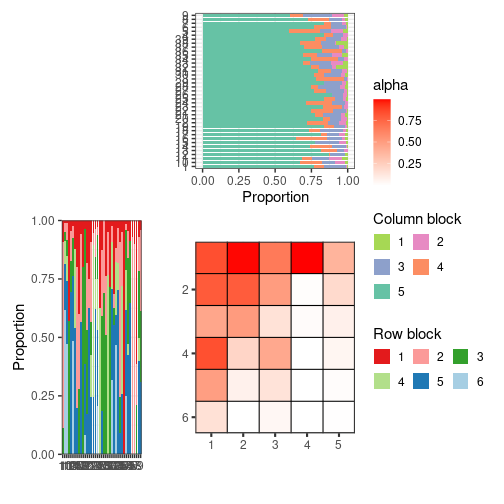
\includegraphics{./img/66882e0b770527a45b5ba01441cbb86ed71491bd.png}\newline \tiny

\begin{tabular}{l}
\toprule
Networks\\
\midrule
dupont2003\\
herrera1988\\
medan2002ld\\
medan2002rb\\
olensen2002aig\\
\addlinespace
olensen2002flo\\
small1976\\
vazquez2002\\
Burkle2013\\
Weiner2011\\
\addlinespace
Gilarranz2014\_amarante+Gilarranz2014\_barrosa+Gilarranz2014\_cincocerros+Gilarranz2014\_difuntito+Gilarranz2014\_difuntos+Gilarranz2014\_elmorro+Gilarranz2014\_labrava+Gilarranz2014\_lachata+Gilarranz2014\_lapaja+Gilarranz2014\_piedraalta+Gilarranz2014\_vigilancia+Gilarranz2014\_volcan\\
Aizen2008\_Challhuaco\_U+Aizen2008\_Challhuaco\_D\\
Devoto2005\_LQ\\
Devoto2005\_LT+Devoto2005\_LH\\
Gibson2006\_GA1\\
\addlinespace
Gibson2006\_GA2\\
Gibson2006\_SG\\
Lundgren2005\\
Trojelsgaard2015\_El Hierro\\
Trojelsgaard2015\_Gran Canaria\\
\addlinespace
Trojelsgaard2015\_Fuerteventura\\
Trojelsgaard2015\_Western Sahara\\
Fragoso\_RA1+Fragoso\_RD2\\
Pornon2017\\
Kantsa2018\\
\addlinespace
Robinson2018\\
CordenizPicanco2018\_NatFor\\
CordenizPicanco2018\_ExoFor\\
CordenizPicanco2018\_SemiPast\\
CordenizPicanco2018\_IntPast\\
\addlinespace
Hackett2019\_UK\_sand\_dune+Hackett2019\_UK\_grassland+Hackett2019\_UK\_heathland+Hackett2019\_UK\_woodland+Hackett2019\_UK\_salt\_marsh+Hackett2019\_UK\_scrub\\
Biella2019\\
Nel2017\\
Villalobos2019\\
LaraRomero2019\_blanca+LaraRomero2019\_rajada+LaraRomero2019\_refugio+LaraRomero2019\_torre\\
\addlinespace
Traveset2013\_Pinta\\
Ferrero2013\\
Neli2014\\
Sritongchuay2019\_near+Sritongchuay2019\_far\\
\bottomrule
\end{tabular}

\normalsize\newline\[\begin{pmatrix} 0.84 &0.99 &0.66 &0.99 &0.38 &0.79 \\0.79 &0.5 &0.01 &0.19 &0.46 &0.51 \\0.15 &0.02 &0.08 &0.83 &0.22 &0.44 \\0 &0.05 &0.49 &0.07 &0.15 &0 \\0.01 &0.16 &0 &0.04 &0 &0 \\ \end{pmatrix}\]

Et voici donc les valeurs numériques pour les \(\alpha\) (paramètres de
connectivité).

Pour la collection 1 :
\[\begin{pmatrix} 1 &0.9 &0.92 &0.55 &0.75 &0.57 &0.17 \\0.1 &0.21 &0.81 &0.86 &0.7 &0.4 &0.54 \\0.38 &0.12 &0.03 &0.09 &0.92 &0.65 &0.17 \\0.76 &0.5 &0.1 &0.33 &0.17 &0.04 &0.65 \\0.71 &0.5 &0.18 &0.28 &0.19 &0.04 &0.01 \\0.03 &0.89 &0.4 &0.05 &0.53 &0.2 &0.03 \\0.22 &0.07 &0.01 &0.22 &0.35 &0.21 &0.06 \\0.11 &0.07 &0.01 &0.01 &0.01 &0.6 &0.15 \\0.02 &0.21 &0.06 &0.01 &0.06 &0.01 &0 \\ \end{pmatrix}\]
Pour la collection 2 :
\[\begin{pmatrix} 0.84 &0.99 &0.66 &0.99 &0.38 &0.79 \\0.79 &0.5 &0.01 &0.19 &0.46 &0.51 \\0.15 &0.02 &0.08 &0.83 &0.22 &0.44 \\0 &0.05 &0.49 &0.07 &0.15 &0 \\0.01 &0.16 &0 &0.04 &0 &0 \\ \end{pmatrix}\]

\hypertarget{ruxe9partition-dans-les-clusters-selon-la-taxonomie-1}{%
\subsubsection{Répartition dans les clusters selon la
taxonomie}\label{ruxe9partition-dans-les-clusters-selon-la-taxonomie-1}}

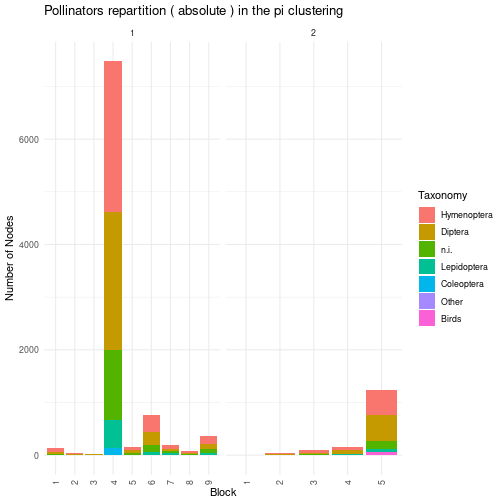
\includegraphics{./img/ff78b3a602b38666524674a6e38d94ee26963376.png}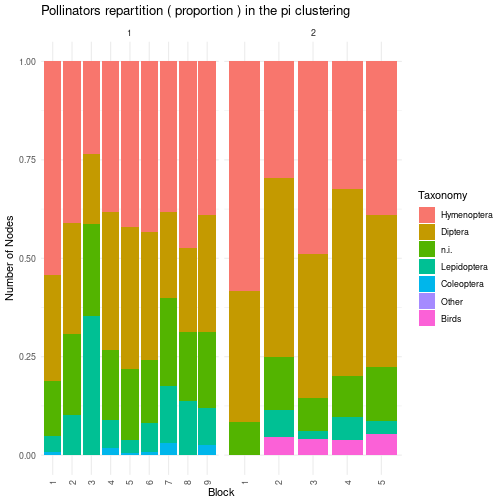
\includegraphics{./img/57ebffb0873b5079093d6f7d474c00142ee5e2ab.png}

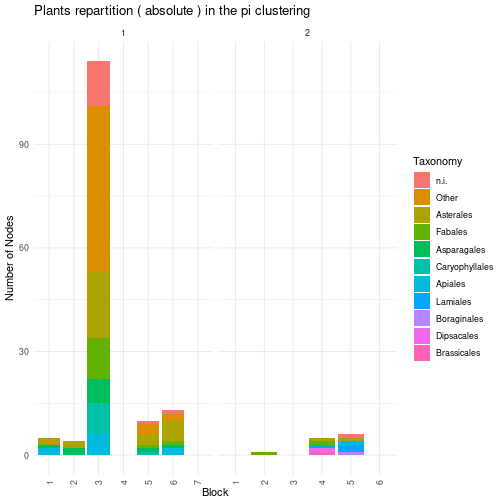
\includegraphics{./img/1616c974be02698dd5c80725494a650ced9db214.png}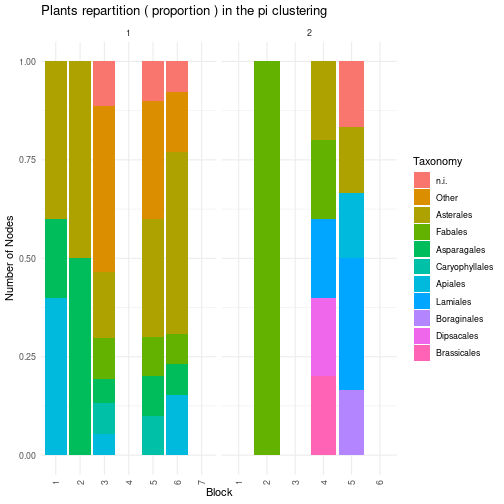
\includegraphics{./img/b7dacdc5d5ad116b7b9b2c16dcd4084230bcf8cf.png}

\hypertarget{clustering-with-model-rho}{%
\subsection{Clustering with model rho}\label{clustering-with-model-rho}}

Avec le modèle \emph{rho} nous obtenons les 1 collections et les
structures suivantes:

\subsubsection{Pour la collection 1 }

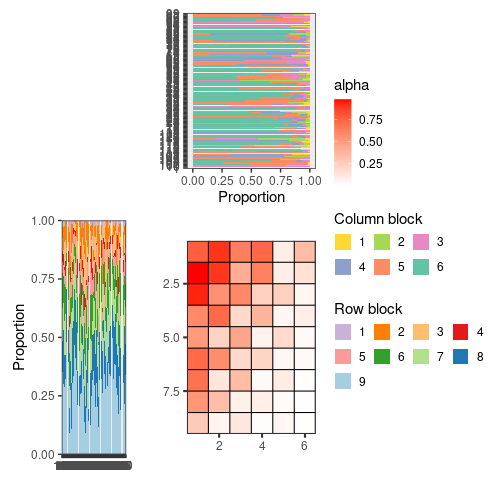
\includegraphics{./img/ddafd83b5651fceb6261e4b7a7637e13859cac33.png}\newline \tiny

\begin{tabular}{l}
\toprule
Networks\\
\midrule
arroyo1982\_1+arroyo1982\_2+arroyo3\\
dupont2003\\
eberling1999\\
herrera1988\\
inouye1988\\
\addlinespace
kato1990\\
medan2002ld\\
medan2002rb\\
olensen2002aig\\
olensen2002flo\\
\addlinespace
ramirez1992\\
small1976\\
vazquez2002\\
petanidou1991\\
ramirez1989\\
\addlinespace
smith-ramirez2005\\
Burkle2013\\
Junker2013\\
Weiner2011\\
Kaiser\_control+Kaiser\_restored\\
\addlinespace
bartomeus2008\\
Olito-Fox2014\\
Gilarranz2014\_amarante+Gilarranz2014\_barrosa+Gilarranz2014\_cincocerros+Gilarranz2014\_difuntito+Gilarranz2014\_difuntos+Gilarranz2014\_elmorro+Gilarranz2014\_labrava+Gilarranz2014\_lachata+Gilarranz2014\_lapaja+Gilarranz2014\_piedraalta+Gilarranz2014\_vigilancia+Gilarranz2014\_volcan\\
Benadi2013\_1(950m)+Benadi2013\_2(1170m)+Benadi2013\_6(2020m)\\
Benadi2013\_3(1340m)\\
\addlinespace
Benadi2013\_4(1700m)+Benadi2013\_5(1800m)\\
Kaiser-Bunbury2017\_Bernica+Kaiser-Bunbury2017\_Casse-dent+Kaiser-Bunbury2017\_Copolia+Kaiser-Bunbury2017\_La-Reserve+Kaiser-Bunbury2017\_Rosebelle+Kaiser-Bunbury2017\_Salazie+Kaiser-Bunbury2017\_Tea-Plantation+Kaiser-Bunbury2017\_Trois-Freres\\
Fang2012\\
Shay2016\\
Struck1994\\
\addlinespace
Kato2000\\
Aizen2008\_Challhuaco\_U+Aizen2008\_Challhuaco\_D\\
Aizen2008\_Cerro Otto\_U+Aizen2008\_Cerro Otto\_D\\
Aizen2008\_Llao-llao\_U+Aizen2008\_Llao-llao\_D\\
Aizen2008\_Puerto Blest\_U+Aizen2008\_Puerto Blest\_D\\
\addlinespace
Albrecht2010\_49yr+Albrecht2010\_63yr+Albrecht2010\_84yr+Albrecht2010\_109yr+Albrecht2010\_130yr\\
Baldock2011\_TB+Baldock2011\_JN\\
Chamberlain\_cr1+Chamberlain\_cr2+Chamberlain\_fs1+Chamberlain\_fs2+Chamberlain\_go1+Chamberlain\_go2+Chamberlain\_mm1+Chamberlain\_mm2+Chamberlain\_mz1+Chamberlain\_mz2+Chamberlain\_sm1+Chamberlain\_sm2\\
Chamberlain\_HLU+Chamberlain\_HLG+Chamberlain\_OKU+Chamberlain\_OKG+Chamberlain\_WLU+Chamberlain\_WLG+Chamberlain\_SOU+Chamberlain\_SOG\\
Chamberlain\_Site1+Chamberlain\_Site2+Chamberlain\_Site3+Chamberlain\_Site4+Chamberlain\_Site5+Chamberlain\_Site6\\
\addlinespace
Dattilo2016\\
Devoto2005\_LQ\\
Devoto2005\_PP+Devoto2005\_AP\\
Devoto2005\_LT+Devoto2005\_LH\\
Devoto2005\_VT\\
\addlinespace
Devoto2005\_LL+Devoto2005\_CT\\
Dupont2009\_IsenBjerg+Dupont2009\_Other\\
Freitas2006\\
Gibson2006\_GA1\\
Gibson2006\_GA2\\
\addlinespace
Gibson2006\_SG\\
Gibson2006\_TA1\\
Gibson2006\_TA2\\
Jedrzejewska2013\_Ochata+Jedrzejewska2013\_Kabaty\\
LaraRomero2016\_pe?alara\_EP+LaraRomero2016\_pe?alara\_PA+LaraRomero2016\_nevero\_EP+LaraRomero2016\_nevero\_PA\\
\addlinespace
LemusJimenez2003\\
Lundgren2005\\
Marrero2013\\
MonteroCastano2017\_Albufera+MonteroCastano2017\_Llimpa+MonteroCastano2017\_Tirant\\
Kehinde2014\_Joostenberg\_Conv+Kehinde2014\_Joostenberg\_Org+Kehinde2014\_Joostenberg\_Nat+Kehinde2014\_Laibach\_Conv+Kehinde2014\_Laibach\_Org+Kehinde2014\_Laibach\_Nat+Kehinde2014\_Spier\_Conv+Kehinde2014\_Spier\_Nat\\
\addlinespace
Pinheiro2008\\
Trojelsgaard2015\_El Hierro\\
Trojelsgaard2015\_La Gomera\\
Trojelsgaard2015\_Gran Canaria\\
Trojelsgaard2015\_Fuerteventura\\
\addlinespace
Trojelsgaard2015\_Tenerife Teno Bajo+Trojelsgaard2015\_Tenerife Fasnia\\
Trojelsgaard2015\_Western Sahara\\
Vanbergen2013\_balfarm+Vanbergen2013\_bridgend+Vanbergen2013\_dalhaikie+Vanbergen2013\_netherton+Vanbergen2013\_backhill+Vanbergen2013\_corntulloch+Vanbergen2013\_allancreich\\
Zackenberg\\
Yoshihara2008\\
\addlinespace
Watts2016\_Chicon+Watts2016\_Mantanay+Watts2016\_Choquebamba+Watts2016\_Huaran+Watts2016\_Piscacucho+Watts2016\_Poques+Watts2016\_Pumamarca+Watts2016\_Tiaparo+Watts2016\_Yanacocha\\
Kato1993\\
KatoMiura1996\\
Kakutani1990\\
Inoue1990\\
\addlinespace
Fragoso\_RA1+Fragoso\_RD2\\
Fragoso\_RA2+Fragoso\_RA3+Fragoso\_RD1+Fragoso\_RD3\\
PopicThesis\\
Pfeiffer\_CNE+Pfeiffer\_CNM+Pfeiffer\_CNT+Pfeiffer\_CPB+Pfeiffer\_CPM+Pfeiffer\_CPR+Pfeiffer\_CPS+Pfeiffer\_M2+Pfeiffer\_RP1+Pfeiffer\_RP2+Pfeiffer\_LM+Pfeiffer\_LO+Pfeiffer\_BD+Pfeiffer\_BH+Pfeiffer\_BS\\
Carstensen\_Gigante+Carstensen\_Paulino+Carstensen\_Tinkerbell+Carstensen\_Midway+Carstensen\_Cedro+Carstensen\_Elefante+Carstensen\_Soizig\\
\addlinespace
Pornon2017\\
Orford\_B1+Orford\_B2+Orford\_B3+Orford\_B4+Orford\_B5+Orford\_B10\\
Orford\_B6+Orford\_B7+Orford\_B8+Orford\_B9\\
Blumel2016\\
Welti\_ID+Welti\_K1B+Welti\_K4A+Welti\_4B+Welti\_20B+Welti\_20C+Welti\_N1A+Welti\_N1B+Welti\_N4A+Welti\_N4B+Welti\_N20A+Welti\_N20B\\
\addlinespace
Kantsa2018\\
Souza\_cerrado\\
Souza\_chaco\\
Souza\_pantanal\\
Souza\_vereda\\
\addlinespace
Grass2013\_1+Grass2013\_2+Grass2013\_3+Grass2013\_4+Grass2013\_5+Grass2013\_6+Grass2013\_7+Grass2013\_8+Grass2013\_9+Grass2013\_10+Grass2013\_11+Grass2013\_12+Grass2013\_13+Grass2013\_14+Grass2013\_15+Grass2013\_16+Grass2013\_17\\
Robinson2018\\
Bennett2018\\
Adedoja2018b\_baseZone+Adedoja2018b\_MidZone+Adedoja2018b\_HighZone+Adedoja2018b\_PeakZone\\
Adedoja2019\\
\addlinespace
CordenizPicanco2018\_NatFor\\
CordenizPicanco2018\_NatVeg\\
CordenizPicanco2018\_ExoFor\\
CordenizPicanco2018\_SemiPast\\
CordenizPicanco2018\_IntPast\\
\addlinespace
Benadi2018\\
Hackett2019\_NZ\_salt\_marsh+Hackett2019\_NZ\_sand\_dune+Hackett2019\_NZ\_scrub\_coprosma\\
Hackett2019\_UK\_sand\_dune+Hackett2019\_UK\_grassland+Hackett2019\_UK\_heathland+Hackett2019\_UK\_woodland+Hackett2019\_UK\_salt\_marsh+Hackett2019\_UK\_scrub\\
Oleques2019\\
Biella2019\\
\addlinespace
Jolls2019\\
Nel2017\\
Villalobos2019\\
LaraRomero2019\_blanca+LaraRomero2019\_rajada+LaraRomero2019\_refugio+LaraRomero2019\_torre\\
Traveset2013\_Fernandina\\
\addlinespace
Traveset2013\_Pinta\\
Traveset2013\_Santiago\\
Traveset2013\_SantaCruz\\
Traveset2013\_SanCristobal\\
Ferrero2013\\
\addlinespace
Simanonok2014\\
Son2019\_a1+Son2019\_a2+Son2019\_a3+Son2019\_a4+Son2019\_a5+Son2019\_a6+Son2019\_a7+Son2019\_a8+Son2019\_F1+Son2019\_F2+Son2019\_F3+Son2019\_F4+Son2019\_F5+Son2019\_F6+Son2019\_F7+Son2019\_F8\\
Neli2014\\
Sritongchuay2019\_near+Sritongchuay2019\_far\\
Baldock2019\_Bristol\\
\addlinespace
Baldock2019\_Edinburgh\\
Baldock2019\_Leeds\\
Baldock2019\_Reading\\
\bottomrule
\end{tabular}

\normalsize\newline\[\begin{pmatrix} 0.77 &0.91 &0.64 &0.73 &0.09 &0.34 &0.98 &0.9 &0.41 \\0.63 &0.09 &0.15 &0.94 &0.56 &0.6 &0.25 &0.24 &0.05 \\0.59 &0.73 &0.19 &0.38 &0.04 &0.09 &0.51 &0.22 &0.46 \\0.07 &0.19 &0.02 &0.73 &0.58 &0.2 &0.22 &0.04 &0.03 \\0.69 &0.13 &0.34 &0.03 &0.1 &0.01 &0.53 &0.33 &0.08 \\0.09 &0.02 &0.01 &0.27 &0.06 &0.12 &0.01 &0.04 &0 \\ \end{pmatrix}\]

Et voici donc les valeurs numériques pour les \(\alpha\) (paramètres de
connectivité).

Pour la collection 1 :
\[\begin{pmatrix} 0.77 &0.91 &0.64 &0.73 &0.09 &0.34 &0.98 &0.9 &0.41 \\0.63 &0.09 &0.15 &0.94 &0.56 &0.6 &0.25 &0.24 &0.05 \\0.59 &0.73 &0.19 &0.38 &0.04 &0.09 &0.51 &0.22 &0.46 \\0.07 &0.19 &0.02 &0.73 &0.58 &0.2 &0.22 &0.04 &0.03 \\0.69 &0.13 &0.34 &0.03 &0.1 &0.01 &0.53 &0.33 &0.08 \\0.09 &0.02 &0.01 &0.27 &0.06 &0.12 &0.01 &0.04 &0 \\ \end{pmatrix}\]

\hypertarget{ruxe9partition-dans-les-clusters-selon-la-taxonomie-2}{%
\subsubsection{Répartition dans les clusters selon la
taxonomie}\label{ruxe9partition-dans-les-clusters-selon-la-taxonomie-2}}

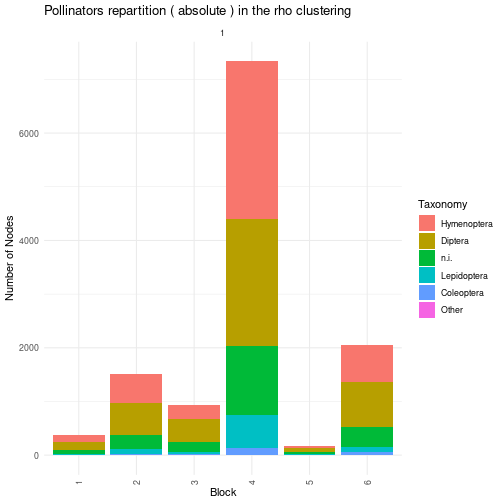
\includegraphics{./img/35ffbce157e0b3bb2a32af4dbc7faa201c946a6b.png}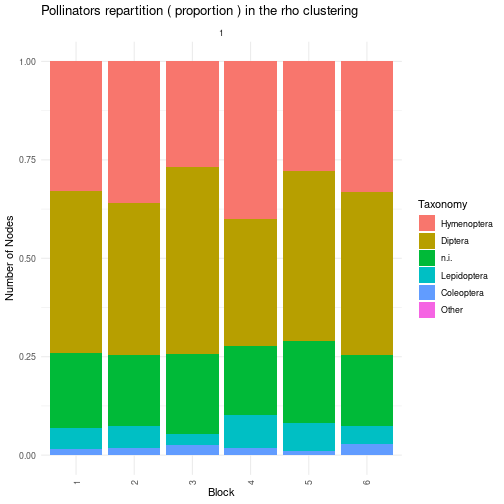
\includegraphics{./img/62d45913b19d56f0ab48a367e53b8ed8fa83c2cc.png}

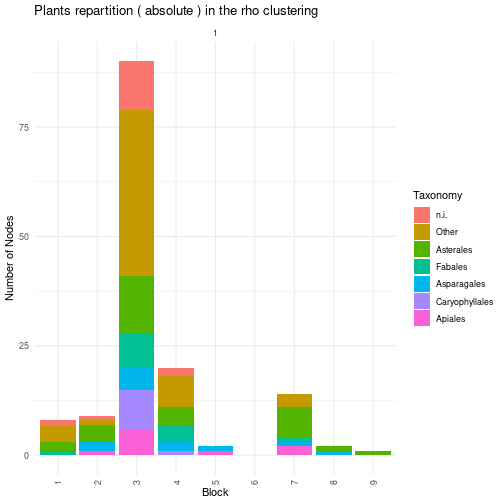
\includegraphics{./img/d1f52d1df28195df25bdfd2bf18f50a176d52c90.png}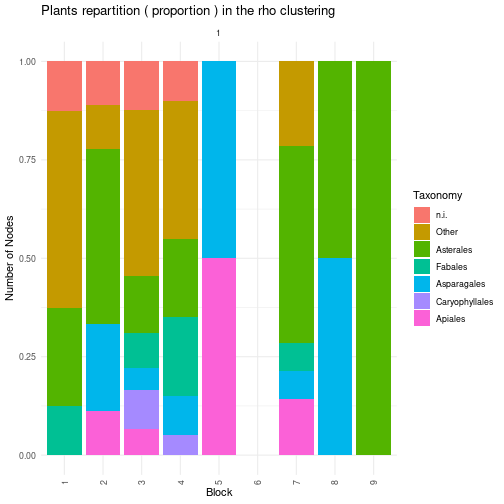
\includegraphics{./img/ce6571ff09f37636eff0631a2269c77055df1403.png}

\hypertarget{clustering-with-model-pirho}{%
\subsection{Clustering with model
pirho}\label{clustering-with-model-pirho}}

Avec le modèle \emph{pirho} nous obtenons les 15 collections et les
structures suivantes:

\subsubsection{Pour la collection 1 }

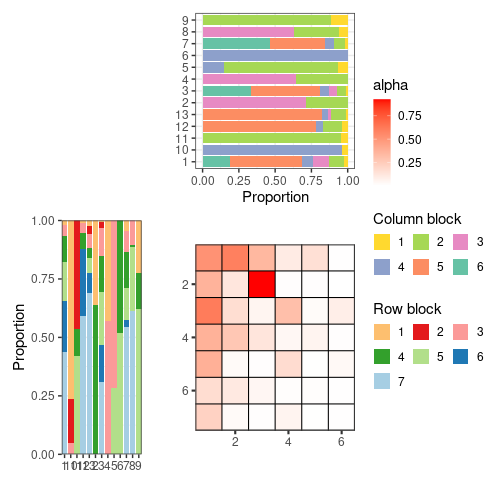
\includegraphics{./img/1b76f16cf61f19fcd2cd382227f1c1dafbdd86b8.png}\newline \tiny

\begin{tabular}{l}
\toprule
Networks\\
\midrule
arroyo1982\_1+arroyo1982\_2+arroyo3\\
dupont2003\\
petanidou1991\\
Aizen2008\_Challhuaco\_U+Aizen2008\_Challhuaco\_D\\
Aizen2008\_Llao-llao\_U+Aizen2008\_Llao-llao\_D\\
\addlinespace
Jedrzejewska2013\_Ochata+Jedrzejewska2013\_Kabaty\\
Pinheiro2008\\
Souza\_pantanal\\
Robinson2018\\
Jolls2019\\
\addlinespace
Traveset2013\_Fernandina\\
Baldock2019\_Leeds\\
Baldock2019\_Reading\\
\bottomrule
\end{tabular}

\normalsize\newline\[\begin{pmatrix} 0.52 &0.6 &0.34 &0.1 &0.15 &0 &0.36 \\0.12 &0.93 &0.01 &0.01 &0 &0.61 &0.16 \\0.05 &0.31 &0.02 &0.08 &0.37 &0.27 &0.12 \\0.04 &0.05 &0.01 &0.38 &0.03 &0.01 &0.17 \\0 &0.03 &0.16 &0.11 &0.04 &0.01 &0.01 \\0.01 &0.22 &0.02 &0.01 &0.05 &0 &0.01 \\ \end{pmatrix}\]

\subsubsection{Pour la collection 2 }

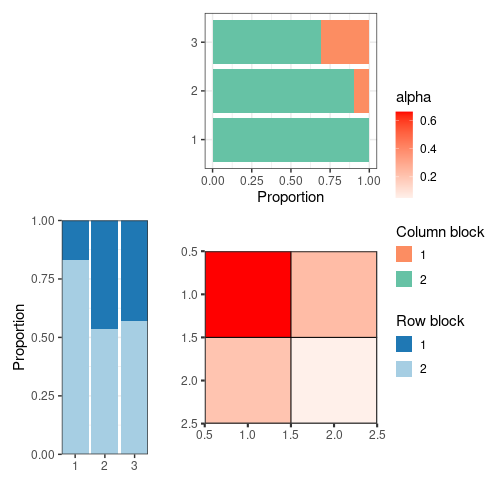
\includegraphics{./img/9a6b30dad9046620bd49013adaef8960862792a2.png}\newline \tiny

\begin{tabular}{l}
\toprule
Networks\\
\midrule
Benadi2013\_3(1340m)\\
Trojelsgaard2015\_La Gomera\\
CordenizPicanco2018\_SemiPast\\
\bottomrule
\end{tabular}

\normalsize\newline\[\begin{pmatrix} 0.66 &0.23 \\0.2 &0.05 \\ \end{pmatrix}\]

\subsubsection{Pour la collection 3 }

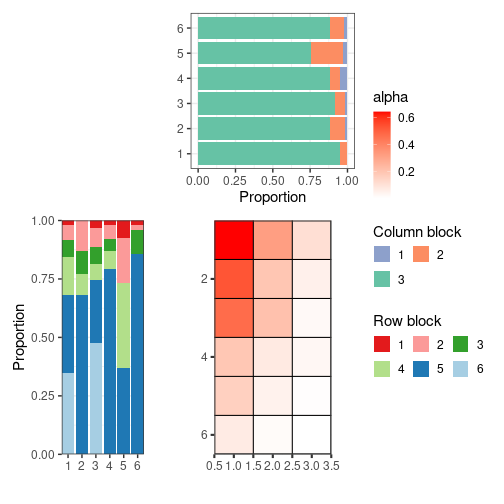
\includegraphics{./img/b8abb8188b0bc33c6f0544fed1eb1ff74aac349a.png}\newline \tiny

\begin{tabular}{l}
\toprule
Networks\\
\midrule
Kato2000\\
Freitas2006\\
Inoue1990\\
Souza\_cerrado\\
Adedoja2019\\
\addlinespace
Baldock2019\_Bristol\\
\bottomrule
\end{tabular}

\normalsize\newline\[\begin{pmatrix} 0.64 &0.32 &0.11 &0.53 &0.19 &0.05 \\0.47 &0.21 &0.02 &0.19 &0.07 &0.03 \\0.16 &0.05 &0.01 &0.07 &0.01 &0 \\ \end{pmatrix}\]

\subsubsection{Pour la collection 4 }

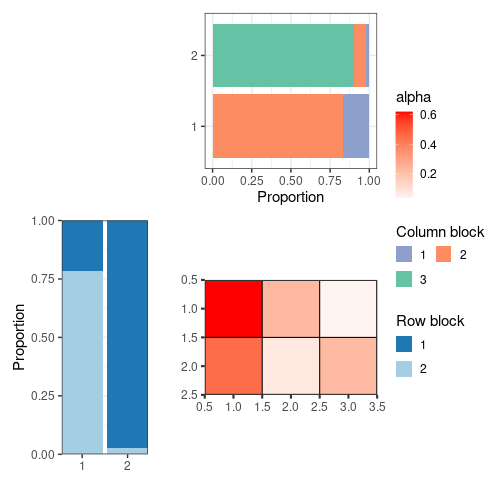
\includegraphics{./img/73d8481e68a1a4993a0eda2edcc5b2a65ac241c2.png}\newline \tiny

\begin{tabular}{l}
\toprule
Networks\\
\midrule
Aizen2008\_Puerto Blest\_U+Aizen2008\_Puerto Blest\_D\\
LemusJimenez2003\\
\bottomrule
\end{tabular}

\normalsize\newline\[\begin{pmatrix} 0.45 &0.07 \\0.22 &0.62 \\0.23 &0.04 \\ \end{pmatrix}\]

\subsubsection{Pour la collection 5 }

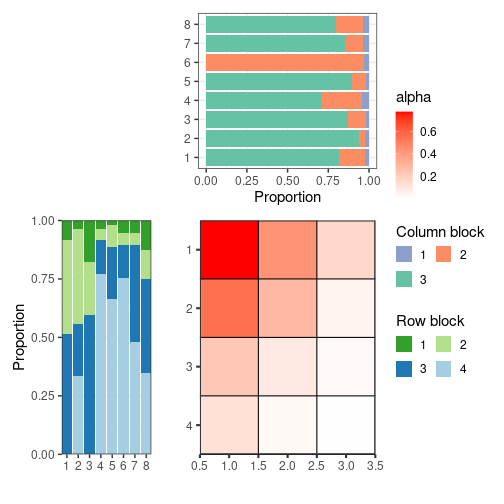
\includegraphics{./img/f5433f933dadae33c549c51d26316f90eb2bbdcd.png}\newline \tiny

\begin{tabular}{l}
\toprule
Networks\\
\midrule
inouye1988\\
Junker2013\\
Kehinde2014\_Joostenberg\_Conv+Kehinde2014\_Joostenberg\_Org+Kehinde2014\_Joostenberg\_Nat+Kehinde2014\_Laibach\_Conv+Kehinde2014\_Laibach\_Org+Kehinde2014\_Laibach\_Nat+Kehinde2014\_Spier\_Conv+Kehinde2014\_Spier\_Nat\\
Watts2016\_Chicon+Watts2016\_Mantanay+Watts2016\_Choquebamba+Watts2016\_Huaran+Watts2016\_Piscacucho+Watts2016\_Poques+Watts2016\_Pumamarca+Watts2016\_Tiaparo+Watts2016\_Yanacocha\\
Kakutani1990\\
\addlinespace
Fragoso\_RA1+Fragoso\_RD2\\
Souza\_chaco\\
Oleques2019\\
\bottomrule
\end{tabular}

\normalsize\newline\[\begin{pmatrix} 0.78 &0.43 &0.16 &0.56 \\0.29 &0.04 &0.22 &0.08 \\0.02 &0.12 &0.03 &0 \\ \end{pmatrix}\]

\subsubsection{Pour la collection 6 }

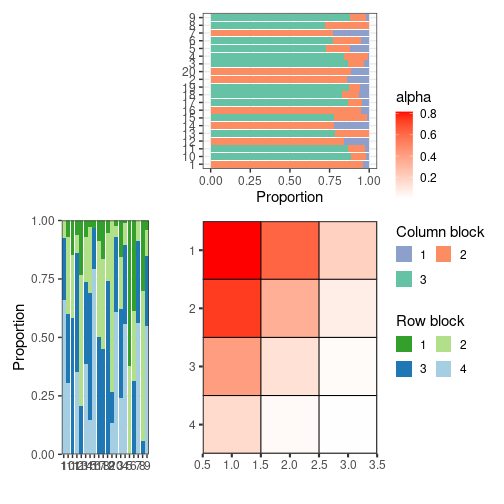
\includegraphics{./img/9b8b977552f9856c8f2569fd0a1796c7df59125e.png}\newline \tiny

\begin{tabular}{l}
\toprule
Networks\\
\midrule
medan2002ld\\
small1976\\
smith-ramirez2005\\
Benadi2013\_1(950m)+Benadi2013\_2(1170m)+Benadi2013\_6(2020m)\\
Shay2016\\
\addlinespace
Aizen2008\_Cerro Otto\_U+Aizen2008\_Cerro Otto\_D\\
Lundgren2005\\
Zackenberg\\
Carstensen\_Gigante+Carstensen\_Paulino+Carstensen\_Tinkerbell+Carstensen\_Midway+Carstensen\_Cedro+Carstensen\_Elefante+Carstensen\_Soizig\\
Welti\_ID+Welti\_K1B+Welti\_K4A+Welti\_4B+Welti\_20B+Welti\_20C+Welti\_N1A+Welti\_N1B+Welti\_N4A+Welti\_N4B+Welti\_N20A+Welti\_N20B\\
\addlinespace
Bennett2018\\
CordenizPicanco2018\_NatFor\\
CordenizPicanco2018\_ExoFor\\
CordenizPicanco2018\_IntPast\\
Benadi2018\\
\addlinespace
Villalobos2019\\
Traveset2013\_Santiago\\
Traveset2013\_SantaCruz\\
Son2019\_a1+Son2019\_a2+Son2019\_a3+Son2019\_a4+Son2019\_a5+Son2019\_a6+Son2019\_a7+Son2019\_a8+Son2019\_F1+Son2019\_F2+Son2019\_F3+Son2019\_F4+Son2019\_F5+Son2019\_F6+Son2019\_F7+Son2019\_F8\\
Sritongchuay2019\_near+Sritongchuay2019\_far\\
\bottomrule
\end{tabular}

\normalsize\newline\[\begin{pmatrix} 0.82 &0.63 &0.2 &0.74 \\0.34 &0.07 &0.41 &0.13 \\0.02 &0.16 &0.03 &0 \\ \end{pmatrix}\]

\subsubsection{Pour la collection 7 }

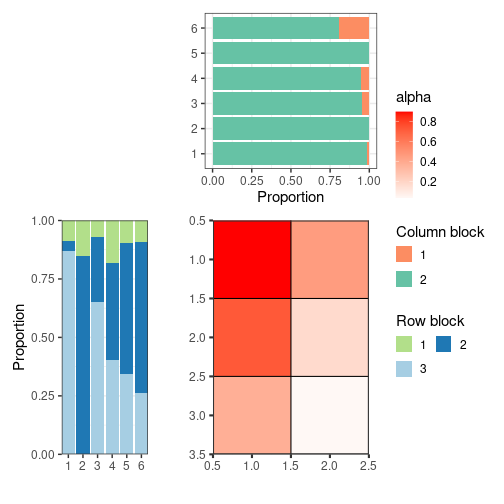
\includegraphics{./img/2bc2aa5f9522a80d234598c960d2b148c78a0bf0.png}\newline \tiny

\begin{tabular}{l}
\toprule
Networks\\
\midrule
medan2002rb\\
olensen2002flo\\
vazquez2002\\
Trojelsgaard2015\_Gran Canaria\\
Trojelsgaard2015\_Western Sahara\\
\addlinespace
LaraRomero2019\_blanca+LaraRomero2019\_rajada+LaraRomero2019\_refugio+LaraRomero2019\_torre\\
\bottomrule
\end{tabular}

\normalsize\newline\[\begin{pmatrix} 0.9 &0.46 &0.72 \\0.17 &0.37 &0.03 \\ \end{pmatrix}\]

\subsubsection{Pour la collection 8 }

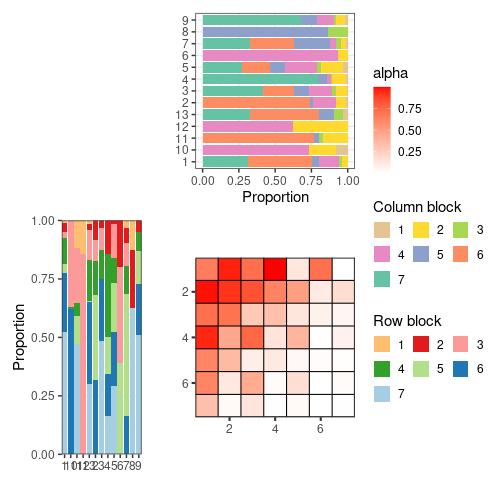
\includegraphics{./img/2435c20b207156887cade4b89b0572d42c93ab82.png}\newline \tiny

\begin{tabular}{l}
\toprule
Networks\\
\midrule
Weiner2011\\
Kaiser\_control+Kaiser\_restored\\
Gilarranz2014\_amarante+Gilarranz2014\_barrosa+Gilarranz2014\_cincocerros+Gilarranz2014\_difuntito+Gilarranz2014\_difuntos+Gilarranz2014\_elmorro+Gilarranz2014\_labrava+Gilarranz2014\_lachata+Gilarranz2014\_lapaja+Gilarranz2014\_piedraalta+Gilarranz2014\_vigilancia+Gilarranz2014\_volcan\\
Kaiser-Bunbury2017\_Bernica+Kaiser-Bunbury2017\_Casse-dent+Kaiser-Bunbury2017\_Copolia+Kaiser-Bunbury2017\_La-Reserve+Kaiser-Bunbury2017\_Rosebelle+Kaiser-Bunbury2017\_Salazie+Kaiser-Bunbury2017\_Tea-Plantation+Kaiser-Bunbury2017\_Trois-Freres\\
Fang2012\\
\addlinespace
Gibson2006\_SG\\
Gibson2006\_TA1\\
Trojelsgaard2015\_Fuerteventura\\
Pfeiffer\_CNE+Pfeiffer\_CNM+Pfeiffer\_CNT+Pfeiffer\_CPB+Pfeiffer\_CPM+Pfeiffer\_CPR+Pfeiffer\_CPS+Pfeiffer\_M2+Pfeiffer\_RP1+Pfeiffer\_RP2+Pfeiffer\_LM+Pfeiffer\_LO+Pfeiffer\_BD+Pfeiffer\_BH+Pfeiffer\_BS\\
Biella2019\\
\addlinespace
Nel2017\\
Ferrero2013\\
Neli2014\\
\bottomrule
\end{tabular}

\normalsize\newline\[\begin{pmatrix} 0.66 &0.97 &0.72 &1 &0.13 &0.71 &0 \\0.99 &0.93 &0.84 &0.64 &0.5 &0.11 &0.17 \\0.71 &0.7 &0.28 &0.32 &0.13 &0.07 &0.05 \\0.96 &0.46 &0.75 &0.14 &0.39 &0.01 &0.07 \\0.62 &0.36 &0.09 &0.11 &0.04 &0.02 &0.01 \\0.62 &0.12 &0.43 &0.02 &0.17 &0 &0.02 \\0.33 &0.03 &0.14 &0 &0.03 &0 &0 \\ \end{pmatrix}\]

\subsubsection{Pour la collection 9 }

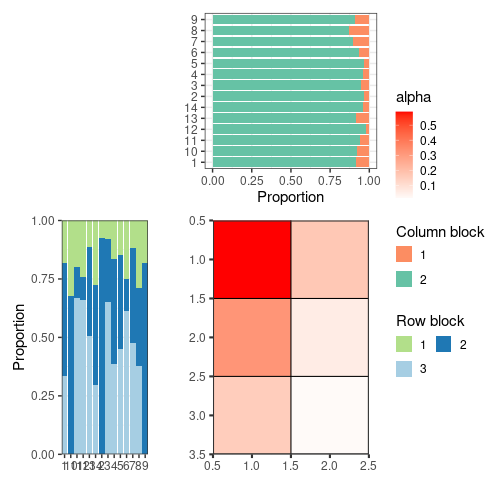
\includegraphics{./img/01cf8becd8b4fa7e13437d68ce7a48e6365fc5d8.png}\newline \tiny

\begin{tabular}{l}
\toprule
Networks\\
\midrule
eberling1999\\
ramirez1992\\
Struck1994\\
Albrecht2010\_49yr+Albrecht2010\_63yr+Albrecht2010\_84yr+Albrecht2010\_109yr+Albrecht2010\_130yr\\
Devoto2005\_PP+Devoto2005\_AP\\
\addlinespace
Devoto2005\_VT\\
Gibson2006\_TA2\\
MonteroCastano2017\_Albufera+MonteroCastano2017\_Llimpa+MonteroCastano2017\_Tirant\\
Yoshihara2008\\
PopicThesis\\
\addlinespace
Orford\_B1+Orford\_B2+Orford\_B3+Orford\_B4+Orford\_B5+Orford\_B10\\
Souza\_vereda\\
Adedoja2018b\_baseZone+Adedoja2018b\_MidZone+Adedoja2018b\_HighZone+Adedoja2018b\_PeakZone\\
Hackett2019\_NZ\_salt\_marsh+Hackett2019\_NZ\_sand\_dune+Hackett2019\_NZ\_scrub\_coprosma\\
\bottomrule
\end{tabular}

\normalsize\newline\[\begin{pmatrix} 0.59 &0.17 &0.32 \\0.06 &0.15 &0.02 \\ \end{pmatrix}\]

\subsubsection{Pour la collection 10 }

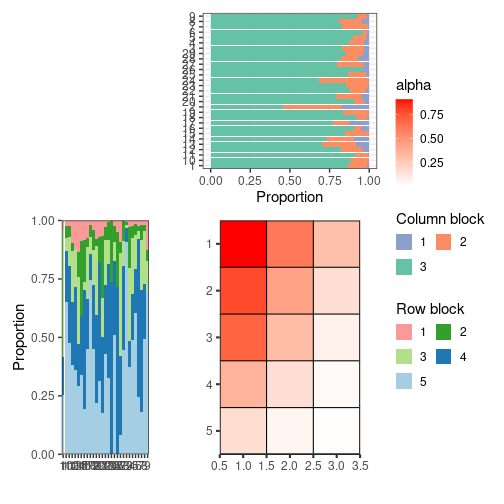
\includegraphics{./img/f191d6381b05b4f2f4139e717eebf1075211d7ea.png}\newline \tiny

\begin{tabular}{l}
\toprule
Networks\\
\midrule
herrera1988\\
Burkle2013\\
bartomeus2008\\
Olito-Fox2014\\
Benadi2013\_4(1700m)+Benadi2013\_5(1800m)\\
\addlinespace
Baldock2011\_TB+Baldock2011\_JN\\
Chamberlain\_HLU+Chamberlain\_HLG+Chamberlain\_OKU+Chamberlain\_OKG+Chamberlain\_WLU+Chamberlain\_WLG+Chamberlain\_SOU+Chamberlain\_SOG\\
Chamberlain\_Site1+Chamberlain\_Site2+Chamberlain\_Site3+Chamberlain\_Site4+Chamberlain\_Site5+Chamberlain\_Site6\\
Devoto2005\_LQ\\
Devoto2005\_LT+Devoto2005\_LH\\
\addlinespace
Devoto2005\_LL+Devoto2005\_CT\\
Dupont2009\_IsenBjerg+Dupont2009\_Other\\
Gibson2006\_GA1\\
LaraRomero2016\_pe?alara\_EP+LaraRomero2016\_pe?alara\_PA+LaraRomero2016\_nevero\_EP+LaraRomero2016\_nevero\_PA\\
Marrero2013\\
\addlinespace
Trojelsgaard2015\_Tenerife Teno Bajo+Trojelsgaard2015\_Tenerife Fasnia\\
Vanbergen2013\_balfarm+Vanbergen2013\_bridgend+Vanbergen2013\_dalhaikie+Vanbergen2013\_netherton+Vanbergen2013\_backhill+Vanbergen2013\_corntulloch+Vanbergen2013\_allancreich\\
Fragoso\_RA2+Fragoso\_RA3+Fragoso\_RD1+Fragoso\_RD3\\
Pornon2017\\
Orford\_B6+Orford\_B7+Orford\_B8+Orford\_B9\\
\addlinespace
Blumel2016\\
Kantsa2018\\
Grass2013\_1+Grass2013\_2+Grass2013\_3+Grass2013\_4+Grass2013\_5+Grass2013\_6+Grass2013\_7+Grass2013\_8+Grass2013\_9+Grass2013\_10+Grass2013\_11+Grass2013\_12+Grass2013\_13+Grass2013\_14+Grass2013\_15+Grass2013\_16+Grass2013\_17\\
CordenizPicanco2018\_NatVeg\\
Hackett2019\_UK\_sand\_dune+Hackett2019\_UK\_grassland+Hackett2019\_UK\_heathland+Hackett2019\_UK\_woodland+Hackett2019\_UK\_salt\_marsh+Hackett2019\_UK\_scrub\\
\addlinespace
Traveset2013\_Pinta\\
Traveset2013\_SanCristobal\\
Simanonok2014\\
Baldock2019\_Edinburgh\\
\bottomrule
\end{tabular}

\normalsize\newline\[\begin{pmatrix} 0.91 &0.62 &0.3 &0.79 &0.44 \\0.15 &0.7 &0.32 &0.07 &0.36 \\0.15 &0.03 &0.16 &0.05 &0.01 \\ \end{pmatrix}\]

\subsubsection{Pour la collection 11 }

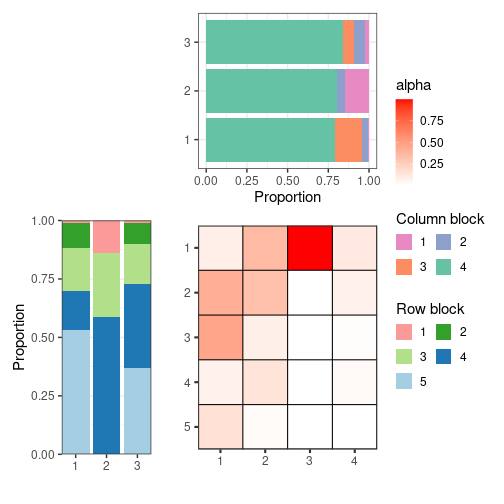
\includegraphics{./img/b890876aef1a920f5fdc0fb91d549ad59455c587.png}\newline \tiny

\begin{tabular}{l}
\toprule
Networks\\
\midrule
kato1990\\
ramirez1989\\
Kato1993\\
\bottomrule
\end{tabular}

\normalsize\newline\[\begin{pmatrix} 0.09 &0.36 &1 &0.12 &0.41 \\0.33 &0 &0.07 &0.46 &0.09 \\0 &0.01 &0.07 &0.14 &0 \\0.03 &0.16 &0.02 &0 &0 \\ \end{pmatrix}\]

\subsubsection{Pour la collection 12 }

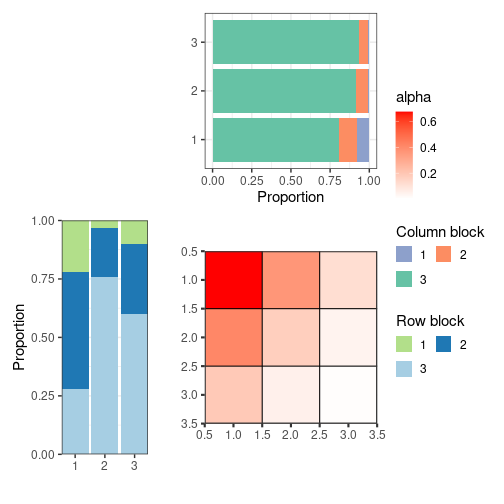
\includegraphics{./img/63fe35c05911cc6ad732c2424d821e1ff6017bcf.png}\newline \tiny

\begin{tabular}{l}
\toprule
Networks\\
\midrule
Chamberlain\_cr1+Chamberlain\_cr2+Chamberlain\_fs1+Chamberlain\_fs2+Chamberlain\_go1+Chamberlain\_go2+Chamberlain\_mm1+Chamberlain\_mm2+Chamberlain\_mz1+Chamberlain\_mz2+Chamberlain\_sm1+Chamberlain\_sm2\\
Dattilo2016\\
KatoMiura1996\\
\bottomrule
\end{tabular}

\normalsize\newline\[\begin{pmatrix} 0.68 &0.37 &0.12 \\0.41 &0.17 &0.04 \\0.19 &0.05 &0.01 \\ \end{pmatrix}\]

\subsubsection{Pour la collection 13 }

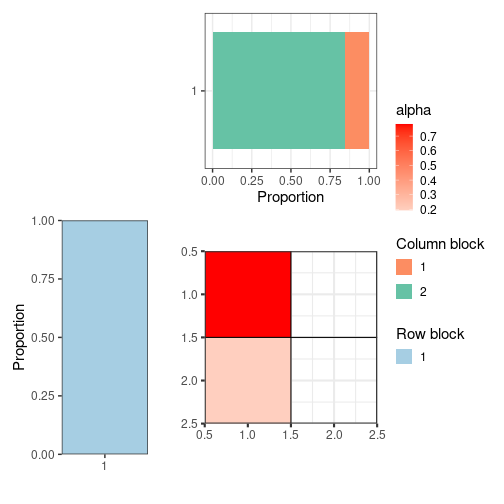
\includegraphics{./img/3c15b096f5435091aae32ed4477d5df277c2af82.png}\newline \tiny

\begin{tabular}{l}
\toprule
Networks\\
\midrule
olensen2002aig\\
\bottomrule
\end{tabular}

\normalsize\newline\[\begin{pmatrix} 0.78 \\0.19 \\ \end{pmatrix}\]

\subsubsection{Pour la collection 14 }

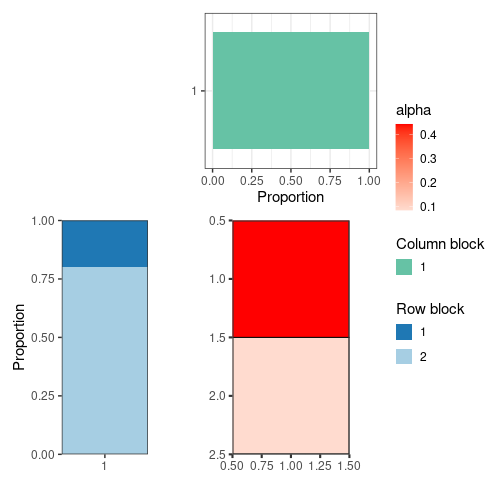
\includegraphics{./img/888bd40e8c6409a43aae4aa9744e362b2ea7da34.png}\newline \tiny

\begin{tabular}{l}
\toprule
Networks\\
\midrule
Trojelsgaard2015\_El Hierro\\
\bottomrule
\end{tabular}

\normalsize\newline\[\begin{pmatrix} 0.44 &0.08 \\ \end{pmatrix}\]

\subsubsection{Pour la collection 15 }

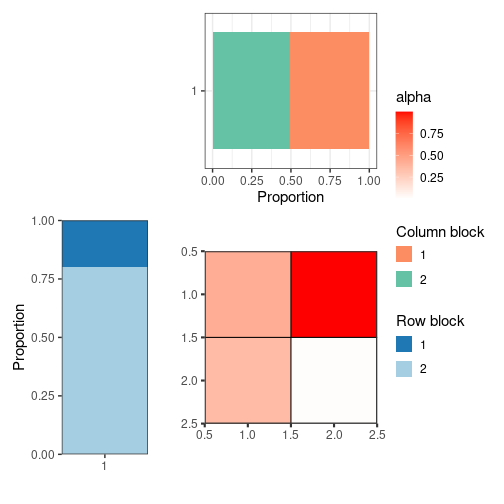
\includegraphics{./img/be03e1e125628e702f825f4e55f2a3d50d226045.png}\newline \tiny

\begin{tabular}{l}
\toprule
Networks\\
\midrule
Gibson2006\_GA2\\
\bottomrule
\end{tabular}

\normalsize\newline\[\begin{pmatrix} 0.42 &1 \\0.35 &0.01 \\ \end{pmatrix}\]

Et voici donc les valeurs numériques pour les \(\alpha\) (paramètres de
connectivité).

Pour la collection 1 :
\[\begin{pmatrix} 0.52 &0.6 &0.34 &0.1 &0.15 &0 &0.36 \\0.12 &0.93 &0.01 &0.01 &0 &0.61 &0.16 \\0.05 &0.31 &0.02 &0.08 &0.37 &0.27 &0.12 \\0.04 &0.05 &0.01 &0.38 &0.03 &0.01 &0.17 \\0 &0.03 &0.16 &0.11 &0.04 &0.01 &0.01 \\0.01 &0.22 &0.02 &0.01 &0.05 &0 &0.01 \\ \end{pmatrix}\]
Pour la collection 2 :
\[\begin{pmatrix} 0.66 &0.23 \\0.2 &0.05 \\ \end{pmatrix}\] Pour la
collection 3 :
\[\begin{pmatrix} 0.64 &0.32 &0.11 &0.53 &0.19 &0.05 \\0.47 &0.21 &0.02 &0.19 &0.07 &0.03 \\0.16 &0.05 &0.01 &0.07 &0.01 &0 \\ \end{pmatrix}\]
Pour la collection 4 :
\[\begin{pmatrix} 0.45 &0.07 \\0.22 &0.62 \\0.23 &0.04 \\ \end{pmatrix}\]
Pour la collection 5 :
\[\begin{pmatrix} 0.78 &0.43 &0.16 &0.56 \\0.29 &0.04 &0.22 &0.08 \\0.02 &0.12 &0.03 &0 \\ \end{pmatrix}\]
Pour la collection 6 :
\[\begin{pmatrix} 0.82 &0.63 &0.2 &0.74 \\0.34 &0.07 &0.41 &0.13 \\0.02 &0.16 &0.03 &0 \\ \end{pmatrix}\]
Pour la collection 7 :
\[\begin{pmatrix} 0.9 &0.46 &0.72 \\0.17 &0.37 &0.03 \\ \end{pmatrix}\]
Pour la collection 8 :
\[\begin{pmatrix} 0.66 &0.97 &0.72 &1 &0.13 &0.71 &0 \\0.99 &0.93 &0.84 &0.64 &0.5 &0.11 &0.17 \\0.71 &0.7 &0.28 &0.32 &0.13 &0.07 &0.05 \\0.96 &0.46 &0.75 &0.14 &0.39 &0.01 &0.07 \\0.62 &0.36 &0.09 &0.11 &0.04 &0.02 &0.01 \\0.62 &0.12 &0.43 &0.02 &0.17 &0 &0.02 \\0.33 &0.03 &0.14 &0 &0.03 &0 &0 \\ \end{pmatrix}\]
Pour la collection 9 :
\[\begin{pmatrix} 0.59 &0.17 &0.32 \\0.06 &0.15 &0.02 \\ \end{pmatrix}\]
Pour la collection 10 :
\[\begin{pmatrix} 0.91 &0.62 &0.3 &0.79 &0.44 \\0.15 &0.7 &0.32 &0.07 &0.36 \\0.15 &0.03 &0.16 &0.05 &0.01 \\ \end{pmatrix}\]
Pour la collection 11 :
\[\begin{pmatrix} 0.09 &0.36 &1 &0.12 &0.41 \\0.33 &0 &0.07 &0.46 &0.09 \\0 &0.01 &0.07 &0.14 &0 \\0.03 &0.16 &0.02 &0 &0 \\ \end{pmatrix}\]
Pour la collection 12 :
\[\begin{pmatrix} 0.68 &0.37 &0.12 \\0.41 &0.17 &0.04 \\0.19 &0.05 &0.01 \\ \end{pmatrix}\]
Pour la collection 13 : \[\begin{pmatrix} 0.78 \\0.19 \\ \end{pmatrix}\]
Pour la collection 14 : \[\begin{pmatrix} 0.44 &0.08 \\ \end{pmatrix}\]
Pour la collection 15 :
\[\begin{pmatrix} 0.42 &1 \\0.35 &0.01 \\ \end{pmatrix}\]

\hypertarget{ruxe9partition-dans-les-clusters-selon-la-taxonomie-3}{%
\subsubsection{Répartition dans les clusters selon la
taxonomie}\label{ruxe9partition-dans-les-clusters-selon-la-taxonomie-3}}

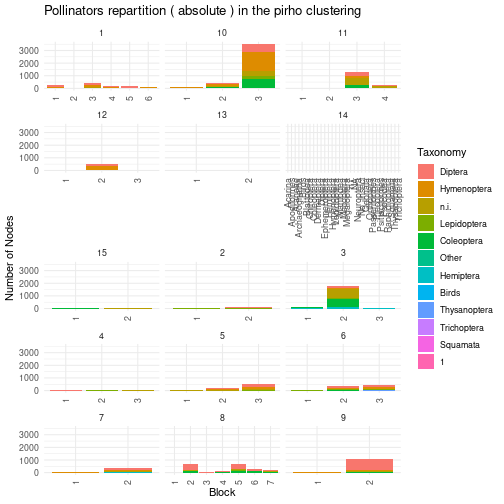
\includegraphics{./img/337973465a11f78731e92a7e62b1f4c2164ab43e.png}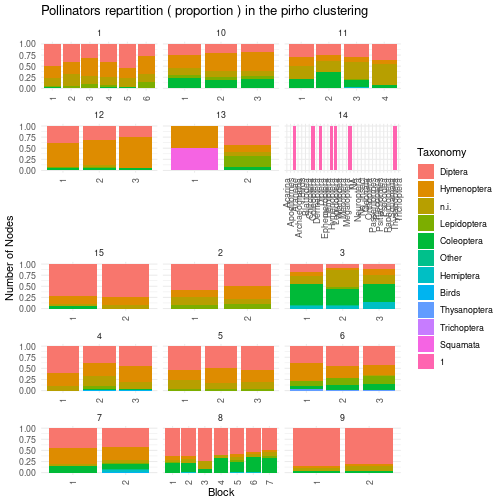
\includegraphics{./img/09bed9592345eff7f0e23841c310114fc4b5773d.png}

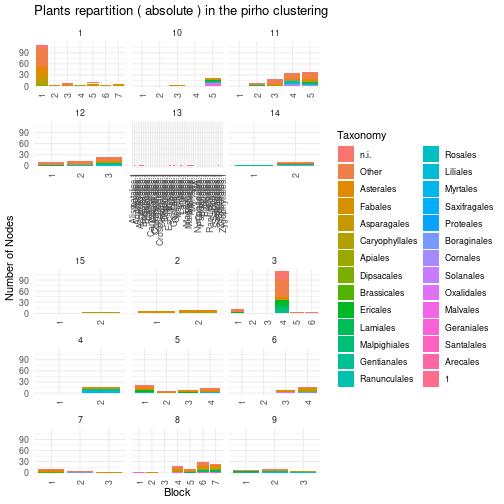
\includegraphics{./img/9e913a77139e5e0a619c6c0e9beef79f87c6bb61.png}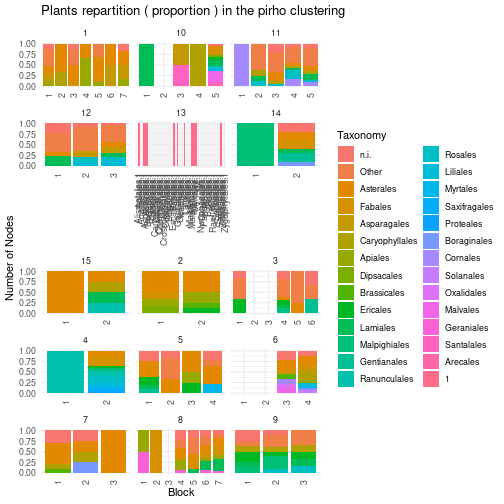
\includegraphics{./img/c3c10578cbfaf01a313454190bda1efad0227b03.png}

\subsection{Completing raw data using CoOPLBM \parencite{anakokDisentanglingStructureEcological2022}}

% Options for packages loaded elsewhere
\PassOptionsToPackage{unicode}{hyperref}
\PassOptionsToPackage{hyphens}{url}
%
\documentclass[
]{article}
\usepackage{lmodern}
\usepackage{amssymb,amsmath}
\usepackage{ifxetex,ifluatex}
\ifnum 0\ifxetex 1\fi\ifluatex 1\fi=0 % if pdftex
  \usepackage[T1]{fontenc}
  \usepackage[utf8]{inputenc}
  \usepackage{textcomp} % provide euro and other symbols
\else % if luatex or xetex
  \usepackage{unicode-math}
  \defaultfontfeatures{Scale=MatchLowercase}
  \defaultfontfeatures[\rmfamily]{Ligatures=TeX,Scale=1}
\fi
% Use upquote if available, for straight quotes in verbatim environments
\IfFileExists{upquote.sty}{\usepackage{upquote}}{}
\IfFileExists{microtype.sty}{% use microtype if available
  \usepackage[]{microtype}
  \UseMicrotypeSet[protrusion]{basicmath} % disable protrusion for tt fonts
}{}
\makeatletter
\@ifundefined{KOMAClassName}{% if non-KOMA class
  \IfFileExists{parskip.sty}{%
    \usepackage{parskip}
  }{% else
    \setlength{\parindent}{0pt}
    \setlength{\parskip}{6pt plus 2pt minus 1pt}}
}{% if KOMA class
  \KOMAoptions{parskip=half}}
\makeatother
\usepackage{xcolor}
\IfFileExists{xurl.sty}{\usepackage{xurl}}{} % add URL line breaks if available
\IfFileExists{bookmark.sty}{\usepackage{bookmark}}{\usepackage{hyperref}}
\hypersetup{
  pdftitle={Netclustering analysis with the CoOPLBM completion},
  hidelinks,
  pdfcreator={LaTeX via pandoc}}
\urlstyle{same} % disable monospaced font for URLs
\usepackage[margin=1in]{geometry}
\usepackage{graphicx}
\makeatletter
\def\maxwidth{\ifdim\Gin@nat@width>\linewidth\linewidth\else\Gin@nat@width\fi}
\def\maxheight{\ifdim\Gin@nat@height>\textheight\textheight\else\Gin@nat@height\fi}
\makeatother
% Scale images if necessary, so that they will not overflow the page
% margins by default, and it is still possible to overwrite the defaults
% using explicit options in \includegraphics[width, height, ...]{}
\setkeys{Gin}{width=\maxwidth,height=\maxheight,keepaspectratio}
% Set default figure placement to htbp
\makeatletter
\def\fps@figure{htbp}
\makeatother
\setlength{\emergencystretch}{3em} % prevent overfull lines
\providecommand{\tightlist}{%
  \setlength{\itemsep}{0pt}\setlength{\parskip}{0pt}}
\setcounter{secnumdepth}{-\maxdimen} % remove section numbering
\newlength{\cslhangindent}
\setlength{\cslhangindent}{1.5em}
\newenvironment{cslreferences}%
  {\setlength{\parindent}{0pt}%
  \everypar{\setlength{\hangindent}{\cslhangindent}}\ignorespaces}%
  {\par}

\title{Netclustering analysis with the CoOPLBM completion}
\author{}
\date{\vspace{-2.5em}}

\begin{document}
\maketitle

\hypertarget{context-of-this-analysis}{%
\section{Context of this analysis}\label{context-of-this-analysis}}

After performing a netclustering on the raw data, we will see if the
detect structure resulting in the clustering comes from the sampling
effort. To test this we will use the CoOPLBM model by Anakok et al.
(2022) to complete the data.

The CoOPLBM model assumes that the observed incidence matrix \(R\) is an
element-wise product of an \(M\) matrix following an LBM and an \(N\)
matrix which elements follow Poisson distributions independent on \(M\).

The model gives us the \(\hat{M}\) matrix, which elements are:

\begin{itemize}
\tightlist
\item
  1 if the interaction was observed
\item
  a probability, that there should be an interaction but it wasn't
  observed
\end{itemize}

This \emph{completed matrix} can be used in different manners to be fed
to the colSBM model.

\hypertarget{threshold-based-completions}{%
\section{Threshold based
completions}\label{threshold-based-completions}}

With the thresholds, the infered incidence matrix obtained by CoOPLBM is
used to generate a completed incidence matrix by the following procedure
: \[X_{ij} = \begin{cases}
  1 & \text{if the value is over the threshold} \\
  0 & \text{else} \\
\end{cases}\]

\hypertarget{completed-threshold}{%
\subsection{0.5 completed threshold}\label{completed-threshold}}

Here, the completion threshold is set to \(0.5\).

\hypertarget{ari-of-networks-clustering-0.5-threshold-vs-raw-data}{%
\subsubsection{ARI of networks clustering: 0.5 threshold vs raw
data}\label{ari-of-networks-clustering-0.5-threshold-vs-raw-data}}

\hypertarget{sample-based-completions}{%
\section{Sample based completions}\label{sample-based-completions}}

The \(M\) matrix is used to sample a new \(X\) matrix which elements are
the realisation of Bernoulli distributions of probability \(M_{i,j}\).
\[\mathbb{P}(X_{i,j} = 1) = M_{i,j} \]

\hypertarget{references}{%
\section*{References}\label{references}}
\addcontentsline{toc}{section}{References}

\hypertarget{refs}{}
\begin{cslreferences}
\leavevmode\hypertarget{ref-anakokDisentanglingStructureEcological2022}{}%
Anakok, Emre, Pierre Barbillon, Colin Fontaine, and Elisa Thebault.
2022. ``Disentangling the Structure of Ecological Bipartite Networks
from Observation Processes.'' arXiv.
\url{http://arxiv.org/abs/2211.16364}.
\end{cslreferences}

\end{document}


\printbibliography
\listoffigures
\listoftables
\end{document}